\documentclass[
    draft,
    pdftex,
    a4paper,
    oneside,
    parskip,
    numbers=noenddot,
    listof=totoc,
    bibliography=totoc,
    hyperfootnotes=false
]{scrreprt}
\setuptoc{toc}{totoc}

\newcommand{\thesistitle}{Automatisches Feedback für objektorientierte Programmierübungen}
\newcommand{\thesistype}{M A S T E R A R B E I T}
\newcommand{\thesistypedesc}{im Fachbereich Elektrotechnik/Informatik \\
    der Universität Kassel}
\newcommand{\thesisauthorname}{Adrian Kunz,\ B.Sc.}
\newcommand{\thesisauthorhomestreet}{***REMOVED***}
\newcommand{\thesisauthorhometown}{***REMOVED***}
\newcommand{\thesisauthormatrikelnumber}{35013235}
\newcommand{\thesisauthoremail}{***REMOVED***}
\newcommand{\thesisdepartment}{Fachgebiet Software Engineering}
\newcommand{\thesisfirstreviewer}{Prof.\ Dr.\ Albert Zündorf}
\newcommand{\thesissecondreviewer}{Prof.\ Dr.\ Claude Draude}
\newcommand{\thesissupervisor}{Sebastian Copei,\ M.Sc.}
\newcommand{\thesisdate}{31.\ März 2022}

% geometry
\usepackage[bindingoffset=1cm, left=2.5cm, right=2.5cm, top=2.5cm, bottom=2.5cm]{geometry}

% Headline
\usepackage{fancyhdr}
\pagestyle{fancy}
\renewcommand{\chaptermark}[1]{\markboth{\thechapter\ #1}{}}
\lhead{\leftmark} \rhead{\thepage}
\cfoot{}
\fancypagestyle{plain}{}

\RedeclareSectionCommand[beforeskip=1.5cm,afterskip=1cm]{chapter}

% Select input encodung, usually utf8 is the best choice, on windows, \usepackage[latin1]{inputenc} maybe required
\usepackage[utf8]{inputenc}
\usepackage[T1]{fontenc}

% Colors
\usepackage{color}
\usepackage{colortbl}

% Tables
\usepackage{tabularx}
\usepackage{multirow}

% Drawing graphs etc.
\usepackage{pgf}
\usepackage{tikz}
\usetikzlibrary{arrows,automata}

% Footnotes
\usepackage{footmisc}

% math
\usepackage{amsmath}
\usepackage{siunitx}

% lists
\usepackage{paralist}

% Figures
\usepackage{graphicx, wrapfig}

% Hyperlinks
\usepackage[hyphens]{url}
\usepackage{hyperref}
\hypersetup{colorlinks, citecolor=black, linkcolor=black, urlcolor=black}

% Minted
\usepackage[chapter]{minted}
%\usemintedstyle{xcode}
\setminted{frame=single,tabsize=2,linenos}

\newmintinline[code]{text}{breaklines}
\newmintinline[mdcode]{md}{breaklines}
\newmintinline[jcode]{java}{breaklines}

\newminted[codeblock]{text}{autogobble,frame=none,linenos=false,breaklines}
\newminted[mdcodeblock]{md}{autogobble,frame=none,linenos=false,breaklines}
\newminted[jcodeblock]{java}{autogobble,frame=none,linenos=false}

\newcommand{\codelisting}[4]{%
    \begin{listing}[htp]
        \inputminted{#1}{#2/#3}
        \caption{#4}
        \label{lst:#3}
    \end{listing}%
}

% list of abbreviations
\usepackage[printonlyused]{acronym}

% Set line pitch
\usepackage{setspace}
\onehalfspacing              % anderthalbzeilig (oder auch \doublespace)

% Todos
\newcommand{\todo}[1]{\textcolor{red}{TODO: #1}}
\newcommand{\todom}[1]{\marginpar{\parbox{1.5cm}{\textcolor{red}{TODO:\\ #1}}}}

%fancyBox
%\usepackage{fancybox}

% Layout corrections (Schusterjungen)
\clubpenalty = 10000
% Layout corrections (Hurenkinder)
\widowpenalty = 10000
\displaywidowpenalty = 10000

% Figures
\usepackage{caption}
\usepackage[hypcap=true,labelformat=simple]{subcaption}
\renewcommand{\thesubfigure}{(\alph{subfigure})}

% Tables
\usepackage{booktabs}

% Frequently used column types
\newcolumntype{C}[1]{>{\centering\arraybackslash}p{#1}} % centering column type with fixed width
\newcolumntype{R}[1]{>{\raggedleft\arraybackslash}p{#1}} % right aligned column type with fixed width
\newcolumntype{L}[1]{>{\raggedright\arraybackslash}p{#1}} % left aligned column type with fixed width

% Shortcuts for referencing floats:
\newcommand{\fig}[1]{\figurename~\ref{#1}} %shortcut for a figure reference
\newcommand{\tab}[1]{Table~\ref{#1}} %shortcut for a table reference
\newcommand{\eq}[1]{(\ref{#1})} %shortcut for an equation reference
\newcommand{\lst}[1]{Listing~\ref{#1}} %shortcut for a listing reference
\newcommand{\sect}[1]{Section~\ref{#1}} %shortcut for a Section reference


\usepackage[ngerman]{babel}
\usepackage{csquotes}
\usepackage{xcolor}
\MakeOuterQuote{"}
\defaulthyphenchar=127

\begin{document}

    \pagenumbering{roman}

    \begin{titlepage}
	%select font without serifs
	\sffamily

	% Logo
	\begin{tabularx}{\textwidth}{@{}l@{}>{\raggedleft\arraybackslash}X@{}r@{}}
		\multirow{2}{*}{
\includegraphics[width=6.8cm]{images/Logo_UniKassel}} &
		\raisebox{-1mm}{\small{Fachbereich Elektrotechnik/Informatik}} \\
		&\raisebox{-1mm}{\small{\thesisdepartment}} &
	\end{tabularx}

	\vspace{2.5cm}

	\begin{center}
		% Title and subtitle
		\huge{\thesistitle}

		\vspace{3cm}

		\renewcommand{\baselinestretch}{1.3}
		\Large{\thesistype}

		\large
		\thesistypedesc
	\end{center}

	\vspace{1.5cm}
	\renewcommand{\baselinestretch}{1}
	\begin{table}[htpb]
		\centering
		\begin{tabular}{ll}
			\\
			Eingereicht von: & \thesisauthorname \\
			Anschrift: & \thesisauthorhomestreet \\
			& \thesisauthorhometown \\
			\\
			Matrikelnummer: & \thesisauthormatrikelnumber \\
			E-Mail: & \thesisauthoremail \\
			\\
			Vorgelegt im: & \thesisdepartment \\
			\\
			Erstprüfer: & \thesisfirstreviewer \\
			Zweitprüferin: & \thesissecondreviewer \\
			\\
			Betreuer: & \thesissupervisor \\
			\\
			Eingereicht am: & \thesisdate \\
		\end{tabular}
	\end{table}

	% font with serifs
	\rmfamily
\end{titlepage}

    \chapter*{Zusammenfassung}

% Inhaltsverzeichnis und Kopfzeile
\addcontentsline{toc}{chapter}{Zusammenfassung}
\markboth{Zusammenfassung}{Zusammenfassung}

Die Bewertung von Programmieraufgaben einer großen Anzahl von Studierenden ist in der Lehre der Informatik zeitaufwändig.
Diese Arbeit schlägt einen Ansatz der Textsuche vor, um mehrere Lösungen gleichzeitig zu bewerten.
Sie stellt Werkzeuge vor, die beim gesamten Bewertungsprozess unterstützen sowie sich und andere Lernsysteme integrieren, um die Produktivität zu steigern.
Um die Anwendbarkeit zu messen, wurde eine Veranstaltung über ein Semester mit der Software bewertet.
Obwohl die Textsuche keine vollautomatische Bewertung erlaubt, konnte dennoch der Aufwand der Bewertenden in der vorliegenden Evaluation um bis zu 65\% reduziert werden.


    \tableofcontents

    \chapter*{Abkürzungsverzeichnis}

% Inhaltsverzeichnis und Kopfzeile
\addcontentsline{toc}{chapter}{Abkürzungsverzeichnis}
\markboth{Abkürzungsverzeichnis}{Abkürzungsverzeichnis}

\begin{acronym}[XXXXXX]
    \acro{api}[API]{Application Programming Interface}
    \acro{ast}[AST]{Abstract Syntax Tree}
    \acro{css}[CSS]{Cascading Style Sheet}
    \acro{cst}[CST]{Concrete Syntax Tree}
    \acro{emf}[EMF]{Eclipse Modeling Framework}
    \acro{gui}[GUI]{Graphical User Interface}
    \acro{html}[HTML]{Hypertext Markup Language}
    \acro{http}[HTTP]{Hypertext Transfer Protocol}
    \acro{id}[ID]{Identifier}
    \acro{ide}[IDE]{Integrated Development Environment}
    \acro{ip}[IP]{Internet Protocol}
    \acro{json}[JSON]{JavaScript Object Notation}
    \acro{jvm}[JVM]{Java Virtual Machine}
    \acro{lsp}[LSP]{Language Server Protocol}
    \acro{pm}[PM]{Programmieren und Modellieren}
    \acro{rest}[REST]{Representational State Transfer}
    \acro{qol}[QoL]{Quality of Life}
    \acro{ui}[UI]{User Interface}
    \acro{vsc}[VSCode]{Visual Studio Code}

    \acro{bzw}[bzw.]{beziehungsweise}
    \acro{dh}[d.h.]{das heißt}
    \acro{etc}[etc.]{et cetera}
    \acro{idR}[i.d.R.]{in der Regel}
    \acro{ggf}[ggf.]{gegebenenfalls}
    \acro{oBdA}[o.B.d.A.]{ohne Beschränkung der Allgemeinheit}
    \acro{usw}[usw.]{und so weiter}
    \acro{uU}[u.U.]{unter Umständen}
    \acro{vgl}[vgl.]{vergleiche}
    \acro{zB}[z.B.]{zum Beispiel}
\end{acronym}


    \pagebreak
    \pagenumbering{arabic}

    \chapter{Einleitung}\label{ch:introduction}

Die Bewertung von Programmieraufgaben in einer Lehrveranstaltung mit vielen Teilnehmenden kann sehr aufwendig sein.
Abhängig von der Aufgabenstellung müssen viele Zeilen Quellcode gelesen und verstanden werden, um eine akkurate Einschätzung der Richtigkeit zu machen.
Die Arbeit der Bewertenden ist meist repetitiv und kann zu Flüchtigkeitsfehlern führen, wodurch Studierende möglicherweise nicht auf Fehler hingewiesen werden und einer Lerngelegenheit entgehen.
Dennoch bearbeitet jeder Studierende die gleichen Aufgaben.
Es sollte folglich naheliegen, dass auch ähnliche oder sogar gleiche Lösungen entstehen.
Diese Arbeit beabsichtigt, dieses Phänomen zu untersuchen und durch Automatisierung die Bewertenden zu entlasten.
Sie beschreibt Werkzeuge, die für diesen Anwendungszweck entwickelt wurden und bei der Bewertung gemäß der Ziele des nachfolgenden Abschnitts~\ref{sec:goals} unterstützen sollen.
Um einen breiteren Kontext zu schaffen, werden in Abschnitt~\ref{sec:related-work} verwandte Arbeiten betrachtet.
Die wissenschaftlichen Ziele werden in Abschnitt~\ref{sec:research-questions} anhand von \acp{rq} gesteckt.
Zuletzt gibt Abschnitt~\ref{sec:structure} eine kurze Übersicht über die Struktur dieser Arbeit.

\section{Zielsetzung}\label{sec:goals}

In dieser Arbeit soll Software entwickelt werden, die bei der Bewertung von Programmieraufgaben unterstützt.
Diese soll die Konzepte Hausaufgabe, Teilaufgaben, Abgaben \ac{bzw} Lösungen, Bewertungen von Teilaufgaben trennen, sodass eine Gesamtbewertung ermöglicht wird.
Insbesondere sollen Teilpunkte aufgezeichnet werden.
Die gleichzeitige Bewertung mehrerer Lösungen soll erfolgend, indem Bewertungen von Teilaufgaben anhand von Codeabschnitten automatisch auf andere Lösungen mit ähnlichem Code übertragen werden.

Die Werkzeuge sollen möglichst unaufdringlich sein, bestehende Ablaufe ergänzen und optional benutzbar sein.
Insbesondere umfasst dies, dass Studierende diese Werkzeuge nicht für die Abgabe verwenden müssen und Bewertungen in einem Format eingereicht werden, dass auch ohne die Werkzeuge verfügbar ist.
Beispielsweise soll die Verwendung von GitHub Classroom als Abgabemechanismus und GitHub Issues als Feedbackformat unterstützt werden.
Anders ausgedrückt sollen die Werkzeuge für diese bestehenden Technologien eine Integration bieten.

\section{Verwandte Arbeiten}\label{sec:related-work}

\todo{
    Yang Hu et al, Re-factoring based Program Repair applied to Programming Assignments;
    Osei-Owusu et al, Grading-Based Test Suite Augmentation;
}

\section{Forschungsfragen}\label{sec:research-questions}

\subsection[\acs{rq}1]{\ac{rq}1: Kann die Bewertung von Programmieraufgaben sinnvoll automatisiert werden?}\label{subsec:rq1-useful-automation}

\todo{
    Relativ große Anzahl von Studierenden, ähnliche Lösungen - Automatisierung bietet sich an.
}

\subsection[\acs{rq}2]{\ac{rq}2: Welcher Mehraufwand wird für die automatisierte Bewertung benötigt?}\label{subsec:rq2-additional-effort}

\todo{
    Tests schreiben, Musterlösung, keiner?
}

\subsection[\acs{rq}3]{\ac{rq}3: Welche Effektivität und Effizienz kann von der Automatisierung erwartet werden?}\label{subsec:rq3-effectivity-efficiency}

\todo{
    Abhängig von Semester, Modul und Kursfortschritt.
}

\subsection[\acs{rq}4]{\ac{rq}4: Wie können Aufgaben formuliert oder angepasst werden, um die Effektivität und Effizienz zu steigern?}\label{subsec:rq4-improve-effectivity-efficiency}

\todo{
    Unter Beibehaltung der ursprünglichen Lehrziele, möglichst durch triviale Änderungen der Anforderungen.
}

\section{Aufbau der Arbeit}\label{sec:structure}

\todo{
    Ablauf des Anwendungsfalls und verwendetete Drittanbieter-Technologien in Grundlagen.
    Verwendung und Umsetzung der neuen Werkzeuge in Implementierung.
    Ausprobieren und erfassen von Daten in Evaluation.
    Auswerten der Daten und Beantwortung der Forschungsfragen in Auswertung.
    Fazit.
    Zukunftspläne.
}

    \chapter{Grundlagen}\label{ch:basics}

\section{Übungskonzept}\label{sec:programming-assignments}

\todo{
    Genauer Ablauf des Lebenszyklus einer Hausaufgabe.
    Personas von Studierenden und Bewertern.
}

\subsection{Ablauf}\label{subsec:workflow}

\todo{
    Konzeption, Punkteberechnung, Bearbeitung, Bewertung, Feedback.
}

\subsection{Studierende}\label{subsec:students}

\todo{
    Kreative Lösungsansätze oder Nachprogrammieren der Vorlesung.
}

\subsection{Betreuer}\label{subsec:teaching-assistants}

\todo{
    Viele Bewertungen am Stück oder nach und nach.
    Akribische Fehlersuche oder flüchtiges Betrachten.
}

\section{Technologien}\label{sec:tech}

\subsection{fulib.org}\label{subsec:fulib.org}

\todo{
    Screenshots?
}

fulib.org ist eine Webanwendung, die bereits 2019 im Rahmen von~\cite{explain} konzipiert und durch~\cite{bachelor-thesis} erweitert wurde.
Sie besteht aus einigen Modulen, die nachfolgend kurz beschrieben werden.

\subsubsection{Scenarios}
Das erste Modul der Anwendung ist ein interaktiver Editor für die Szenario-Sprache aus~\cite{explain}.
Diese besteht aus textuellen Beispielszenarien, die einer festen Grammatik folgen.
Ein Compiler übersetzt die Szenarien in Java-Code und generiert dabei Klassen für ein Datenmodell mit~\cite{fulib}.
In~\cite{bachelor-thesis} wurde erstmals eine Erweiterung der Sprache umgesetzt, die gezielt die Bewertung von Aufgaben ermöglichen sollte.
Dafür wurde spezielle Syntax zur Mustererkennung auf Objektstrukturen entwickelt, die besonders für Fälle geeignet war, in der die Benennung von Variablen, Attributen und Assoziationen nicht festgelegt war.
Nachfolgend wird die Szenario-Sprache und der Editor auf fulib.org nicht weiter betrachtet.
Es handelt sich jedoch um wichtige Hintergründe und Erkenntnisse, die in den Abschnitten~\ref{sec:expanding-fulib.org} und~\ref{sec:renaming-and-refactoring} wieder aufgegriffen werden.

\subsubsection{Docs}
Hier kann die Dokumentation für verwandte Werkzeuge aus dem fulib-Toolkit nachgelesen werden.
Diese wird direkt von den jeweiligen GitHub-Repositories bezogen, ist also nicht Teil der Webanwendung selber.
Insbesondere befindet sich hier das Benutzerhandbuch von fulibFeedback.

\subsubsection{Projects}
Dieser Teil der Webanwendung ist eine Prototyp für eine Online-\ac{ide}.
Dort können Projekte erstellt werden, die im Gegensatz zum Szenario-Editor mehrere Dateien umfassen können.
Insbesondere können hier Gradle- und Java-Dateien betrachtet und bearbeitet werden.
Ein Dateibaum zeigt Ordner und darin befindliche Dateien jeglicher Art.
Mit einem Web-Terminal können beliebige Kommandozeilenbefehle ausgeführt werden, darunter auch die zum Bauen und Ausführen verwendeten Gradle-Befehle.
Die Projekte ermöglichen folglich eine eingeschränkte Form der Anwendungsentwicklung in einer Desktop-\ac{ide}.
Nachfolgend werden Projekte nicht weiter eingesetzt, sie bieten sich jedoch für zukünftige Erweiterungen in Abschnitt~\ref{sec:future-projects} an.

\subsubsection{Assignments}
Das ursprünglich in~\cite{bachelor-thesis} entwickelte Assignments-Modul von fulib.org ist nun erneut Zentrum der Implementierung.
In Abschnitt~\ref{sec:expanding-fulib.org} wird vermehrt beleuchtet, welche Änderungen vorgenommen wurden.
Nun soll zunächst beschrieben werden, wie der Stand des Moduls gegen Ende von~\cite{bachelor-thesis} war.
Vor dieser Arbeit waren die Assignments, eine eigene Bezeichnung für Hausaufgabenblätter, nur auf Aufgaben in der Szenario-Sprache fokussiert.
Mit einfachen Formularen konnten Titel, Beschreibung, Abgabefrist und einige Teilaufgaben definiert werden.
Jede Teilaufgabe bestand mindestens aus Kurzbeschriebung und Punktzahl
Optional konnte eine Teilaufgabe mit Verifizierungscode in der Szenario-Sprache, meist mit der Pattern Matching-Syntax aus~\cite{bachelor-thesis}, ausgestattet werden.
Studierende erhielten nach erfolgreicher Erstellung des Assignments einen Einladungslink, unter dem sie eine Lösung hochladen konnten.
Diese bestand aus einem zusammenhängenden Szenario-Text.
Nach dem Absenden wurde für jede Teilaufgabe der Verifizierungscodes zusammen mit der Lösung ausgeführt.
Bei erfolgreicher Ausführung wurden für die Teilaufgabe volle Punktzahl, im Fehlerfall null Punkte vergeben.
Somit konnte eine Gesamtpunktzahl errechnet werden.

\subsection{Visual Studio Code}\label{subsec:visual-studio-code}

\ac{vsc}\footnote{\url{https://code.visualstudio.com/}} ist ein erweiterbarer Code-Editor von Microsoft.
Neben den Grundfunktionen eines Texteditors hat \ac{vsc} Funktionen zur Entwicklerproduktivitäts wie Syntax-Highlighting und Autovervollständigung.
Durch vorinstallierte Erweiterungen kann Versionsverwaltung mit Git verwendet werden.
Verschiedene Spracherweiterungen ermöglichen bessere Autovervollständigung und Semantisches Highlighting abhängig von Typinformationen sowie die Darstellung von Syntax-Fehlern und Warnmeldung im Quellcode.
Darüber hinaus ist die Anwendung beliebig mit Erweiterungen anpassbar, die aus einem von Microsoft bereitgestellten Marketplace bezogen werden können\footnote{\url{https://marketplace.visualstudio.com/VSCode}}.
Die Schnittstellen für Erweiterungen sind ausführlich dokumentiert und Entwickler können mit geringem Aufwand eigene Erweiterungen publizieren.
Für Spracherweiterung wirbt \ac{vsc} besonders mit dem \ac{lsp} (siehe~\ref{subsec:language-server-protocol}).
In Abschnitt~\ref{sec:fulibFeedback} wird dies genutzt, um die fulibFeedback-Erweiterung zu veröffentichen.

\todom{Vielleicht sollte das wo anders hin?}
\ac{vsc} wurde als Grundlage für diese Arbeit aus zwei Gründen gewählt.
Einerseits ist die Entwicklung von Erweiterungen im Vergleich zu der \ac{ide} IntelliJ IDEA deutlich einfacher, da die Logik mit dem \ac{lsp} wiederverwendbar implementiert werden kann.
IntelliJ IDEA bietet dafür keine eigene Unterstützung, stattdessen müssen Plugins von Dritten
\footnote{\url{https://github.com/gtache/intellij-lsp}\label{fn:intellij-lsp}}
\footnote{\url{https://github.com/lsp4intellij/intellij-lsp-plugin}\label{fn:intellij-lsp-plugin}}
\footnote{\url{https://github.com/ballerina-platform/lsp4intellij}\label{fn:lsp4intellij}}
verwendet werden.
Diese werden teilweise nicht weiterentwickelt\footref{fn:intellij-lsp} \footref{fn:intellij-lsp-plugin}, bieten nur eingeschränkte Funktionen des \ac{lsp}\footnote{\todo{Welche?}}, oder sind nicht mit aktuellen Versionen von IntelliJ IDEA kompatibel\footnote{\todo{Welche?}}.
Andererseits war \ac{vsc} ein vorgegebenes Werkzeug in der Veranstaltung "Programmieren und Modellieren" im Wintersemester 2021/22.
Es bot sich an, für die Bewertung die gleiche \ac{ide} zu benutzen wie die Studierenden zur Lösungserstellung.
Dadurch konnten bestimmte umgebungsabhängige Fehler vermieden werden.

\subsection{Language Server Protocol}\label{subsec:language-server-protocol}

Das \ac{lsp} bezeichnet eine von Microsoft entwickelte Spezifikation\footnote{\url{https://microsoft.github.io/language-server-protocol/}}, die ein Client/Server-Modell für Sprachunterstützung von Code-Editoren und ein zugehöriges Protokoll vorschlägt.
Das standardisierte Protokoll sollte einige Probleme lösen, die sowohl Entwicklern von Editoren als auch von Programmiersprachen bekannt waren.
Diese werden nachfolgend kurz erläutert.

\begin{description}
    \item[Quadratischer Entwicklungsaufwand]
    Im Vordergrund stand das Problem des quadratischen Entwicklungsaufwands ohne ein standardisiertes Protokoll.
    Soll eine neue Programmiersprache Verwendung finden, ist es notwendig, Unterstützung in möglichst vielen Editoren zu implementieren.
    Dies ist teilweise durch Plugins möglich, die von den Sprachautoren bereitgestellt werden können, aber mitunter signifikanten Entwicklungsaufwand benötigen.
    Aus Sicht der Autoren hat jeder Editor andere Schnittstellen und Funktionen, die studiert und angebunden werden müssen.
    Dies kann die Adaption von Sprachen bei begrenztem Entwicklungsbudget einschränken.
    Aus Sicht der Editorautoren ergibt sich ein ähnliches Problem.
    Um einen neuen Editor marktfähig zu machen, sollte dieser eine große Anzahl populärer Programmiersprachen unterstützen.
    Diese können jedoch weitgehend unterschiedliche Schnittstellen und Werkzeuge bereitstellen, abhängig davon, ob die Editorunterstützung von den Sprachautoren bei der Konzeption von Compiler und anderen Tools eingearbeitet wurde.
    Unter Umständen ist es notwendig, große Teile der Syntax und Semantik dieser Sprachen neu zu implementieren, um Editorunterstützung zu ermöglichen.
    Insgesamt ergibt dies bei $n$ Editoren und $m$ Sprachen einen Aufwand von $n \cdot m$ notwendigen Integrationen.
    Mit dem \ac{lsp} wird dieses Problem aus Sicht beider Seiten gelöst.
    Sprachautoren können einen Server bereitstellen, der gegen die Schnittstellen des \ac{lsp} entwickelt wird.
    Der Editor kann beliebige Sprachserver über die gleichen Schnittstellen ansprechen.
    Folglich müssen nur $n + m$ Werkzeuge entwickelt werden.\cite{why-lsp}
    \item[Trennung von Technologien]
    Ein weiterer Vorteil des \acp{lsp} ist die Möglichkeit, Server und Client in unterschiedlichen Programmiersprachen und Frameworks zu entwickeln.
    Dies kann sprachseitig die Serverentwicklung vereinfachen, da beispielsweise Teile der Implementierung des Compilers wiederverwendet werden können.\cite{why-lsp}
    \item[Quadratischer Entwicklungsaufwand]
    Zuletzt nennt Microsoft die Prozesstrennung als vorteilhaft, welche die parallele Ausführung von rechenintensiven Aufgaben erlaubt.\cite{why-lsp}
    Abhängig von der Architektur des Editors ist dies jedoch auch ohne ein solches Protokoll möglich.
    \footnote{Beispielsweise in IntelliJ, das Vorgaben für Multithreading macht um schreibende Aktionen (Texteingabe, \ldots) von lesenden Aufgaben (Syntaxanalyse, Diagnostics, Highlighting, \ldots) zu trennen.\footnote{\url{https://plugins.jetbrains.com/docs/intellij/general-threading-rules.html}}}
\end{description}

Nachfolgend werden einige Editor-Funktionen beschrieben, die das \ac{lsp} anbietet.
Grundsätzlich sind weder Client noch Server von der Spezifikation verpflichtet, diese anzubieten.
Wird eine Editorfunktion von dem Server nicht unterstützt, so wird standardmäßig keine Aktion durchgeführt.
\footnote{\url{https://microsoft.github.io/language-server-protocol/overviews/lsp/overview/}}
Gleichermaßen kann der Server verschiedene Editoraktionen aufrufen, die nicht zwangsweise unterstützt werden müssen.
Beim Start des Servers wird aus diesem Grund kommuniziert, welche Funktionen beide Parteien bereitstellen.
\footnote{\url{https://microsoft.github.io/language-server-protocol/specifications/specification-3-17/\#initialize}}

\begin{itemize}
    \item \textbf{Autovervollständigung}.
    Dieses Feature kommt beim Schreiben von Quellcode zum Einsatz und soll die Produktivität von Entwicklern steigern.
    Eine einfache Form der Autovervollständigung kann trivial in einem Editor implementiert werden, indem die bereits im der aktuellen Datei verwendeten Wörter vorgeschlagen werden.
    In vielen Fällen ist dies jedoch nicht hilfreich, beispielsweise wenn die Syntax des Programms an der Stelle des Cursors bestimmte Arten von Bezeichnern verlangt, oder die Vorschläge abhängig von Typen sein sollen.
    Language Server können daher mit der Cursorposition nach Vorschlägen gefragt werden.
    \item \textbf{Zur Definition springen} und \textbf{Hover-Dokumentation}.
    Beim Lesen von Code ist es unter Umständen hilfreich, sich die Definition einer Klasse, Methode oder Variable ansehen zu können.
    Damit deren Position und Ursprungsdatei gefunden werden können, ist sprachabhängige Analyse notwendig, die ein Language Server bereitstellen kann.
    Ist lediglich die Dokumentation der Definition gefragt, kann diese beim Hovern über den Bezeichner angezeigt werden, falls dies implementiert wurde.
    \item \textbf{Diagnostics}.
    Meist handelt es sich hierbei um ein passives Feature, das nicht direkt vom Benutzer ausgelöst wird.
    Es ist hilfreich, während des Schreibens von Code mögliche Syntaxfehler oder andere Probleme direkt rot oder gelb unterstrichen sichtbar zu machen.
    Ein Language Server kann dies mittels Diagnostics implementieren.
    Im Gegensatz zu anderen Funktionen werden diese asynchron vom Client/Editor angefragt.
    Der Server kann dann Diagnostics ermitteln und das Ergebnis nach einiger Zeit per Push an den Client senden, um die Meldungen anzuzeigen.
    \item \textbf{Code Actions} und Refactorings.
    Ein Language Server kann anhand der aktuellen Cursorposition oder Auswahl eine oder mehrere Aktionen bereitstellen.
    Diese werden im Editor in einem Kontektmenü oder ähnlichem angezeigt.
    Eine Aktion kann, wenn sie vom Benutzer ausgewählt wird, Änderungen am Text oder anderen Dateien durchführen.
    Beispielsweise können dadurch einfache Refactorings wie das Schachteln in einer neuen Schleife implementiert werden.
    Nicht möglich ist das Erfragen von weiterem Input des Benutzers.
    Dadurch können mit Code Actions keine komplexeren Refactorings wie Umbenennen oder Methode Extrahieren umgesetzt werden.
    Ersteres hat aus diesem Grund eine eigene Schnittstelle.
\end{itemize}

Trotz der Bezeichnung \textbf{Language} Server Protocol ist dieses nicht nur für den Einsatz für Programmiersprachen geeignet.
Mit den bereitgestellten Schnittstellen können auch andere Entwicklerwerkzeuge implementiert werden.
Durch Diagnostics können beispielsweise auch Rechtschreibprüfung oder Linter\footnote{Programme, die Quellcode anhand von verschiedener Analyseverfahren auf häufige Fehlerquellen untersuchen} umgesetzt werden.
In Abschnitt~\ref{sec:fulibFeedback} wird erläutert, wie die fulibFeedback-Erweiterung die Diagnostics und Code Actions des \ac{lsp} anwendet.

\subsection{Elasticsearch}\label{subsec:elasticsearch}

Elasticsearch\footnote{\url{https://www.elastic.co/elasticsearch/}} bezeichnet eine Suchmaschine und dokumentorientierte Datenbank\footnote{Im Gegensatz zu tabellenbasierten Datenbanken erlauben Dokumente meist schemalose und geschachtelte Daten.}, die für verschiedene textuelle und strukturelle Anfragen optimiert ist.
Neben der Textsuche bietet Elasticsearch auch Lösungen für verwandte Probleme wie Log-Analyse, Metriken, Datentrends, Geo-Anfragen und Anwendungen der Genetik (Bioinformatik).
Diese sind jedoch im Folgenden nicht relevant und werden daher nicht weiter erläutert.

Die Textsuche basiert in großen Teilen auf der quelloffenenen Java-Bibliothek Lucene\footnote{\url{https://lucene.apache.org/}} der Apache Foundation.
Elasticsearch implementiert Teile der Textanalyse, Indexierung, Suche, und Highlighting mit Lucene.
Diese werden nachfolgend datailliert beschrieben.

\subsubsection{Analyse}
Die Analyse von Textdaten umfasst im Fall von natürlicher Sprache zwei Schritte, die Tokenisierung und Normalisierung.
Bei der Tokenisierung wird ein zusammenhängender Text in sogenannte Tokens aufgeteilt, welche meist einzelne Wörter abbilden.
Dabei werden standardmäßig Leerzeichen und Zeichen wie Punkte, Kommata oder Anführungsstriche verworfen.
Die Normalisierung ändert die entstandenen Tokens, sodass bei der Suche ähnliche Wörter gleich behandelt werden können.
Dafür werden beispielsweise Groß- und Kleinschreibung verworfen, Plural zu Singular geändert, der Wortstamm gebildet (Stemming), oder Synonyme verwendet.
Weiterhin können sogenannte Stepwords, Wörter die keine semantische Relevanz im Text haben, in der Normalisierung gefiltert werden.
Um dies sinnvoll umsetzen zu können, muss für gewöhnlich die zugrundeliegende Sprache des Textes definiert werden.
Tokenisierung und Normalisierung können dann sprachspezifische Syntaxregeln und Wörterbücher verwenden.
\footnote{\url{https://www.elastic.co/guide/en/elasticsearch/reference/current/analysis-overview.html}}
Es ist möglich, eigene Analyseverfahren zu definieren, die aus Zeichenfiltern, Tokenisierer und Stepwordfiltern bestehen.
\footnote{\url{https://www.elastic.co/guide/en/elasticsearch/reference/current/analysis-custom-analyzer.html}}
So kann beispielsweise die Textanalyse für Programmiersprachen definiert werden, wie in Abschnitt~\ref{subsec:solution-detail-and-evaluation} demonstriert wird.

\subsubsection{Indexierung}
Ein Index dient der Suchoptimierung, um häufige Anfragen schneller duchführen zu können.
Die genaue Form und verwendete Datenstruktur hängt davon ab, welcher Datentyp verwendet wird und für welche Art von Suchanfragen der Index konfiguriert wurde.
Ein einfacher Index kann beispielsweise eine Menge von Tokens speichern, die im Text vorkommen.
Dabei werden die Häufigkeit, Position und Form der Wörter im Originaltext nicht beachtet.
Wird eine Suchanfrage mit gleicher Tokenisierung und Normalisierung analysiert, entsteht eine vergleichbare Menge.
Ist die aus der Suchanfrage entstehende Menge eine Teilmenge der Tokens des Originaltexts, ist das Originaldokument ein gültiges Suchergebnis.
Dafür ist für jedes Dokument lediglich eine Mengenoperation notwendig und kein Auslesen und Vergleichen jedes einzelnen Zeichens des Originaltexts.
\footnote{\url{https://www.elastic.co/guide/en/elasticsearch/reference/current/analysis-index-search-time.html}}

\subsubsection{Suche}
Für die Textsuche bietet Elasticsearch verschiedenen Arten von Anfragen und Optionen.
Einfache Beispiele für Anfragetypen sind die exakte Übereinstimmung, Textsuche, Wildcards und die Suche mit regulären Ausdrücken.
\footnote{\url{https://www.elastic.co/guide/en/elasticsearch/reference/current/query-dsl.html}}
Diese können mit bool'schen Operatoren kombiniert werden, wobei zwischen Bedingungen, die das Ranking von Ergebnissen beeinflussen, und Filtern, welche die Inklusion von Ergebnissen ohne Einfluss auf das Ranking kontrollieren, unterschieden wird.
\footnote{\url{https://www.elastic.co/guide/en/elasticsearch/reference/current/query-dsl-bool-query.html}}
Ferner können Optionen für Sortierung, Aggregationen und generelle Datenkontrolle (Anzahl der Ergebnisse, Pagination\footnote{Aufteilung von einer großen Anzahl von Suchergebnissen (>1000) auf mehrere Seiten.}, Timeout, Asynchronität, etc.) angegeben werden.
\footnote{\url{https://www.elastic.co/guide/en/elasticsearch/reference/current/search-your-data.html}}

\subsubsection{Highlighting}
Gewöhnliche Suchanfragen geben lediglich die Ergebnisse zurück, die mit der Anfrage übereinstimmen, jedoch nicht, an welcher Stelle im Text die gesuchten Wörter vorkommen.
Mit einem Highlighter, der als Suchoption aus Performancegründen aktiviert werden muss, können diese Stellen gefunden werden, um beispielsweise auf einer Seite mit Suchergebnissen die Wörter farblich hervorzuheben.
\footnote{\url{https://www.elastic.co/guide/en/elasticsearch/reference/current/highlighting.html}}
In Abschnitt~\ref{subsec:solution-detail-and-evaluation} wird dies eingesetzt, um den Originalquellcode nach einer Suchanfrage zu rekonstruieren.

\subsection{Sonstige}\label{subsec:other-libraries}

Neben den zuvor genannten Technologien wurden für die Entwicklung dieser Arbeit einige weitere Werkzeuge, Frameworks und Bibliotheken verwendet, die nun kurz beschrieben werden.
Diese wurden mit Ausnahme von NestJS ursprünglich für die Implementierung von fulib eingesetzt und fortan weiterverwendet.
Aufgrund der umfänglichen Auswirkungen der Frameworks auf den Entwicklungsprozess lohnt es sich an dieser Stelle erneut darauf einzugehen.

\subsubsection{TypeScript}
Die Programmiersprache\footnote{\url{https://www.typescriptlang.org/}} wird für sämtliche Software im Rahmen dieser Arbeit eingesetzt.
Sie bietet gegenüber JavaScript eine höhere Sicherheit gegen Programmierfehler durch die Typisierung.
Im Vergleich zu Java ist weniger Boilerplate-Code notwendig, um vergleichbare Features beispielsweise in einem Backend zu implementieren.
Für die Entwicklung der \ac{vsc}-Erweiterung ist JavaScript oder TypeScript erforderlich, letzteres wird von Microsoft jedoch empfohlen.\footnote{\url{https://code.visualstudio.com/api/get-started/your-first-extension}}
Der Language Server kann in einer beliebigen Sprache implementiert werden, die Dokumentation von Microsoft bietet jedoch Beispiele hauptsächlich in TypeScript an.\footnote{\url{https://code.visualstudio.com/api/language-extensions/language-server-extension-guide}\label{fn:language-server-extension-guide}}.

\subsubsection{Angular}
Das Angular\footnote{\url{https://angular.io/}}-Framework von Google wird für die Implementierung der gesamten Weboberfläche von fulib.org verwendet.
Seine Zuständigkeiten umfassen die Entwurfsmuster der komponentenbasierten View, Dependency Injection mittels Services, und Aufteilung von logischen Programmteilen in Module.
Angular abstrahiert das Rendering von Komponenten zu \ac{html} für die Darstellung im Browser.
Services erlauben die Trennung von Anzeigelogik, Business Logic, und Datenzugriff und können mit Dependency Injection verwendet werden.
Die Verwendung von Angular erfordert die Programmierung mit JavaScript oder TypeScript, da dies geeignete Sprachen für die Ausführung im Browserkontext sind.

\subsubsection{Bootstrap}
Das \ac{css}-Framework Bootstrap\footnote{\url{https://getbootstrap.com/}} in der Version 4 bestimmt das Aussehen sämtlicher Schaltflächen und Oberflächenelemente auf fulib.org.
Es definiert semantische Farben, die Anordnung und Abstände in und zwischen Buttons, Formelementen und sonstigen Komponenten.
Weiterhin kann damit die dynamische Anordnung abhängig von der Bildschirmgröße realisiert werden, um Seiten beispielsweise auf Mobilgeräten übersichtlich darzustellen.
Für den Nachtmodus von fulib.org wird die Erweiterungsbibliothek bootstrap-darkmode\footnote{\url{https://github.com/Clashsoft/bootstrap-darkmode}} eingesetzt.
Sie sorgt für die automatische Umfärbung von Hintergründen, Texten, Links, Buttons und anderen Elementen, wenn der Nachtmodus aktiviert ist.
Icons in der Oberfläche stammen aus der \ac{css}-Bibliothek bootstrap-icons\footnote{\url{https://icons.getbootstrap.com/}}.

\subsubsection{NestJS}
Dieses Framework\footnote{\url{https://nestjs.com}} bietet die grundlegende Architektur des Backends, das für die Verwaltung von Assignments und zugehörigen Daten zuständig ist.
Nach Abschluss von~\cite{bachelor-thesis} wurde von das zuvor verwendete Java-Backend mit NestJS neu geschrieben, da es größere Flexibilität und höhere Produktivität beim Hinzufügen neuer Features bot.
Dazu gehören die von Angular bekannte Aufteilung in Module und Services sowie die zugehörige Dependency Injection.
Viele Aspekte eines Backend-Services können deklarativ mit sogenannten Decorators implementiert werden.
Beispiele dafür sind Validierung, Generierung von \ac{api}-Dokumentation, Authentifizierung und Datenbank-Schemata.
NestJS-Server werden ebenfalls in JavaScript oder bevorzugt TypeScript implementiert.
Neben dem Einsatz für \ac{http}-Server kann NestJS auch als generelles Dependency Injection-Framework verwendet werden.
Dadurch ist es möglich, einen Language Server damit zu implementieren.
Im Gegensatz zur der dokumentierten\footref{fn:language-server-extension-guide} Implementierung kann dadurch bessere Trennung von Zuständigkeiten und eine generelle erweiterbare Grundarchitektur geschaffen werden.

    \chapter{Implementierung}\label{ch:implementation}

\todo{
    Einleitungssatz.
}

In diesem Kapitel wird die Hausaufgabe 3\footnote{\url{https://seblog.cs.uni-kassel.de/wp-content/uploads/2021/11/PM2022_Hausaufgabe03.pdf}} aus der Veranstaltung Programmieren und Modellieren im Wintersemester 2021/22 an der Universität Kassel als laufendes Beispiel verwendet.
Die Lernziele der Hausaufgabe waren die Übersetzung eines Klassendiagramms in Java-Code, die damit verbundene Implementierung von Referenzieller Integrität\footnote{Dies bezeichnet ein Verhalten, bei dem durch Assoziationen verknüpfte Objekte stets in beide Richtungen konsistent verlinkt sind.}, sowie das korrekte Testen des dabei entstehenden Programmcodes.
Diese Hausaufgabe wurde gewählt, da sie sowohl individuellen als auch schematischen Code von Studierenden erwartet.
Zudem handelt es sich um eine Hausaufgabe aus der Anfangsphase der Veranstaltung, in der mit einer höheren Abgabenanzahl und -Vielfalt bei gleichzeitig geringerer Schwierigkeit und Komplexität im Vergleich zu späteren Aufgaben zu rechnen ist.

Die Implementierung dieser Arbeit besteht aus zwei weitgehend getrennten Projekten, die jedoch miteinander kommunizieren und integriert sind.
Abschnitt~\ref{sec:expanding-fulib.org} beschreibt zunächst die Änderung, die an der Webanwendung fulib.org durchgeführt wurden.
Das dabei entstandene Werkzeug ist bis auf wenige Ausnahmen autonom für die Bewertung von Abgaben einsetzbar.
Als Erweiterung oder zusätzliches Hilfsmittel dient die \ac{vsc}-Erweiterung fulibFeedback, die in Abschnitt~\ref{sec:fulibFeedback} erläutert wird.
Insbesondere kann diese Bewertende bei der Bewertung und Studierende bei der Berichtigung von Quellcode unterstützen.
Ohne fulibFeedback sind die Bewertungsmechanismen von fulib.org nur unabhängig von Quellcode nutzbar.

\section{Erweiterung von fulib.org}\label{sec:expanding-fulib.org}

Wesentlicher Teil der Implementierung ist die Erweiterung von fulib.org durch Hinzufügen neuer und Anpassung alter Funktionalität.
In Abschnitt~\ref{subsec:fulib.org} wurde bereits die Modulaufteilung und der Stand vor Beginn dieser Arbeit beschrieben.
Nachfolgend wird ein detaillierter Ablauf erläutert, der für die Bewertung von Hausaufgaben notwendig ist.
Dieser beginnt mit dem Erstellen von Assignments in Abschnitt~\ref{subsec:creating-assignments}.
Daraufhin werden in Abschnitt~\ref{subsec:grading} die Schritte beschrieben, die bei der Bewertung getätigt werden.
Abschnitt~\ref{subsec:statistics} zeigt, wie mithilfe der Statistiken eine Einsicht in die numerischen Hintergründe eines Assignments geboten wird.
Zuletzt wird die sogenannte Code Search-Technologie vorgestellt, die eine Suchmaschine für Quellcode in Abgaben bereitstellt.
Dies ist Inhalt von Abschnitt~\ref{subsec:code-search}.

\subsection{Erstellen von Assignments}\label{subsec:creating-assignments}

Die Benutzung von fulib.org als Werkzeug zum Bewerten von Hausaufgaben erfordert zunächst einige Vorbereitungsmaßnahmen.
Diese bestehen primär aus der Erstellung eines Assignments, das die Rahmendaten und Teilaufgaben der Hausaufgabe anders als das Hausaufgabenblatt in einem maschinenverarbeitbaren Format speichert.
Die Erstellung des Assignments verläuft über ein mehrteiliges Formular, das nachfolgend betrachtet wird.
In~\cite{bachelor-thesis} wurde bereits ein ähnlicher Ablauf beschrieben, es wurde jedoch für diese Arbeit eine Neugestaltung vorgenommen, um die wachsenden Anforderungen sinnvoll unterzubringen.

\begin{figure}
    \centering
    
\includegraphics[width=\textwidth]{images/assignment-create-head}
    \caption{Kopf des Formulars zum Erstellen von Assignments}
    \label{fig:assignment-create-head}
\end{figure}

Abbildung~\ref{fig:assignment-create-head} stellt den Kopf des Formulars da, der stets sichtbar ist.
Hier ist es zunächst möglich, ein Assignment während der Bearbeitung zu in Form einer \ac{json}-Datei zu Exportieren oder eine solche zu Importieren.
Dies kann zur Datensicherung oder -übermittlung eingesetzt werden.
Das manuelle Speichern eines sich in Bearbeitung befindenden Assignments ist generell nicht notwendig, da nach jedem Bearbeitungsschritt sämtliche Eingaben im Browserspeicher abgelegt werden.
Dies verhindert den Datenverlust beim Unterbrechen der Bearbeitung durch Schließen des Browsertabs oder Verbindungsabbruch.
Verschiedene Registerkarten stellen die Aspekte dar, aus denen ein Assignment besteht.
Gleichzeitig ergibt sich aus ihnen eine logische Bearbeitungsreihenfolge der Schritte, in die sich der Erstellungsprozess unterteilt.
Nachfolgend werden einige dieser Aspekte und Schritte beschrieben.

\begin{figure}
    \centering
    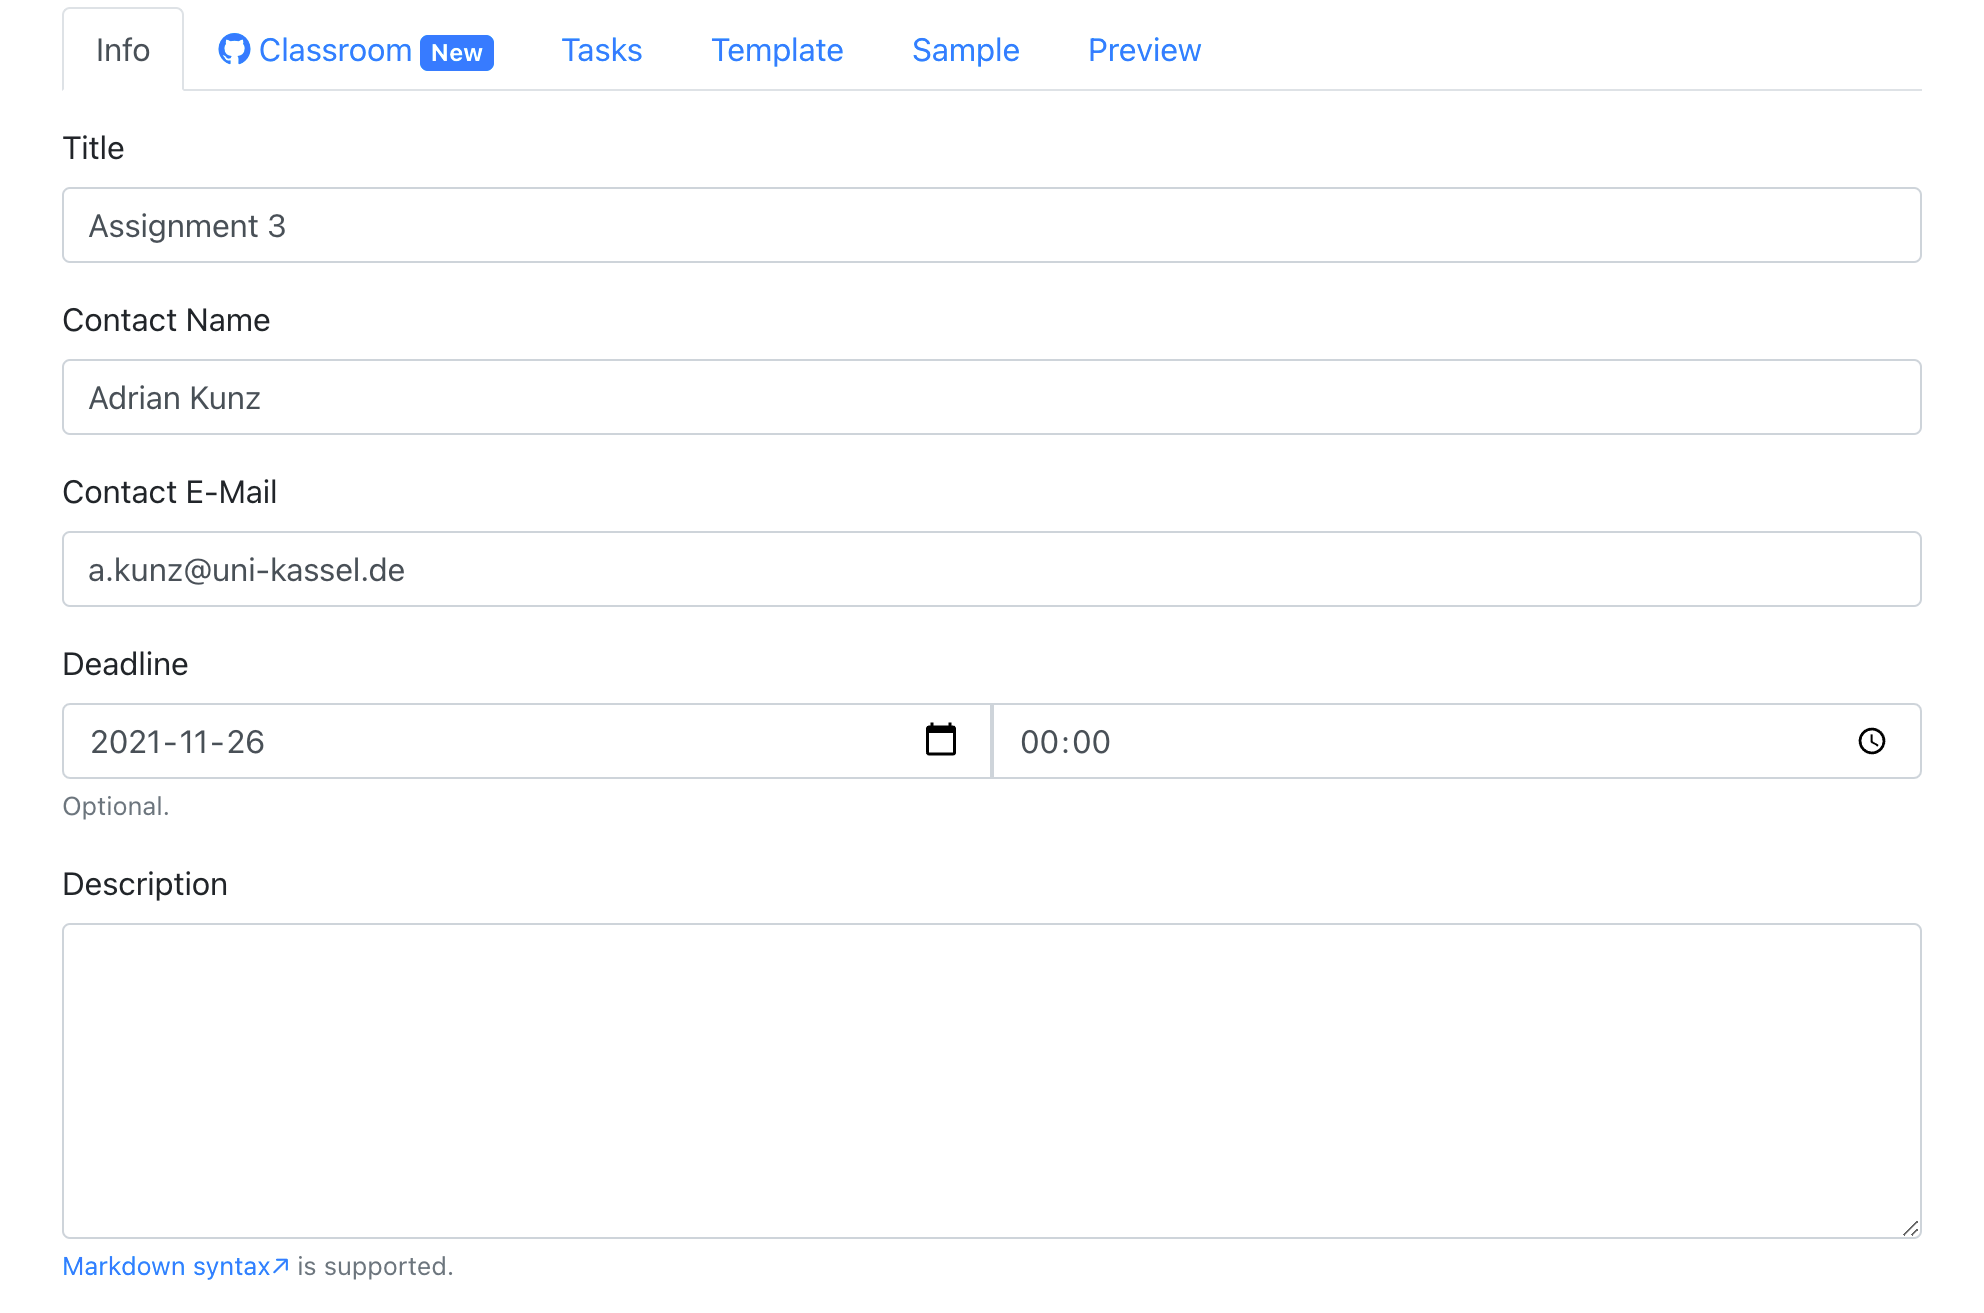
\includegraphics[width=\textwidth]{images/assignment-create-info}
    \caption{Formular für Rahmeninformationen eines Assignments}
    \label{fig:assignment-create-info}
\end{figure}

Zunächst werden einige Rahmeninformationen definiert.
Abbildung~\ref{fig:assignment-create-info} zeigt das zugehörige Formular.
Dazu gehören ein Titel (\textbf{Title}) für das Assignment, welcher der Zuordnung dient.
Ein Ansprechpartner, beispielsweise die Übungsleitung, und dessen Email-Adresse werden in den Feldern \textbf{Contact Name} und \textbf{Contact Email} festgelegt.
Die optionale Abgabefrist (\textbf{Deadline}) hat zwei wesentliche Verwendungszwecke.
Einerseits wird diese für den automatischen Import verwendet, der in Kürze anhand der GitHub Classroom-Integration erläutert wird.
Andererseits kann anhand der Deadline dargestellt werden, welche Lösungen zu spät eingereicht wurden.
Ein Beispiel dafür wird in Abschnitt~\ref{subsec:grading} gezeigt.
Die Beschreibung (\textbf{Description}) kann weitere Informationen über das Assignment enthalten, wird aber nachfolgend nicht verwendet.

\begin{figure}
    \centering
    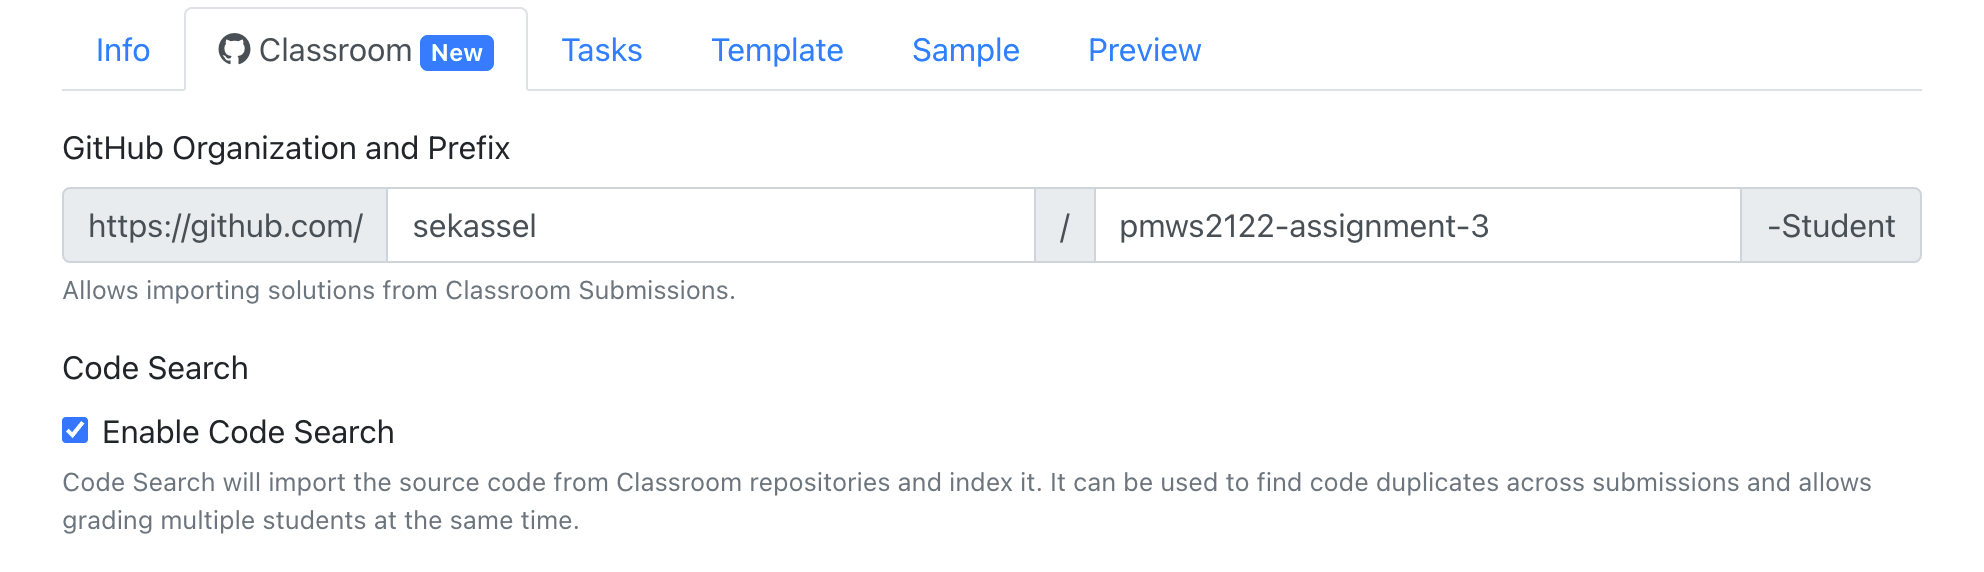
\includegraphics[width=\textwidth]{images/assignment-create-classroom}
    \caption{Formular für GitHub Classroom-Einstellungen eines Assignments}
    \label{fig:assignment-create-classroom}
\end{figure}

Auf der nächsten Seite des Formulars können Angaben für die GitHub Classroom-Integration gemacht werden.
Abbildung~\ref{fig:assignment-create-classroom} zeigt ein Bild dieses Formulars.
Dafür müssen der Name der GitHub-Organisation (\textbf{Organization}) und das Präfix (\textbf{Prefix}) konfiguriert werden.
Dies ermöglicht die manuelle oder zum Zeitpunkt der Deadline automatische Importierung von Lösungen von der Platform.
Anhand der Search-\ac{api} von GitHub\footnote{\url{https://docs.github.com/en/rest/reference/search\#search-repositories}} wird nach allen Repositories in der angegebenen Organisation gesucht, deren Name mit dem Präfix beginnt.
Damit private Repositories in der Organisation gefunden werden können, muss das \textbf{GitHub Token} angegeben werden.
Der Hilfetext des Eingabefelds gibt Auskunft darüber, wie dieses erstellt werden kann.
Aus dem Repository-Name ohne Präfix kann der GitHub-Benutzername des Studierenden ermittelt werden, der für die Zuordnung der Lösung verwendet wird.
In Abschnitt~\ref{subsec:grading} ist ein Beispiel für die entstehende Lösungstabelle sichtbar.
Weiterhin wird das neueste Commit zum Zeitpunkt des Imports gespeichert, um die Reproduzierbarkeit einer Bewertung zu gewährleisten.
Insbesondere wird dadurch sichergestellt, dass Studierende ihre Lösungen nicht verfälschen, indem sie Änderungen am Quellcode nach Ablauf der Abgabefrist durchführen oder hochladen.
Anhand des Commits kann der exakte Stand zum Zeitpunkt der Abgabefrist wiederhergestellt werden.
Ist der Haken \textbf{Code Search} gesetzt, werden neben dem Commit auch die Dateien des Repositories heruntergeladen und separat gespeichert.
Diese dienen nicht der Reproduzierbarkeit, sondern der Textsuche, wie in Abschnitt~\ref{subsec:code-search} näher erläutert wird.
Aus diesem Grund wird auch kein Anspruch auf Vollständigkeit der Daten gestellt.
Vergleichsweise große Dateien (> 64KB) werden nicht gespeichert, da gewöhnliche Quellcode-Dateien aus Hausaufgaben-Lösungen diese Größe nicht überschreiten.\footnote{
    Die Suche nach Quelltext-Dateien größer als 64KB in der GitHub-Organisation "sekassel" ergab lediglich Ergebnisse aus Node.js-Projekten, darunter primär \code{package-lock.json}-Dateien und Dateien in versehentlich gepushten \code{node_modules}-Ordnern.
    Da dies generierter \ac{bzw} von Drittanbietern stammender Code ist, handelt es sich nicht um relevante Teile der Lösung, die durchsucht werden müssten.
}

\begin{figure}
    \centering
    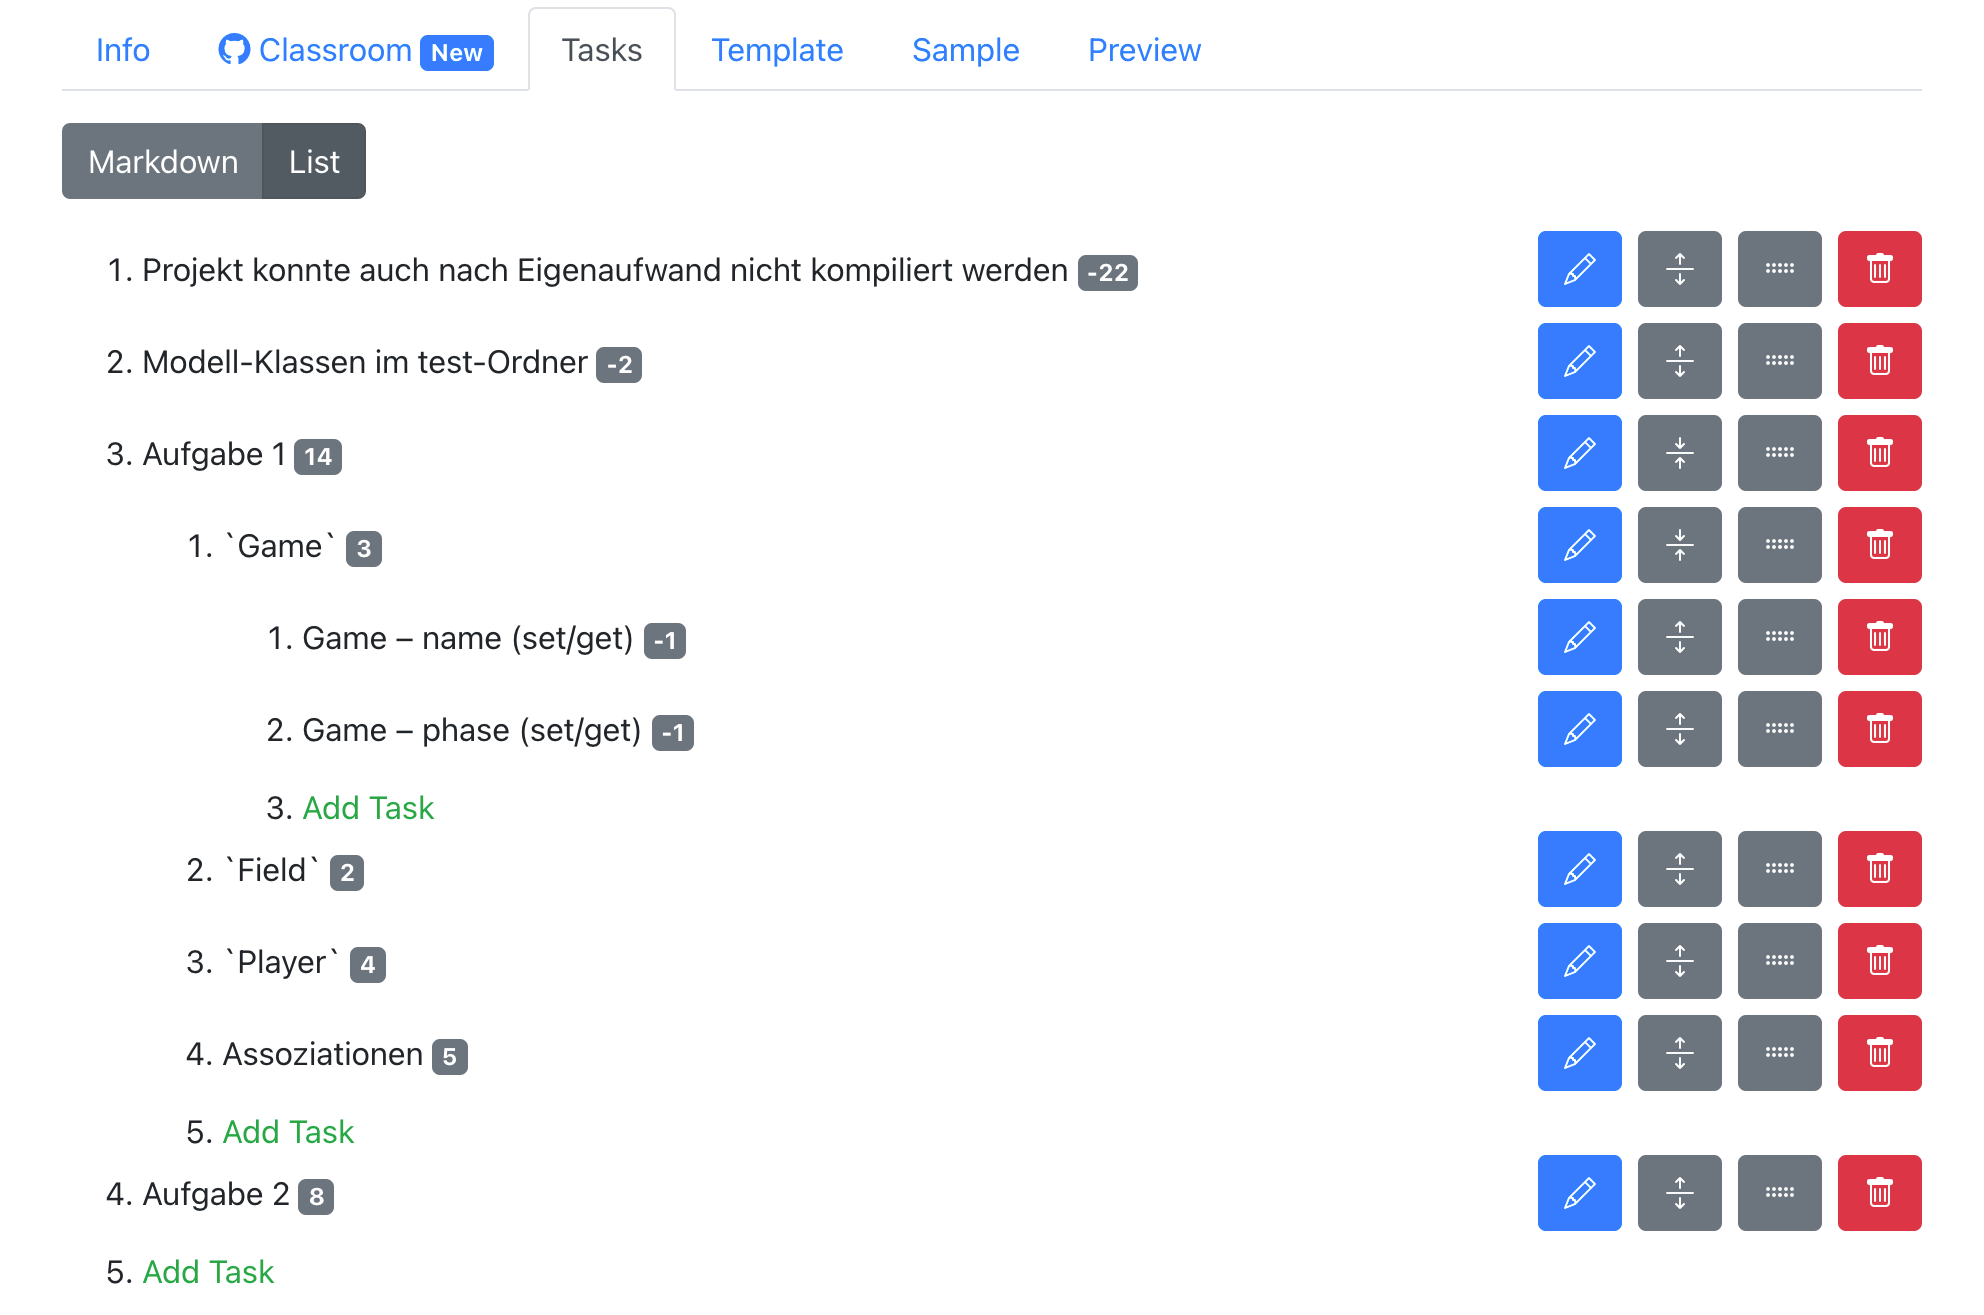
\includegraphics[width=\textwidth]{images/assignment-create-tasks-list}
    \caption{Baum-Editor für Teilaufgaben}
    \label{fig:assignment-create-tasks-list}
\end{figure}

Nun muss die Struktur des Aufgabenblatts anhand von Teilaufgaben, genannt Tasks, definiert werden.
Diese können beliebig geschachtelt und angeordnet werden, weshalb ein spezieller Editor für die Bearbeitung notwendig ist.
Abbildung~\ref{fig:assignment-create-tasks-list} zeigt, wie dieser in der Oberfläche aussieht.
Jeder Task besteht mindestens aus einer kurzen Beschreibung, die auch als Titel dienen kann, und einer Punktzahl.
In der Abbildung ist bereits erkennbar, dass eine Punktzahl nicht zwangsweise positiv sein muss.
Ein Task mit negativer Punktzahl wird als Abzug bezeichnet und kann besonders dann eingesetzt werden, wenn eine Aufgabe aus vielen ungeordneten Teilen besteht.
Dann ist es möglich, in einem Feedback nur die zutreffenden Abzüge darzustellen und damit die Übersichtlichkeit und Nachvollziehbarkeit zu verbessern.

Neben jedem Task werden vier Buttons angezeigt.
Der blaue Stift öffnet die Detailansicht des Tasks, die in den Abbildungen~\ref{fig:assignment-create-tasks-detail} dargestellt ist und im Folgenden beschrieben wird.
Mit dem Pfeile-Button kann ein Task aus- oder eingeklappt werden, um die Untertasks anzuzeigen oder zu verbergen.
Die nächste Schaltfläche kann verwendet werden, um die Reihenfolge der Tasks anzupassen oder Tasks unter andere zu verschieben.
Zuletzt erlaubt der Mülleimer-Button das Löschen eines Tasks.
Dabei handelt es sich nicht um eine sofortige Löschung, der Task wird lediglich als gelöscht markiert und kann wiederhergestellt werden, um eventuellen Datenverlust zu vermeiden.

\begin{figure}
    \centering
    \begin{subfigure}[t]{0.475\textwidth}
        \centering
        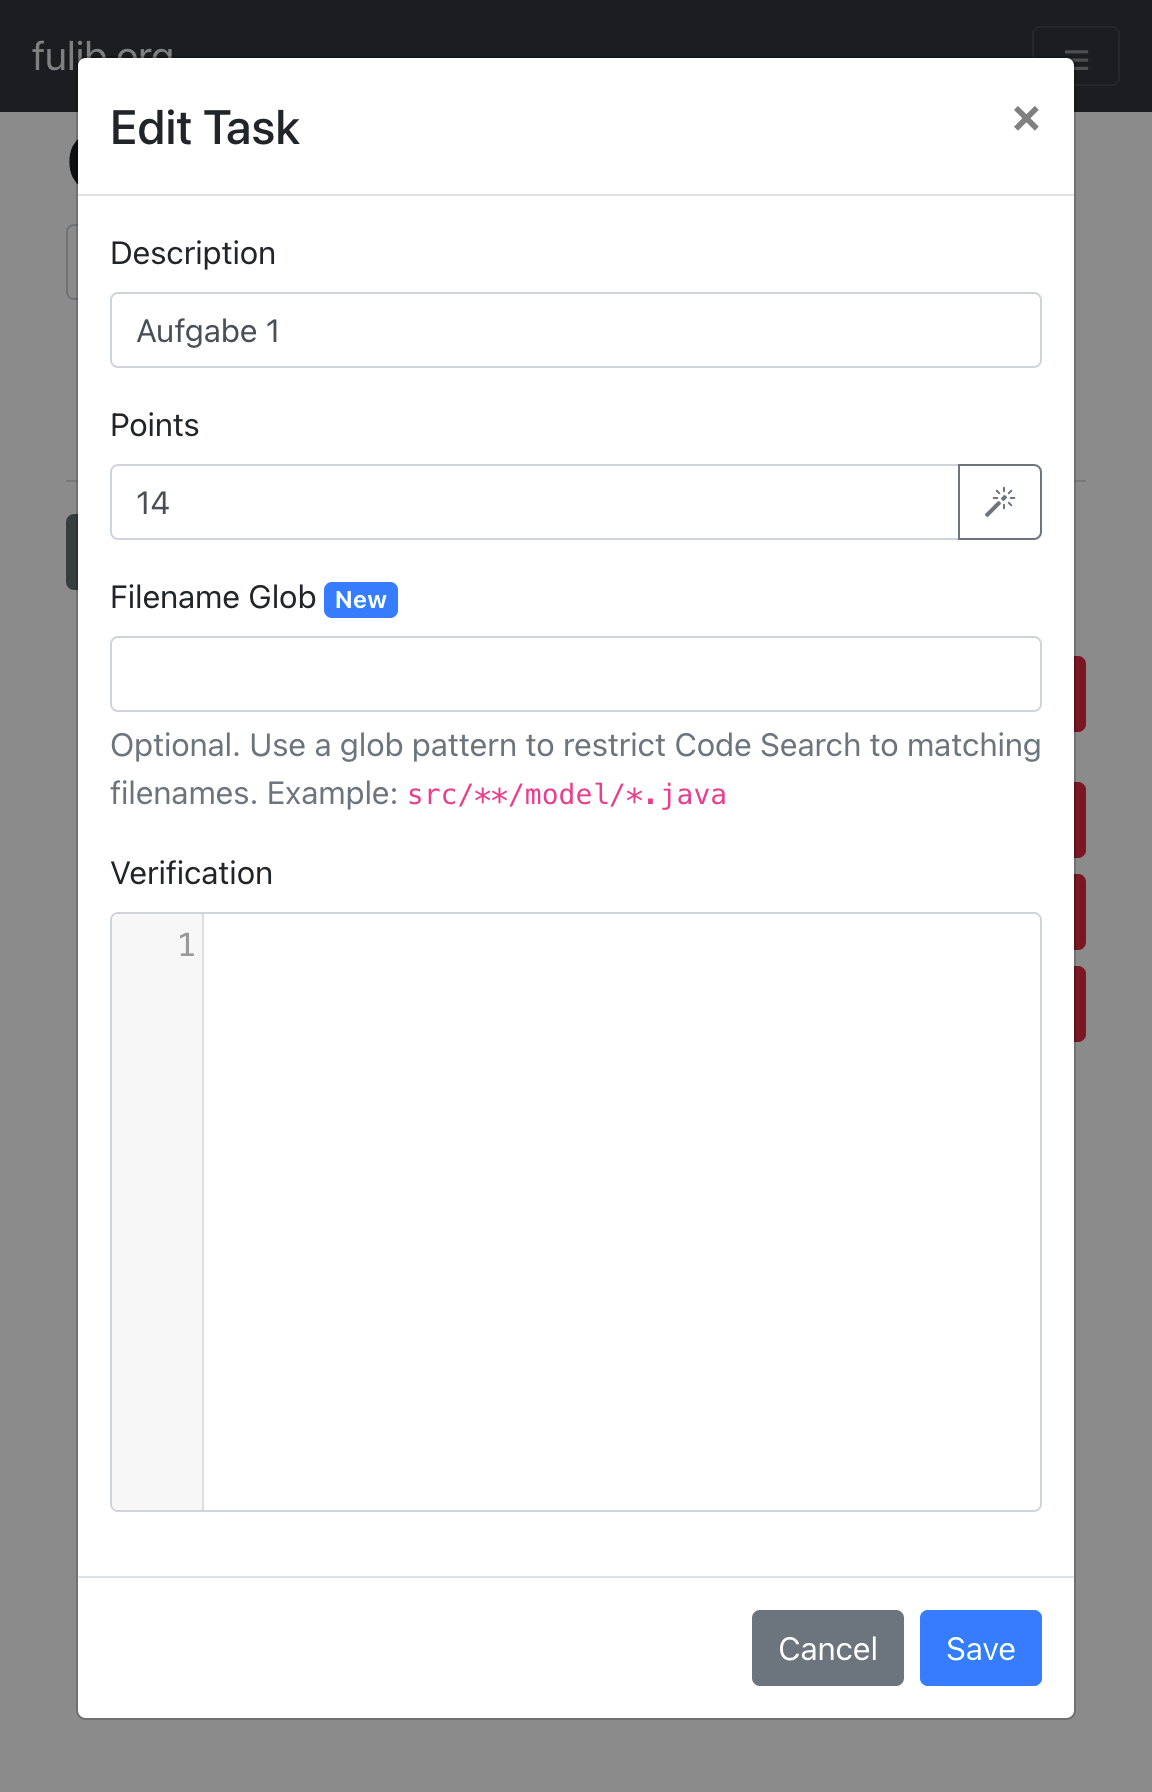
\includegraphics[width=\textwidth]{images/assignment-create-tasks-detail-1}
        \caption{Detailansicht eines positiven Tasks mit Untertasks}
        \label{fig:assignment-create-tasks-detail-1}
    \end{subfigure}
    \hfill
    \begin{subfigure}[t]{0.475\textwidth}
        \centering
        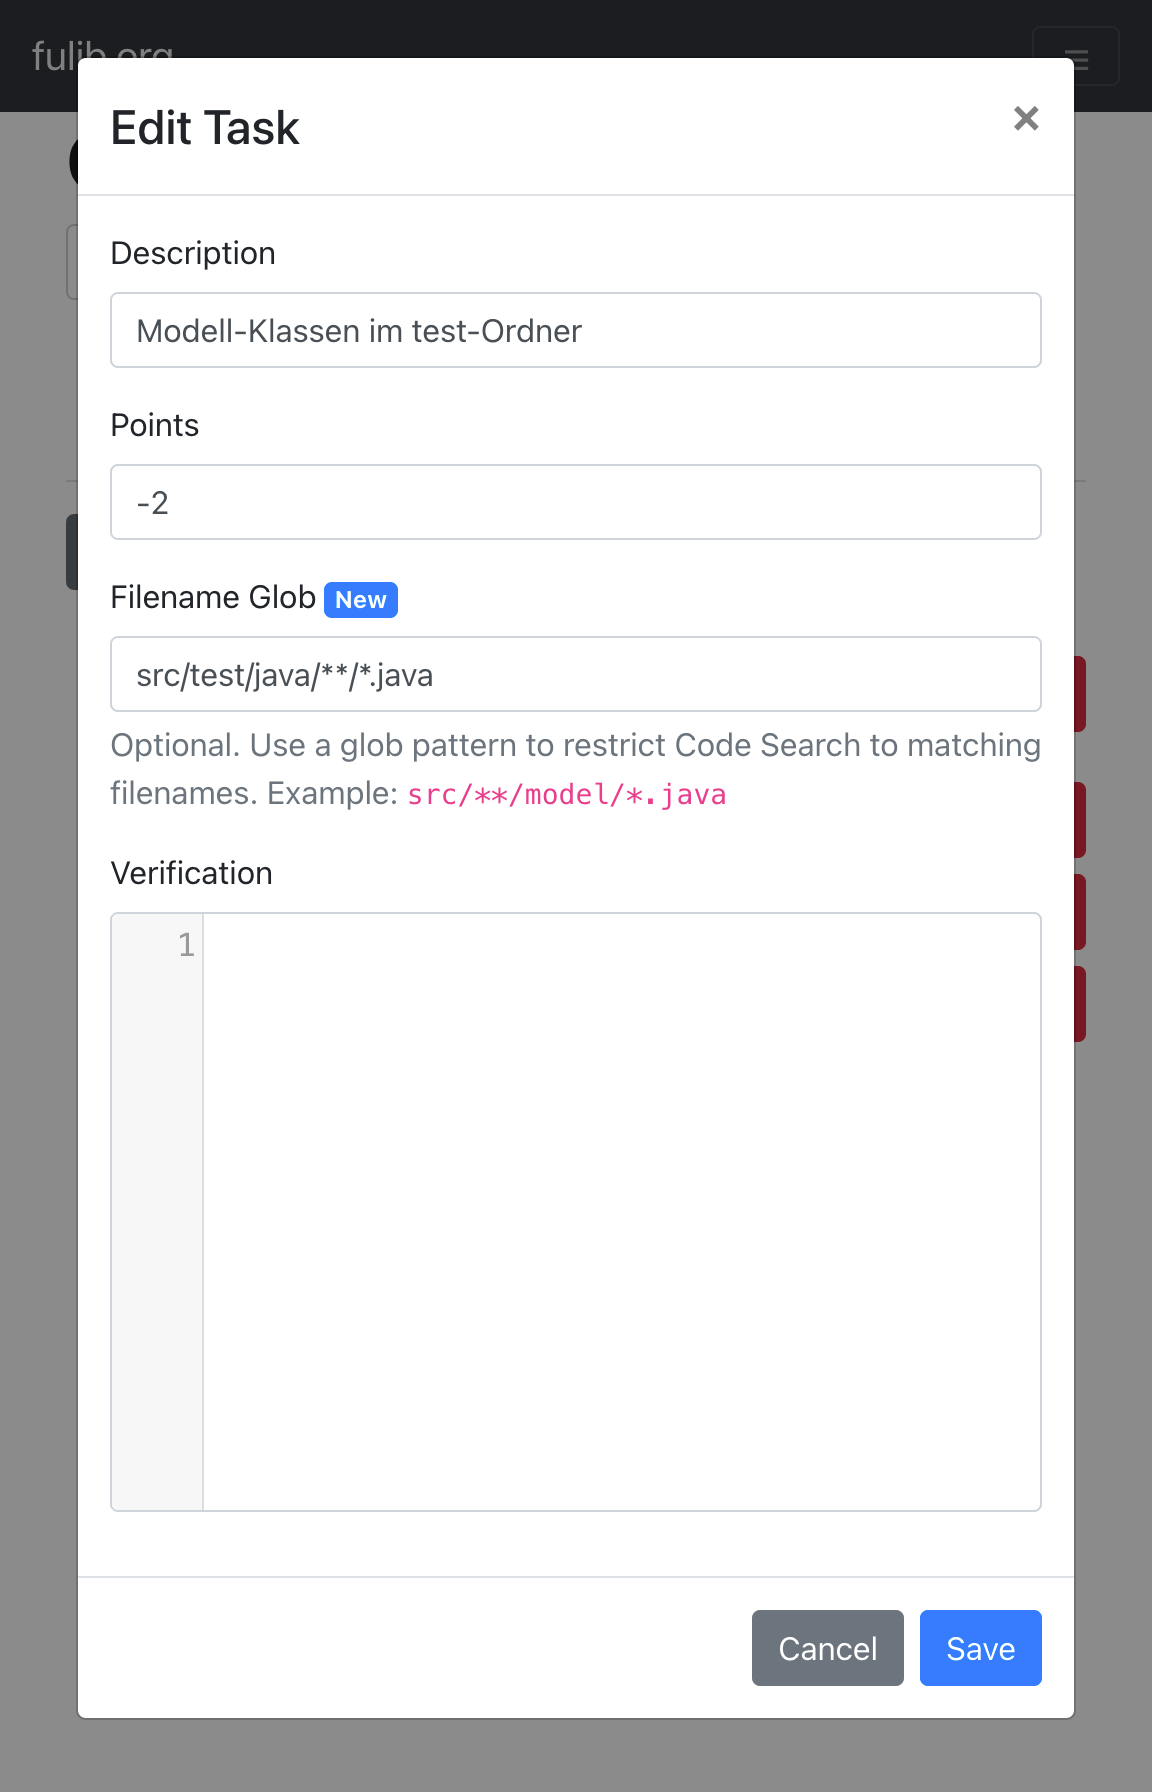
\includegraphics[width=\textwidth]{images/assignment-create-tasks-detail-2}
        \caption{Detailansicht eines negativen Tasks}
        \label{fig:assignment-create-tasks-detail-2}
    \end{subfigure}
    \caption{Detailansicht zweier Tasks}
    \label{fig:assignment-create-tasks-detail}
\end{figure}

Die Detailansichten eines positiven Tasks mit Untertasks und eines negativen Tasks sind jeweils in den Abbildungen~\ref{fig:assignment-create-tasks-detail-1} und~\ref{fig:assignment-create-tasks-detail-2} sichtbar.
In dem modalen Formular kann die Beschreibung und die Punktzahl eingestellt werden.
In der ersten Abbildung ist zu sehen, dass die Existenz von Unteraufgaben die automatische Berechnung der Punktzahl ermöglicht, weshalb der Zauberstab-Button neben dem Eingabefeld sichtbar ist.
Die Berechnung behandelt Unteraufgaben mit negativen Punktzahlen gesondert, indem jeweils deren absoluter Betrag verwendet wird.
Das optionale Eingabefeld \textbf{Filename Glob} ist für die in Abschnitt~\ref{subsec:code-search} beschriebene Code Search relevant und wird dort separat beschrieben.
Abbildung~\ref{fig:assignment-create-tasks-detail-2} zeigt eine Beispieleingabe.
Der Editor \textbf{Verification} wird für die automatische Bewertung mit fulibScenarios und dessen Pattern Matching-Erweiterung aus~\cite{bachelor-thesis} verwendet und ist in dieser Arbeit nicht weiter relevant.

\begin{figure}
    \centering
    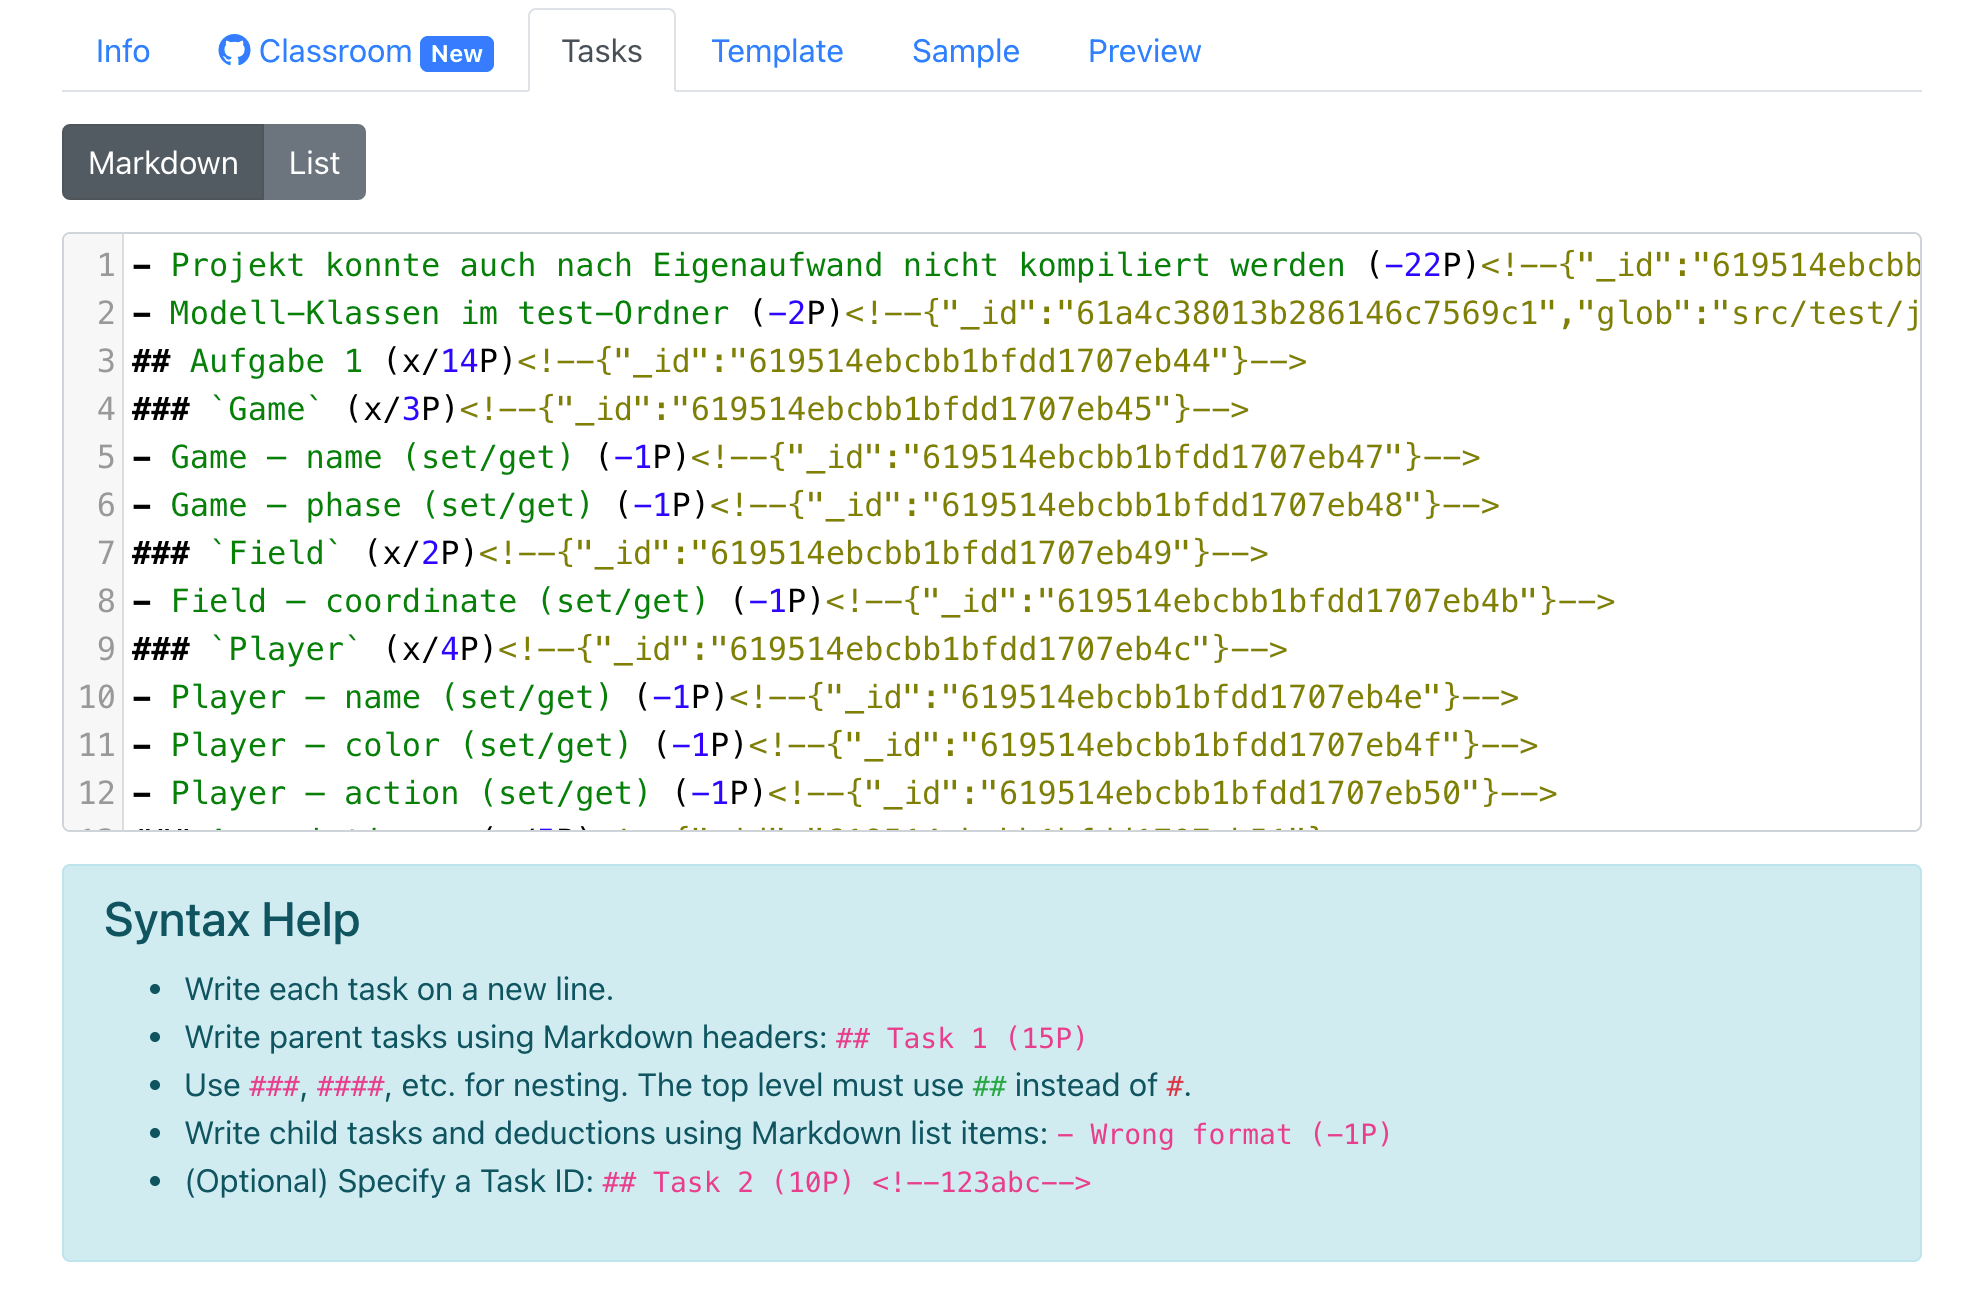
\includegraphics[width=\textwidth]{images/assignment-create-tasks-markdown}
    \caption{Markdown-Editor für Teilaufgaben}
    \label{fig:assignment-create-tasks-markdown}
\end{figure}

Die Schaltfläche zum Wechseln zwischen \textbf{Markdown} und \textbf{List} erlaubt die Bearbeitung der Tasks in einer auf Markdown basierenden Textformat.
Abbildung~\ref{fig:assignment-create-tasks-markdown} zeigt einen Ausschnitt der Teilaufgabenliste aus Abbildung~\ref{fig:assignment-create-tasks-list} in diesem Format sowie der zugehörige Hilfetext zur Erklärung.
Das Format kann in wenigen Sätzen beschrieben werden.
Jeder Task wird in eine neue Zeile geschrieben, die entweder der Listensyntax (\code{-} am Anfang) oder der Überschriftensyntax (Zwei oder mehrere \code{\#} am Anfang) von Markdown folgt.
Nach dem einleitenden Zeichen folgt die Beschreibung und die Punktzahl, optional mit \code{x/} vorangestellt und/oder \code{P} nachgestellt, in Klammern.
Am Ende der Zeile kann ein \ac{html}-Kommentare weitere Daten des Tasks wie dessen \ac{id} und Dateinamen-Glob in \ac{json} kodiert enthalten.
Folgt eine Zeile nicht diesem Format, wird sie rot markiert, um den Benutzer auf das Problem hinzuweisen.

Das Format wurde gewählt, da die Bewertungsrichtlinien der Veranstaltung Programmieren und Modellieren bereits vor Beginn dieser Arbeit in ähnlichem Format vorlagen.
Diese Richtlinien haben ihre Ursprünge aus der Verwendung von GitHub, wo Issues, Pull Requests und Kommentare in Markdown verfasst werden können und dann in Listenform mit Teilüberschriften dargestellt werden.
Meist war es während der Evaluation möglich, die Bewertungsrichtlinien einzusetzen und mit wenigen Änderungen dem Format anzupassen.

Die Registerkarten \textbf{Template} und \textbf{Sample} aus Abbildung~\ref{fig:assignment-create-head} werden an dieser Stelle nicht näher erläutert.
Es handelt sich um spezifische Einstellungen für die Bewertung von Szenarien aus~\cite{bachelor-thesis}, die für die Zwecke dieser Arbeit nicht anwendbar sind.

\begin{figure}
    \centering
    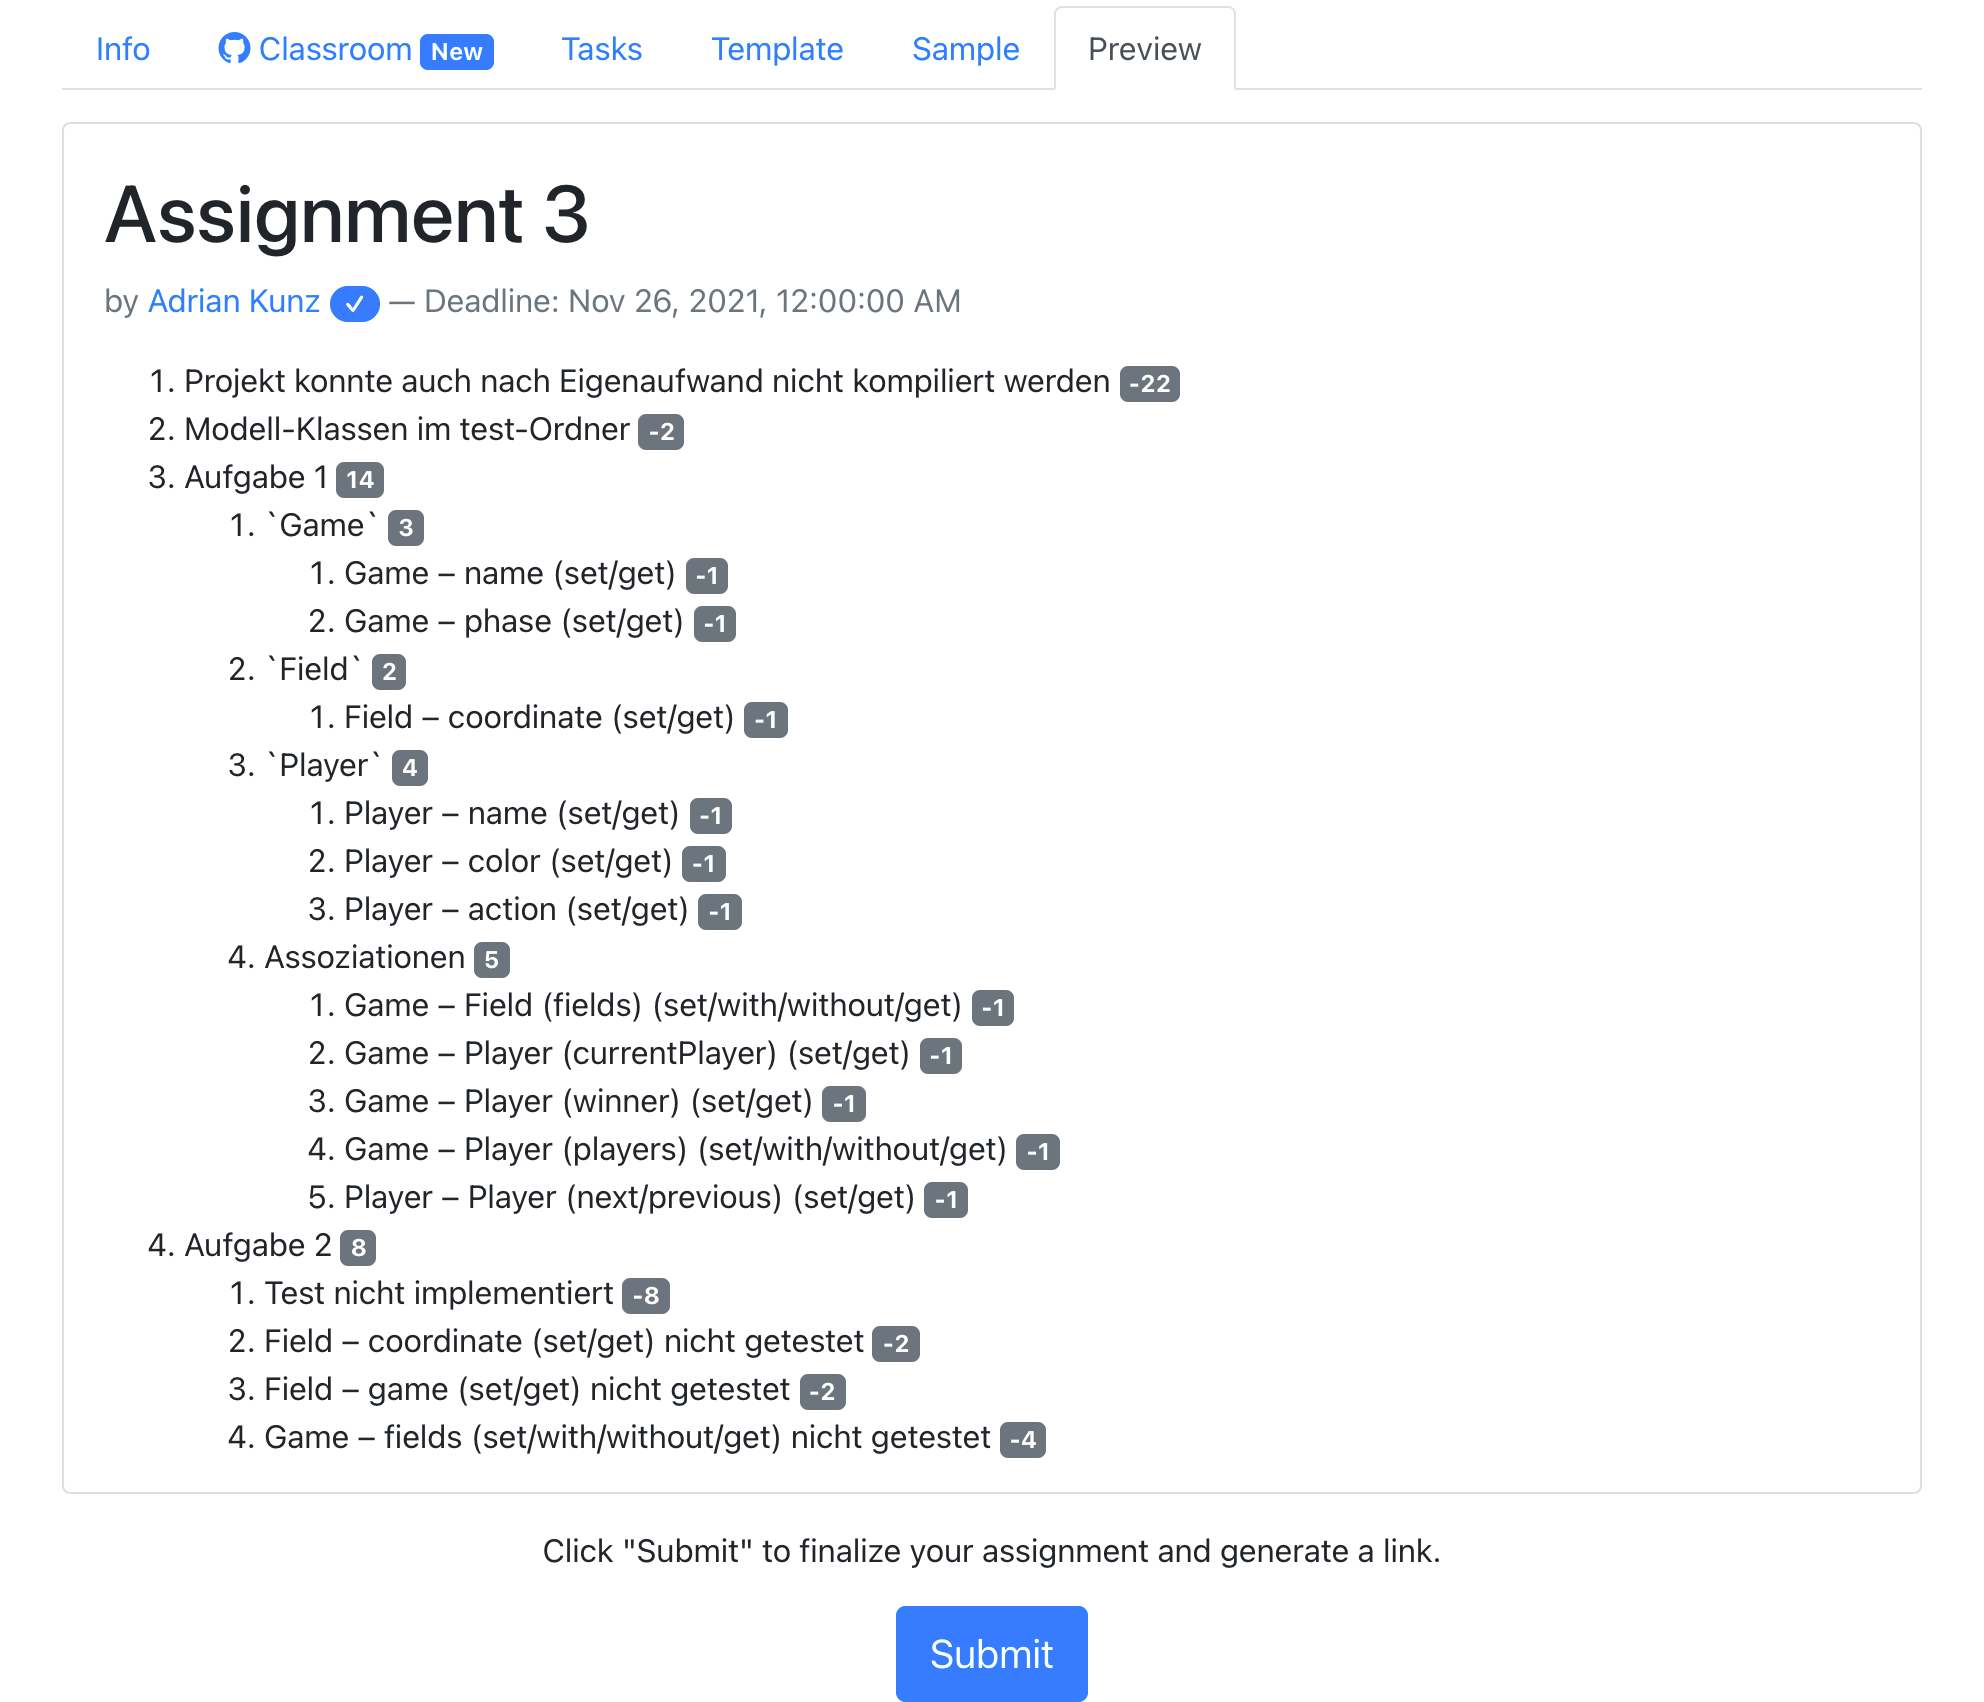
\includegraphics[width=\textwidth]{images/assignment-create-preview}
    \caption{Abschließende Vorschau vor Erstellen eines Assignments}
    \label{fig:assignment-create-preview}
\end{figure}

Der letzte Schritt der Assignment-Erstellung befindet sich auf der Registerkarte \textbf{Preview}, welche eine Übersicht über das Assignment anhand einer Vorschau anzeigt.
In Abbildung~\ref{fig:assignment-create-preview} wird diese dargestellt.
In der Vorschau werden Titel, Autor, Abgabefrist und, falls vorhanden, die Beschreibung angezeigt.
Sämtliche Teilaufgaben werden in einer geschachtelten Liste mit Beschreibung und Punktzahl präsentiert.
Schließlich kann das Assignment mit dem \textbf{Submit}-Button erstellt und veröffentlicht werden.

\begin{figure}
    \centering
    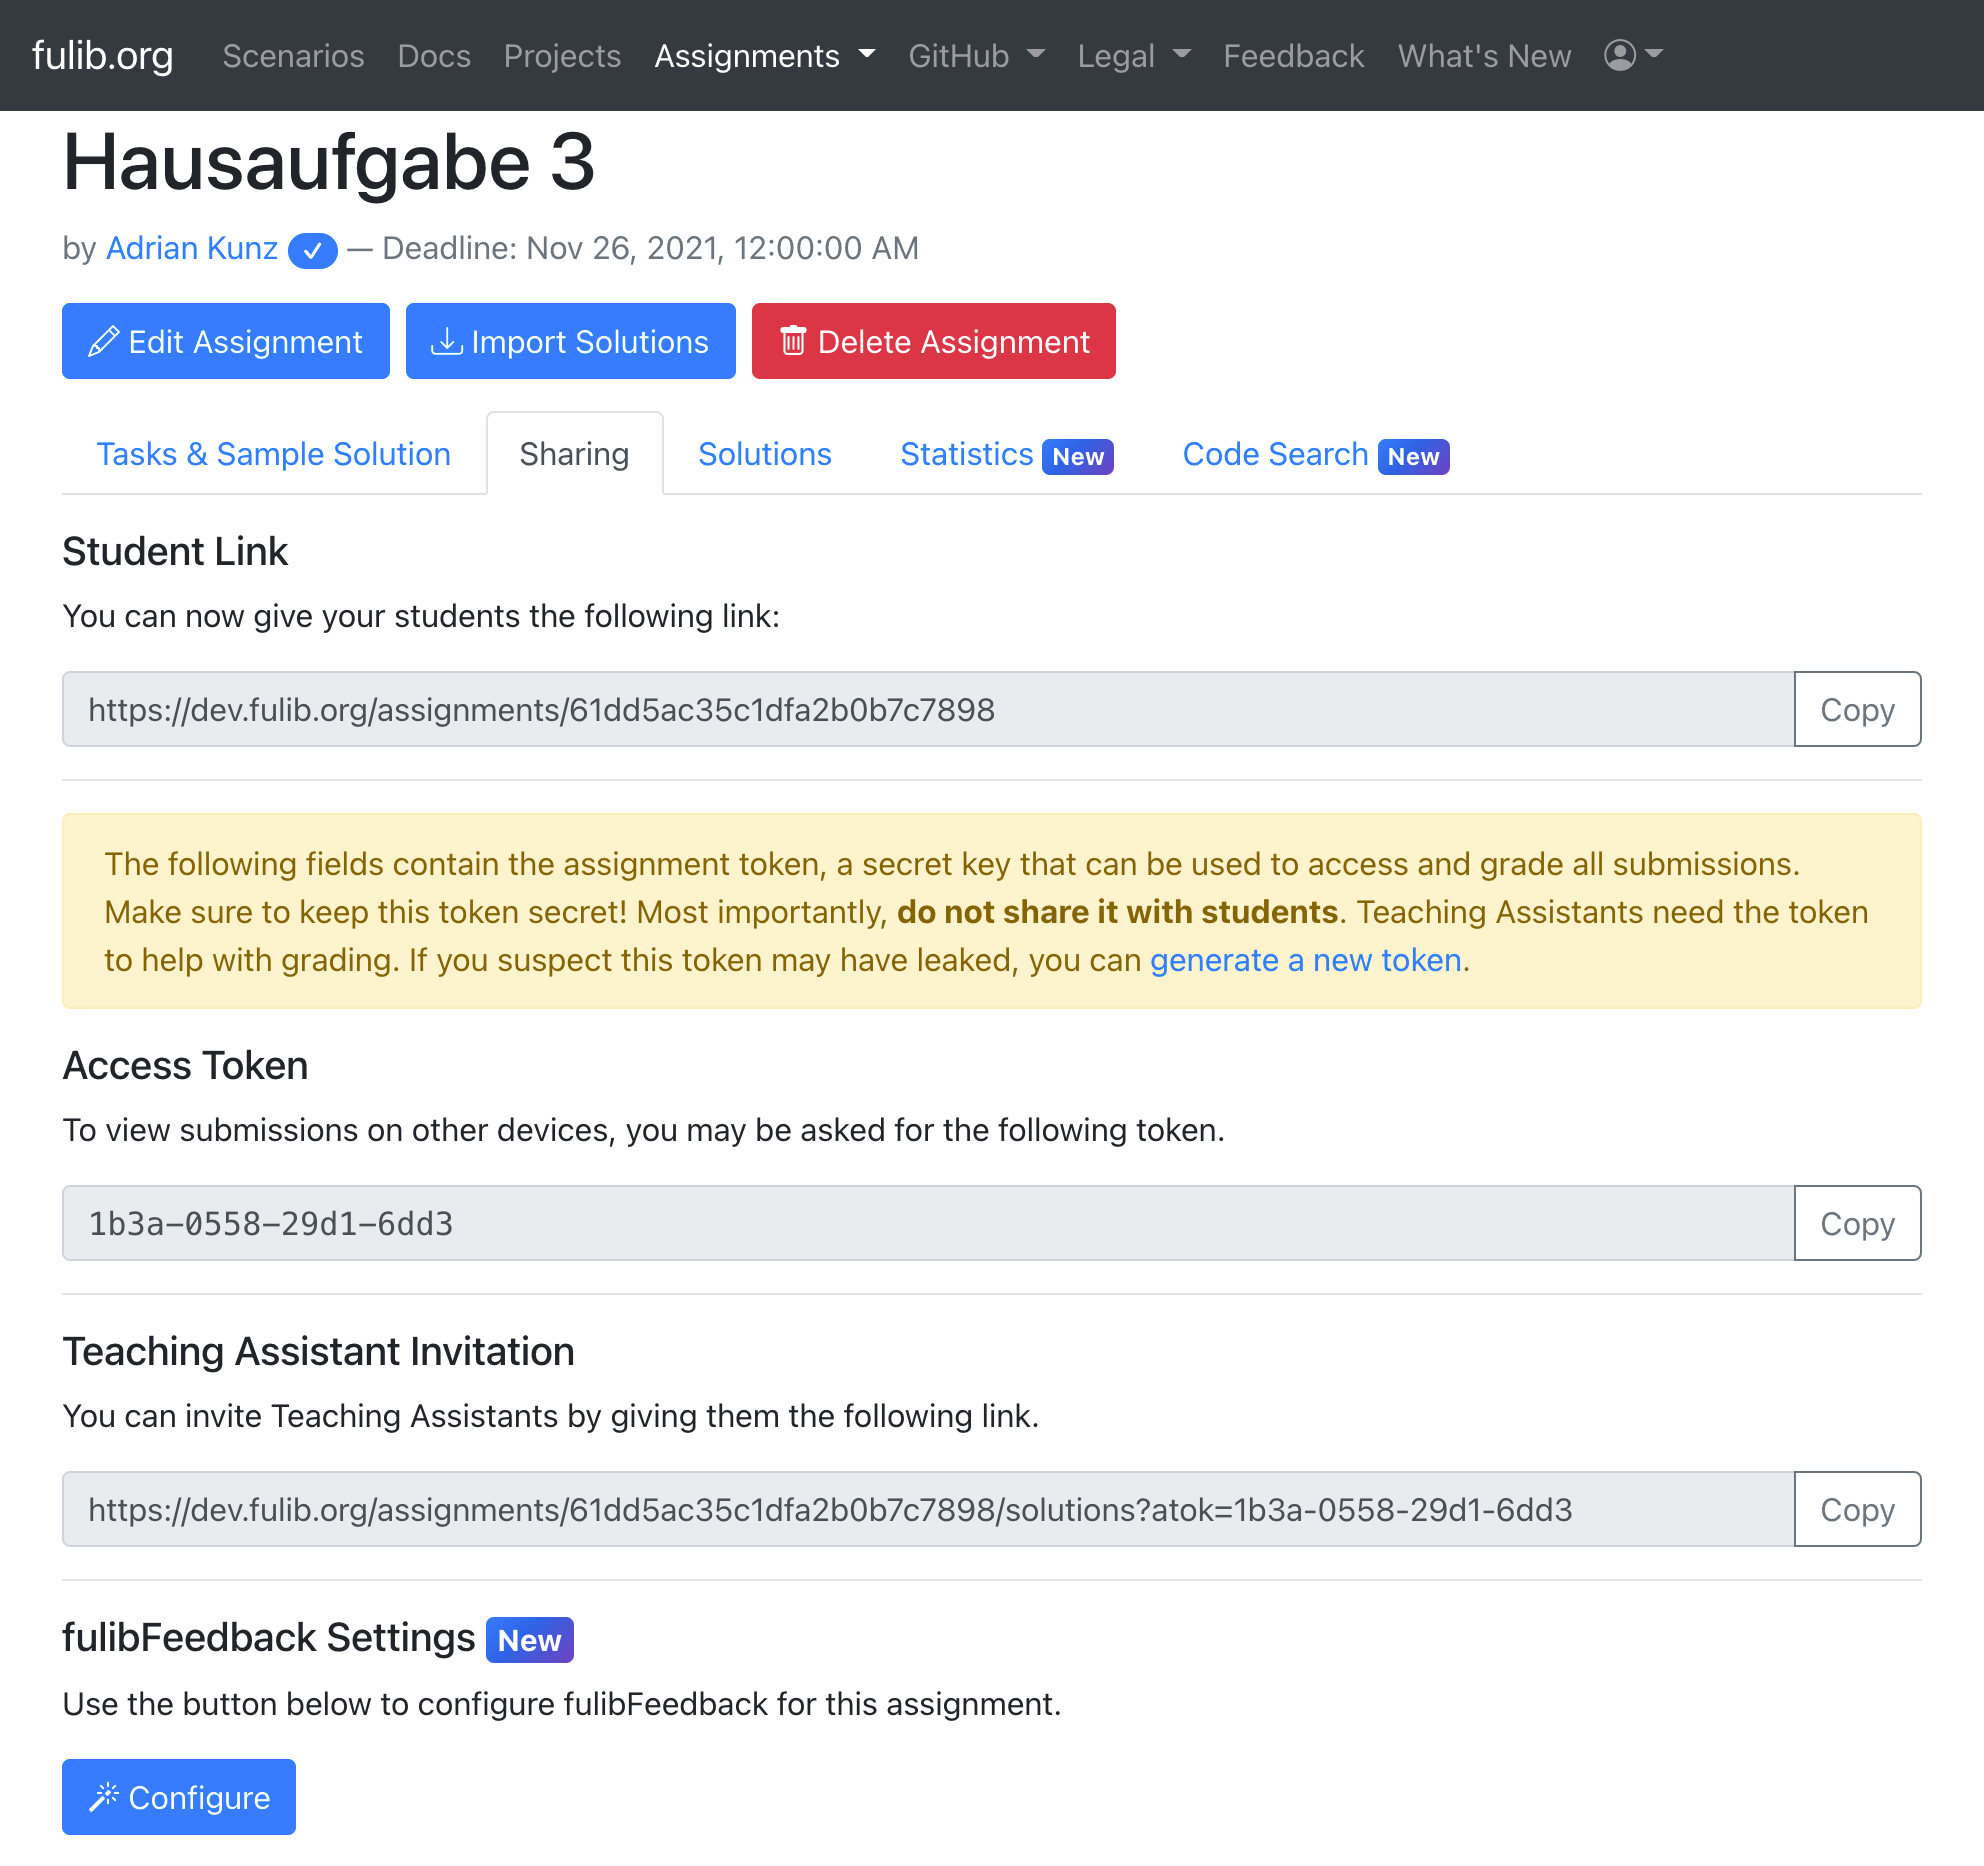
\includegraphics[width=\textwidth]{images/assignment-share}
    \caption{Teilen eines Assignments}
    \label{fig:assignment-share}
\end{figure}

Die Veröffentlichung findet über den \textbf{Sharing}-Tab statt, der sich direkt nach Erstellen des Assignments öffnet und in Abbildung~\ref{fig:assignment-share} dargestellt ist.
Der \textbf{Student Link} wurde hauptsächlich in~\cite{bachelor-thesis} eingesetzt, da dieser zur Vergabe an die Studierenden vorgesehen war.
In dieser Arbeit interagieren diese jedoch nicht mit der Oberfläche, weshalb der Link nicht benötigt wird.
Das \textbf{Access Token} dient der Zugriffskontrolle, da mit diesem sämtliche Aktionen von Bewertenden durchgeführt werden.
Daher muss sichergestellt werden, dass es nicht an Studierende gelangt, wie die Warnmeldung beschreibt.
Bewertende benötigen folglich das Token und können es über den teilbaren \textbf{Teaching Assistant Invitation}-Link erhalten.
Der Button \textbf{Configure} wird für fulibFeedback eingesetzt und wird in Abschnitt~\ref{sec:fulibFeedback} erneut erwähnt.

\subsection{Bewertung}\label{subsec:grading}

Sobald die Bewertenden den Einladungslink für ein Assignment erhalten haben, können sie mit der Bewertung beginnen.
Nachfolgend werden einige Schritte beschrieben, die dafür notwendig sind.
Es handelt sich um wiederholende Abläufe, die jedoch nach kurzer Eingwöhnungszeit eine effiziente Arbeitsweise erlauben.
Dies wird in Kapitel~\ref{ch:evaluation} näher beleuchtet.

\subsubsection{Abgabentabelle}

Begonnen wird in der Tabelle mit allen Abgaben unter dem Tab \textbf{Solutions}.
Diese ist in Abbildung~\ref{fig:assignment-solutions-table} ausgeschnitten dargestellt.

\begin{figure}
    \centering
    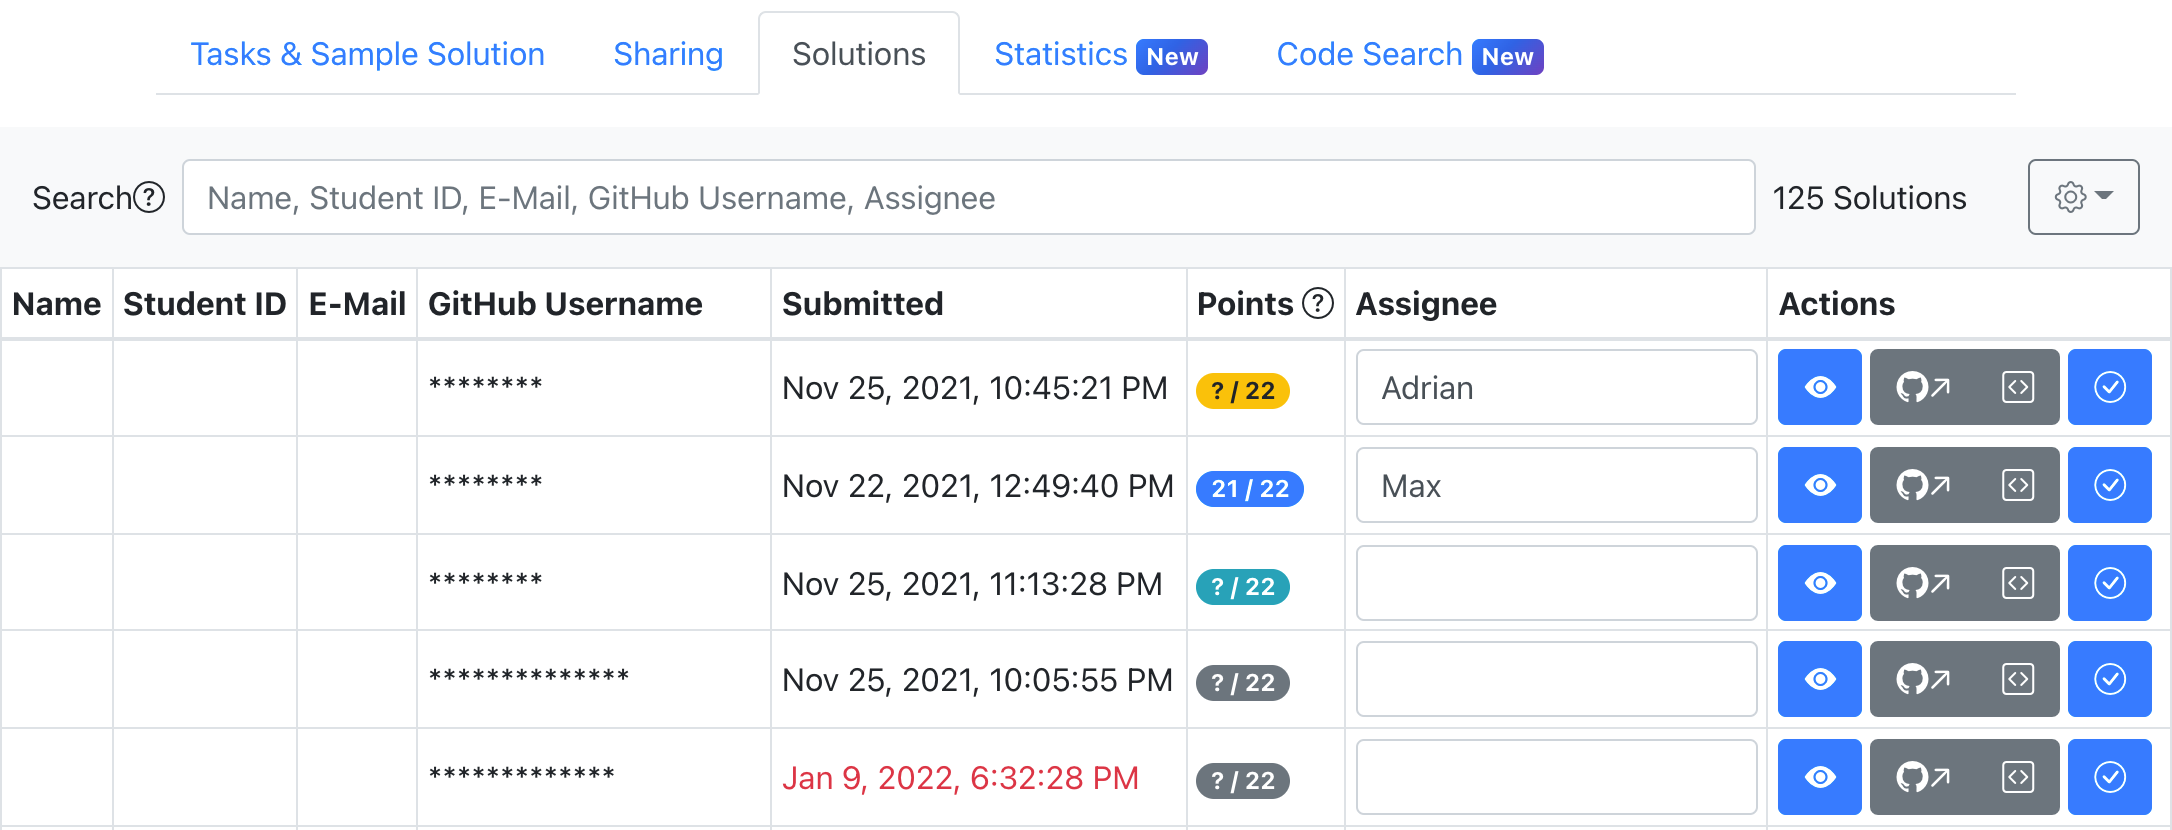
\includegraphics[width=\textwidth]{images/assignment-solutions-table}
    \caption{Tabelle mit allen Abgaben nach dem Import}
    \label{fig:assignment-solutions-table}
\end{figure}

In diesem Fall wurden die Lösungen automatisch nach Ablauf der Abgabefrist aus dem GitHub Classroom importiert.
Die Tabelle gibt Auskunft über den GitHub-Benutzernamen\footnote{Für diese Abbildung wurden die Benutzernamen durch \texttt{*}-Symbole ersetzt.} und das Abgabedatum (\textbf{Submitted}), welches dem letzten Push\footnote{Bezeichnet die Aktion der Versionskontroll-Software Git, bei der lokale Commits auf den Remote-Server hochgeladen werden.}-Zeitpunkt vor der Frist entspricht.
Bei einem nachträglichen manuellem Import ist es möglich, dass die Push-Zeit nach der Abgabefrist liegt.
In diesem Fall wird das Abgabedatum rot markiert.
Name, Matrikelnummer (\textbf{Student ID}) und E-Mail-Adresse können nicht von GitHub Classroom ermittelt werden, weshalb sie in der Tabelle leer sind.

Die Punktzahl ist zunächst mit \texttt{?} als unausgewertet markiert.
In der Abbildung wurden bereits einige Bewertungen vorgenommen, weshalb die zweite Person eine abschließende Punktzahl von 21 erhalten hat.
Die gelb hinterlegte Punktzahl deutet an, dass eine Bewertung dieser Abgabe begonnen wurde, aber noch kein Feedback versendet wurde und daher keine Punktzahl feststeht.
Eine türkise Farbe markiert Abgaben, die zwar noch nicht händisch bewertet wurden, aber in denen eine automatisch angelegte Bewertung von Code Search vorhanden ist.
In Abgaben mit grauer Punktzahl ist keinerlei Bewertung vorhanden.
Das Fragezeichen-Symbol neben \textbf{Points} gibt Auskunft über diese Farbgebung.

Über die Textfelder unter \textbf{Assignee} können sich die Bewertenden die Abgaben zuordnen, für die sie zuständig sind.
Dadurch wird sichergestellt, dass nicht versehentlich eine Abgabe von mehreren Bewertenden betrachtet wird.
Die Textfelder bieten eine einfache Form der Autovervollständigung, sodass bei Eingabe weniger Buchstaben bereits der volle Name eines  Bewertenden vorgeschlagen wird, sofern dieser bereits an einer anderen Stelle eingetragen war.

Mit der Suchleiste kann die Tabelle nach verschiedenen Kriterien gefiltert werden.
Beispielsweise können Bewertende durch Eingabe ihres Namens nur die ihnen zugewiesenen Abgaben anzeigen, um für Übersicht zu sorgen.
Die Syntax der Suche ist komplexer als eine einfache Textsuche, weshalb das Fragezeichen-Symbol eine detaillierte Beschreibung der Syntax anzeigen kann.

Unter den \textbf{Actions} befinden sich die wichtigsten Aktionen, die für die Bewertung einer Abgabe relevant sind.
Mit dem Augen-Button kann die Detailansicht der Abgabe geöffnet werden, in der die Bewertung einzelner Teilaufgaben stattfindet.
Dies ist Inhalt des folgenden Abschnitts.
Der graue GitHub-Button öffnet das Repository, von dem die Lösung importiert wurde, auf GitHub und zeigt dabei den Stand des letzten Commits vor der Abgabefrist.
Der Button mit eingerahmten spitzen Klammern öffnet die Lösung sofort in einer \ac{ide}, indem das GitHub-Repository gecloned\footnote{Git-Bezeichnung für das Kopieren eines Online-Repositories in einen lokalen Ordner.} wird.
Mit dem Einstellungs-Button neben der Suchleiste kann zwischen verschiedenen \acp{ide} (\ac{vsc}, Code-OSS und VSCodium\footnote{Jeweils alternative quelloffene Builds von \ac{vsc} ohne Microsoft-Branding.}) und Clone-Protokollen (https und ssh) gewählt werden.
Der blaue Button mit eingekreistem Haken wird in einem späteren Abschnitt für das Versenden des Feedbacks verwendet.

\subsubsection{Abgabe-Detailansicht}

\begin{figure}
    \centering
    
\includegraphics[width=\textwidth]{images/solution-head}
    \caption{Kopf der Abgabe-Detailansicht}
    \label{fig:solution-head}
\end{figure}


Die Detailansicht einer Abgabe öffnet sich nach Klicken des Augen-Buttons in der Abgabetabelle.
In Abbildung~\ref{fig:solution-head} ist sichtbar, dass auch diese Ansicht wieder in mehrere Tabs aufgeteilt ist, um übersichtlich zu bleiben.
In der Kopfzeile wird der Name\footnote{Hier wurde der GitHub-Benutzername erneut durch \texttt{*}-Symbole ersetzt.} des Studierenden und die Abgabezeit stets angezeigt.
Für die Bewertung ist hauptsächlich der Tab \textbf{Solution \& Tasks} wichtig.
Die Teilaufgaben werden wieder in einer Baumansicht dargestellt, wie in Abbildung~\ref{fig:solution-tasks} erkennbar ist.

\begin{figure}
    \centering
    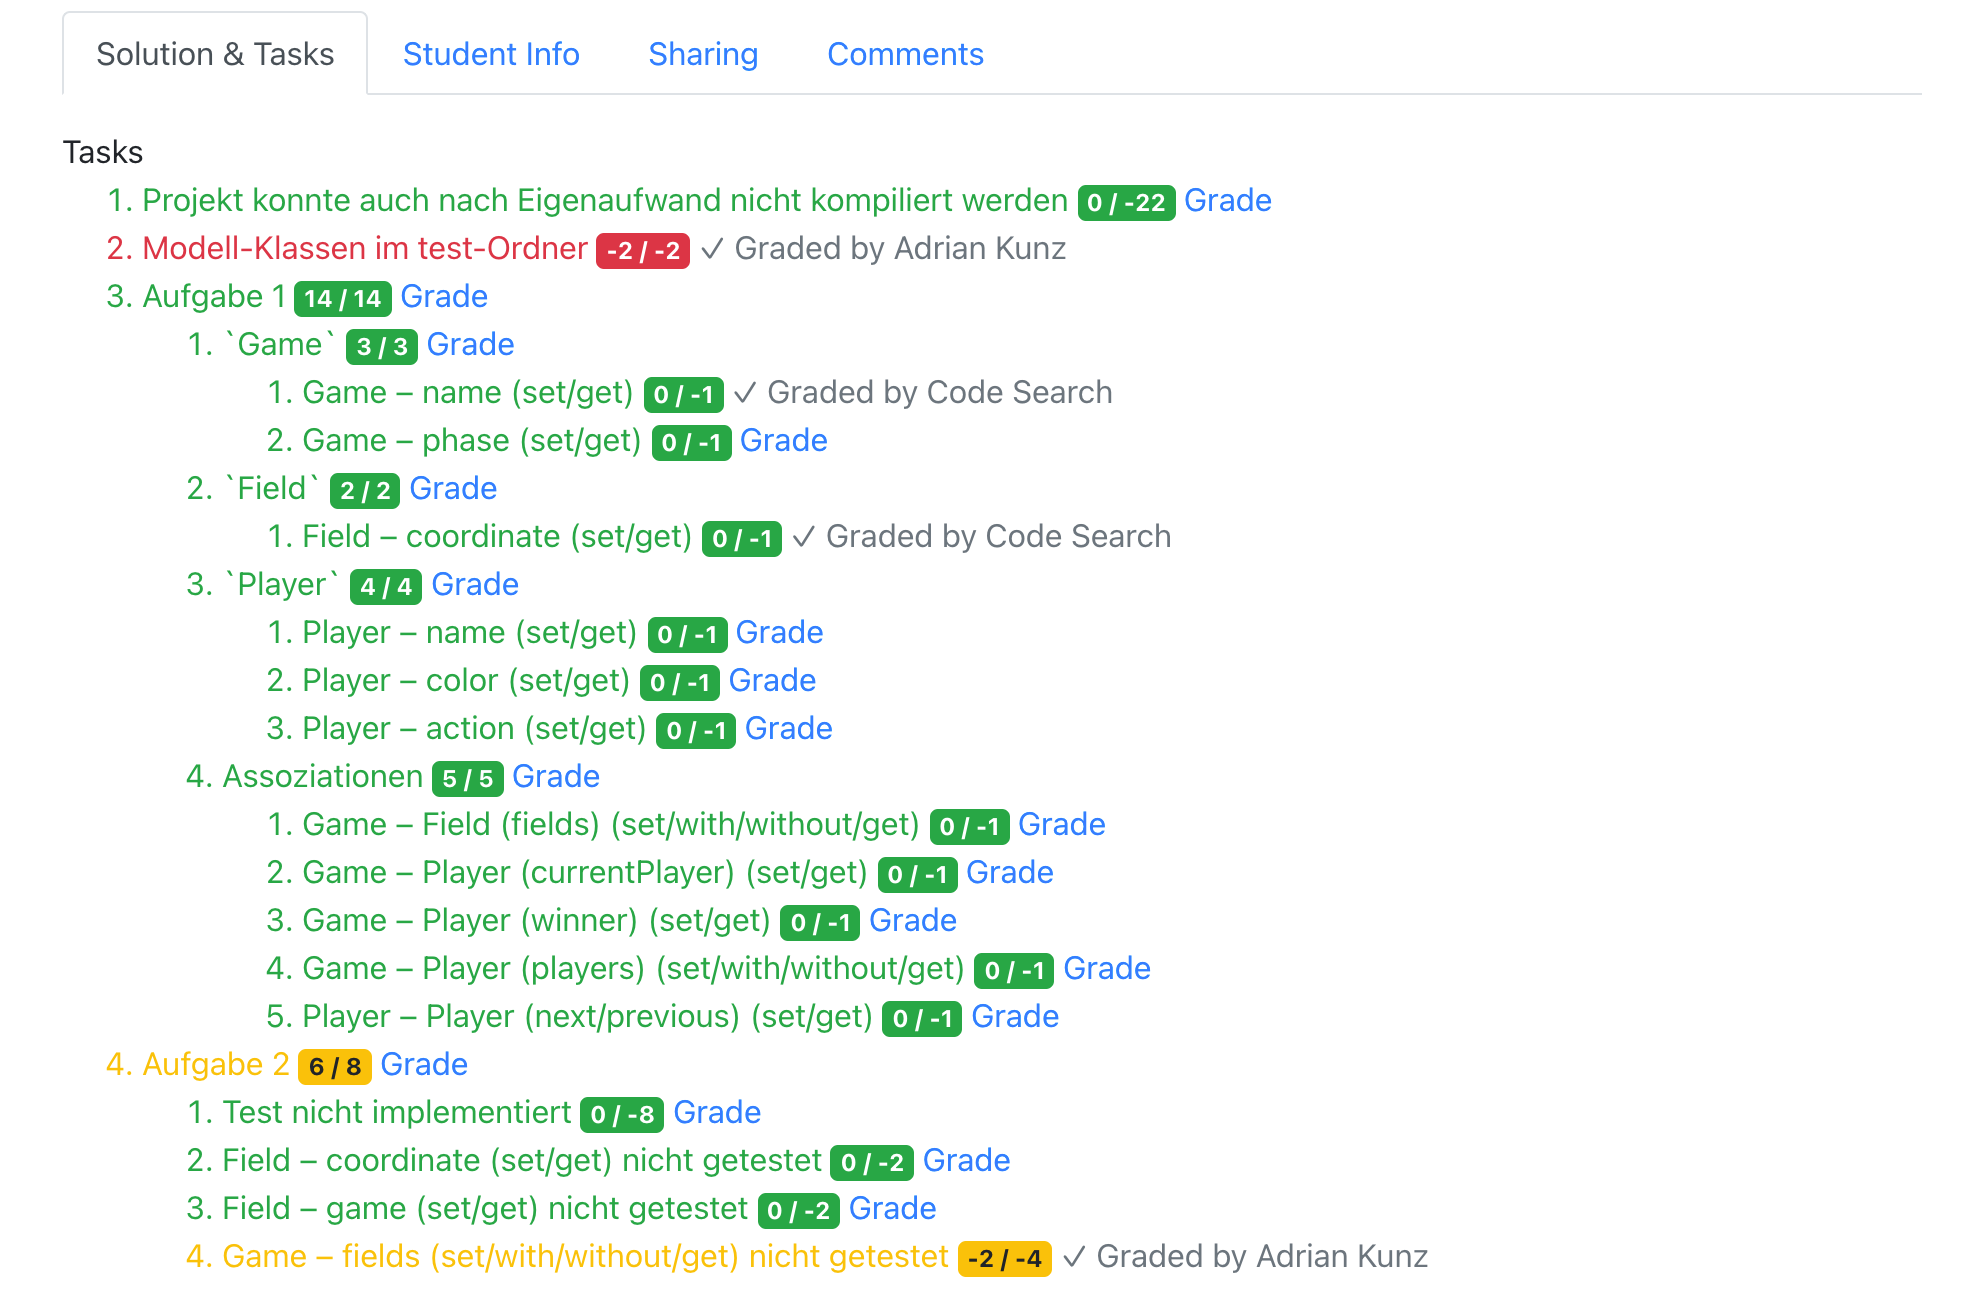
\includegraphics[width=\textwidth]{images/solution-tasks}
    \caption{Teilaufgaben in der Abgabe-Detailansicht}
    \label{fig:solution-tasks}
\end{figure}

Jede Teilaufgabe wird abhängig von der Punktzahl farblich markiert.
Entspricht die vergebene Punktzahl der Minimalpunktzahl eines Tasks, wird dieser rot (\ac{zB} -2/-2).
Werden die maximal mögliche Punkte erreicht, wird der Tasks grün (\ac{zB} 0/-1, 3/3).
Teilpunkte werden gelb dargestellt (\ac{zB} 6/8).
Dabei wird zwischen explizit vergebenen, berechneten und implizit vorhandenen Bewertungen unterschieden.
An der Bezeichnung \textbf{Graded by Name} statt \textbf{Grade} können von Bewertenden vergebene Punktzahlen identifiziert werden.
Teilaufgaben mit eigenen Unteraufgaben berechnen ihre Punktzahl durch Summieren der darunterliegenden Punkte\footnote{\todo{Stimmt nicht ganz, genau genommen Maximale Punktzahl - Summe der Maximalen Punktzahl positiver Unteraufgaben + Summe der Punktzahlen aller Unteraufgaben.}}.
Alle anderen Teilaufgaben erhalten standardmäßig null Punkte.
Durch Klicken auf \textbf{Grade} oder \textbf{Graded by Name} kann die Bewertung einer Teilaufgabe angelegt oder bearbeitet werden.
Abbildung~\ref{fig:evaluation-modal} das sich öffnende Modalfenster.

\begin{figure}
    \centering
    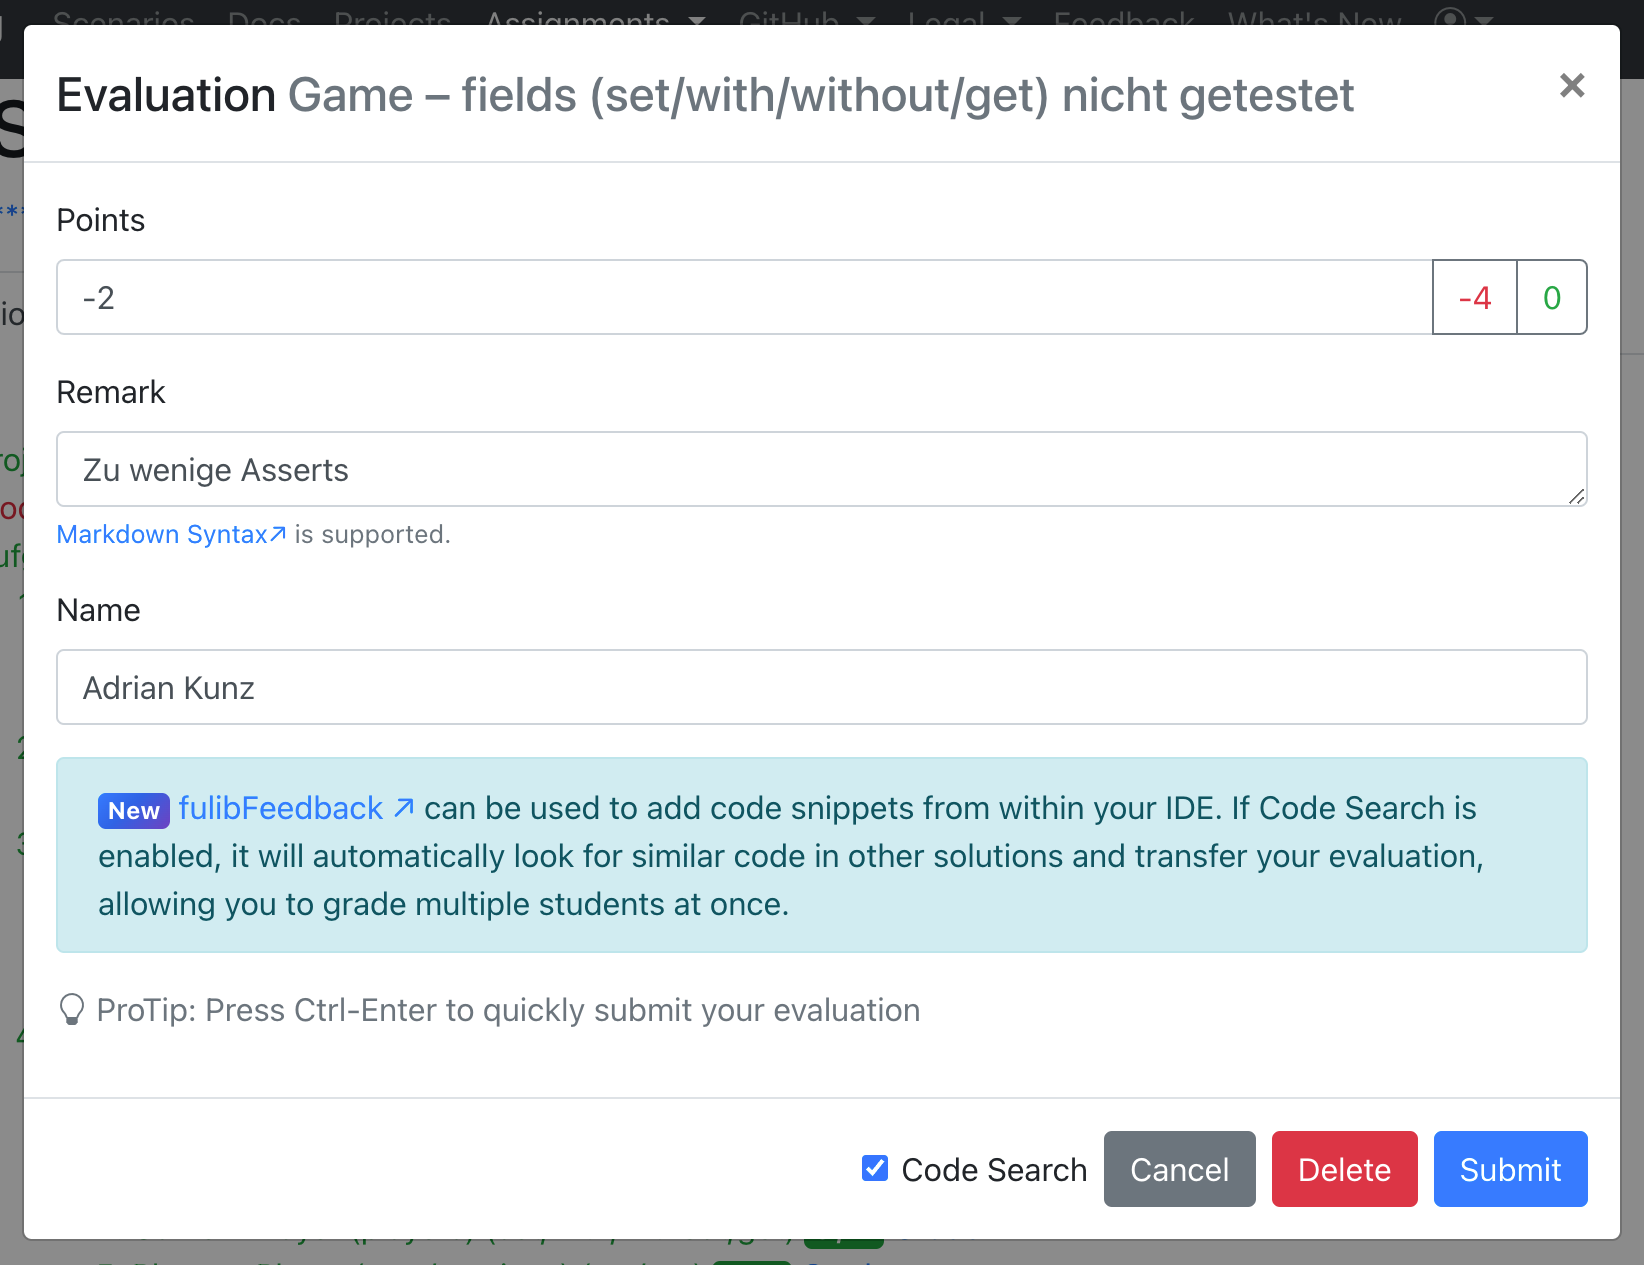
\includegraphics[width=0.8\textwidth]{images/evaluation-modal}
    \caption{Bewertung einer Teilaufgabe}
    \label{fig:evaluation-modal}
\end{figure}

Die Bewertung in dieser Fenster ist zunächst sehr einfach gehalten und für schnelle Bedienbarkeit optimiert.
Im ersten Eingabefeld kann die Punktzahl eingegeben werden oder durch die Kürzelbuttons direkt auf den Minimal- oder Maximalwert gesetzt werden.
Das Feld \textbf{Remark} kann für zusätzliche Hinweise für das Feedback verwendet werden.
Hier kann beispielsweise ein kurzer erklärender Satz oder nach dem Aufklappen zu einem mehrzeiligen Textbereich eine Fehlermeldung eingegeben werden.
Der \textbf{Name} dient der Identifikation des Bewerters, wird aber bei eingeloggten Benutzern oder vorheriger Eingabe automatisch ausgefüllt.
Der Informationstext zu fulibFeedback informiert über dessen Verfügbarkeit zum Hinterlegen von Codebeispielen.
Dies wird in Abschnitt~\ref{sec:fulibFeedback} erneut aufgefasst.
Mit dem \textbf{Submit}-Button wird schließlich die Bewertung gespeichert und das Modalfenster geschlossen.
In Abbildung~\ref{fig:evaluation-modal} wurde eine bereits vorhande Bewertung zum Bearbeiten geöffnet, weshalb der \textbf{Delete}-Button sichtbar ist, um diese zu löschen.

Die Bewertung von Teilaufgaben mit diesem Vorgehen ein wiederkehrender Ablauf, der von Bewertenden hunderte Male pro Hausaufgabe durchgeführt wird.
Daher wurde besonderer Wert darauf gelegt, den Ablauf möglichst effizient zu gestalten.
Während der Bewertung einer Teilaufgabe im Modalfenster wird die Zeit gemessen, die dabei verstrichen ist.
Darauf basierend wird eine Statistik berechnet, welche in Abschnitt~\ref{subsec:statistics} gezeigt und in Kapitel~\ref{ch:evaluation} für einige Realbeispiele ausgewertet wird.

\subsubsection{Feedback}

Der letzte Schritt der Bewertung eines Studierenden ist das Versenden des Feedbacks.
In der Abgabentabelle kann über den zugehörigen Button das Feedback-Modalfenster geöffnet werden, das in Abbildung~\ref{fig:submit-feedback} zu sehen ist.

\begin{figure}
    \centering
    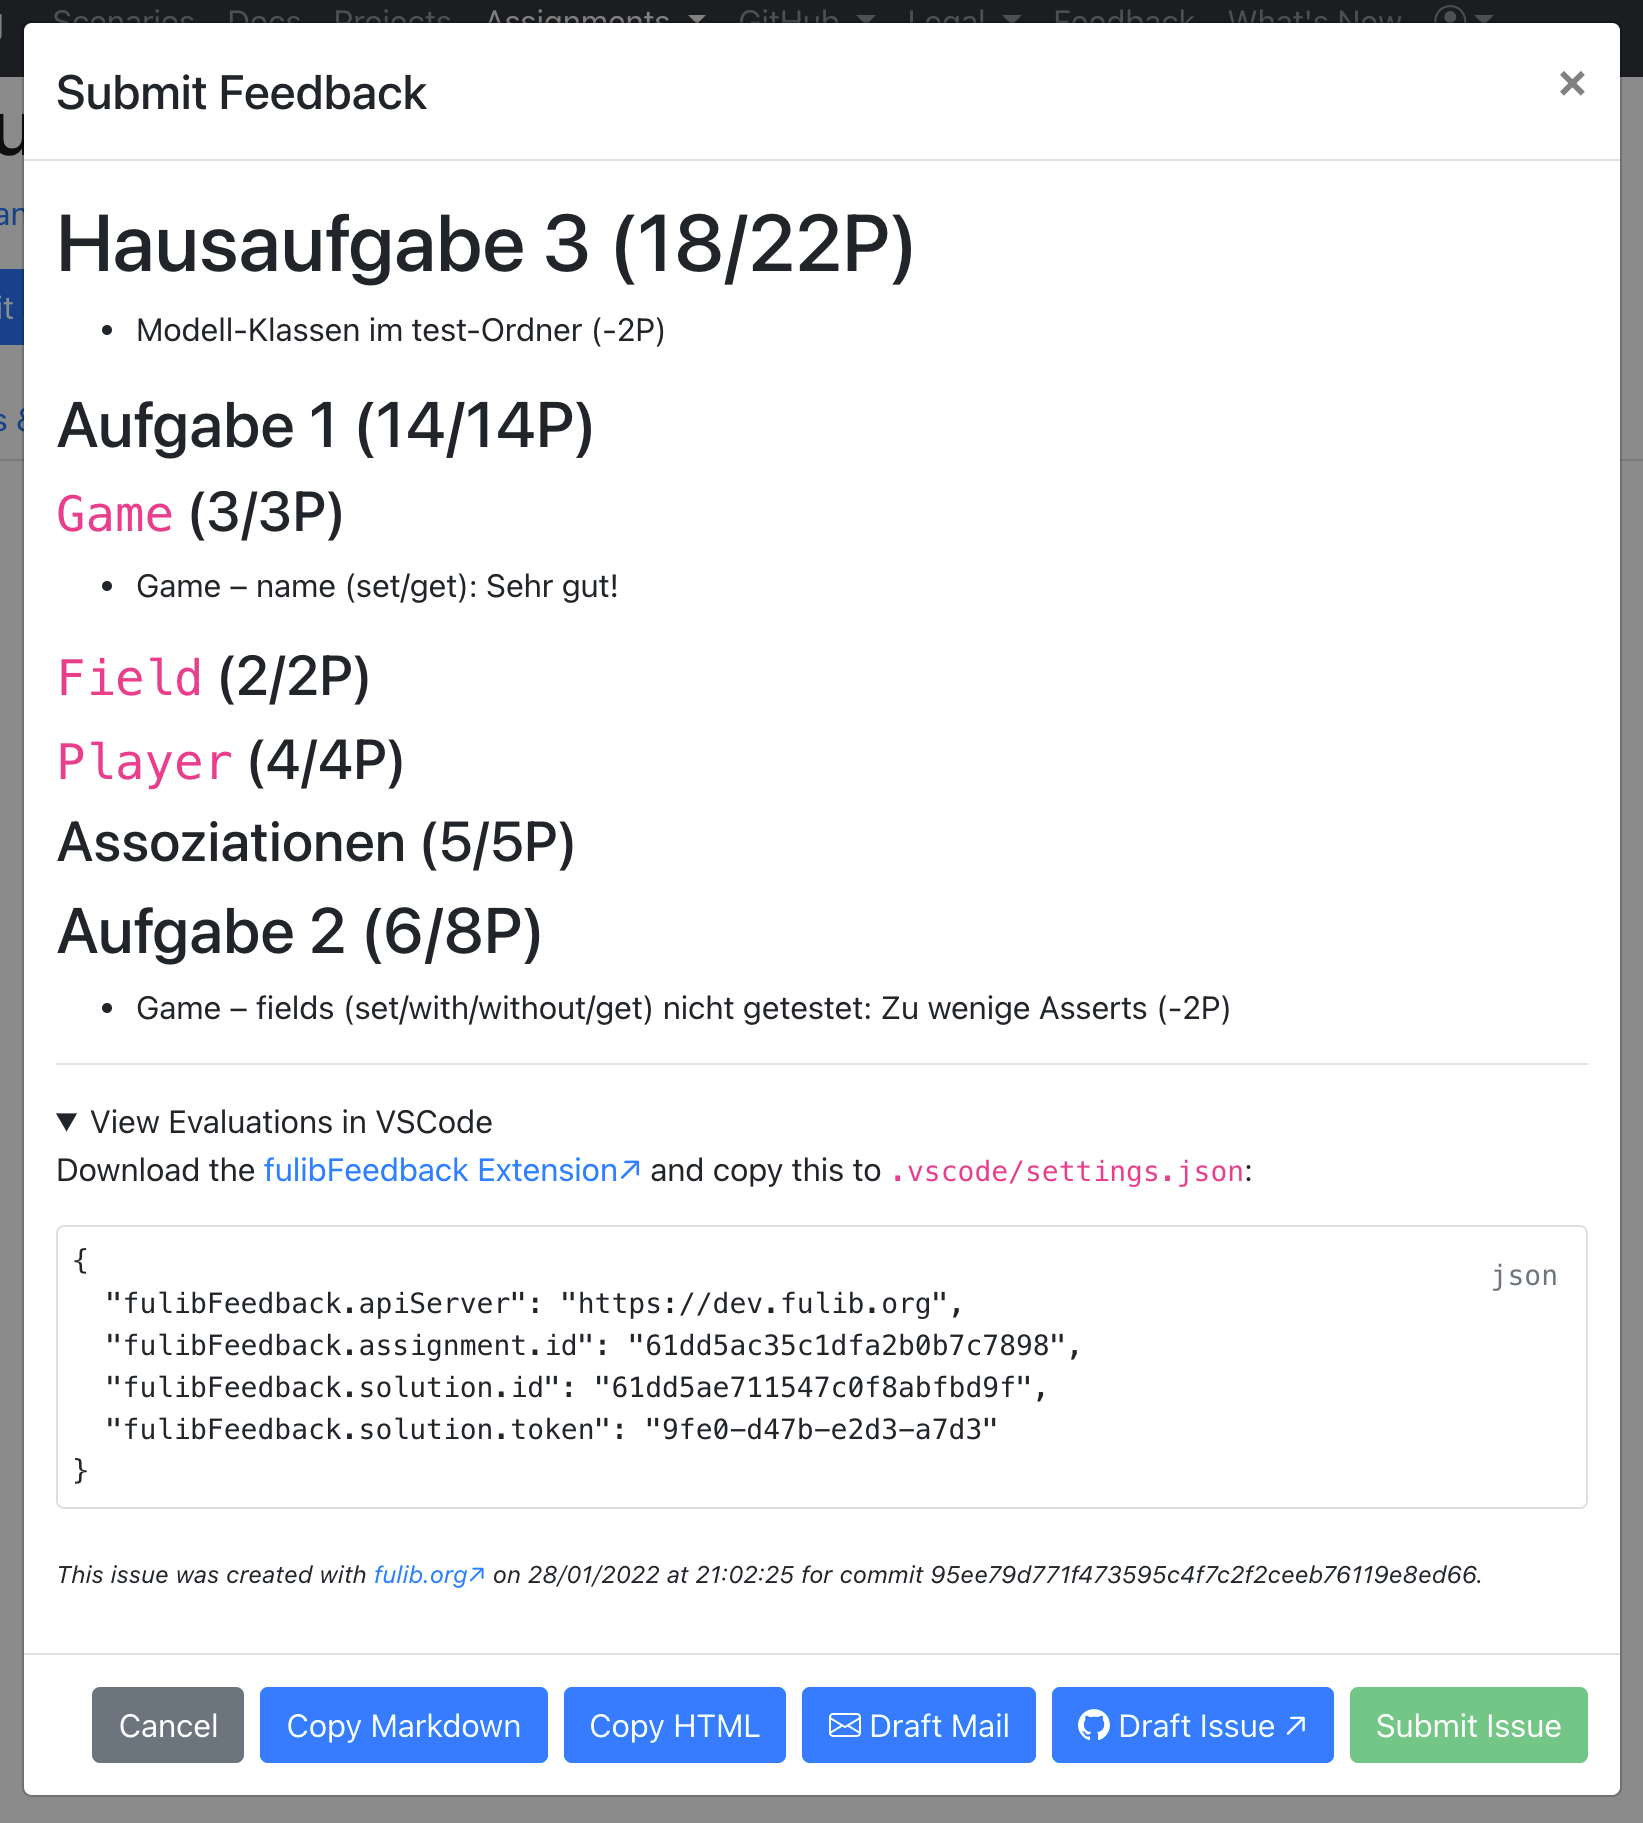
\includegraphics[width=0.8\textwidth]{images/submit-feedback}
    \caption{Modalfenster zum Versenden von Feedback}
    \label{fig:submit-feedback}
\end{figure}

Hier kann nochmal anhand der Vorschau abschließend geprüft werden, ob die Bewertung und Punkteberechnung korrekt durchgeführt wurde.
Daran können nun einige Aspekte der Feedback-Generierung erklärt werden.
Zunächst ist erkennbar, dass nicht jede Teilaufgabe des Assignments hier vertreten ist.
Insbesondere werden Abzüge, \ac{dh} Teilaufgaben mit negativer Punktzahl, nicht angezeigt, sofern sie nicht bewertet wurden.
In seltenen Fällen bietet es sich an, bei diesen Teilaufgaben keine Punkte abzuziehen, aber dennoch ein Kommentar oder eine Hilfestellung in Form des Remarks anzugeben.
Beispiel dafür ist die Teilaufgabe "Game -- name" in Abbildung~\ref{fig:submit-feedback}.
Die Punktzahl wird dann nicht angezeigt, da eine Darstellung wie "(0P)" zu Verwirrung führen könnte.
Teilaufgaben mit positiver Punktzahl werden immer angezeigt.

Am Ende der Bewertung befindet sich stets ein automatisch generierter Fußzeilenbereich.
Dort befinden sich Metadaten wie das Bewertungsdatum und der zugrundeliegende Commit.
Die fulibFeedback-Einstellungen für \ac{vsc} werden in Abschnitt~\ref{sec:fulibFeedback} erneut erwähnt.

Zum Versenden des Feedbacks werden mehrere Transportwege angeboten.
Mit den Buttons \textbf{Copy Markdown} und \textbf{Copy HTML} kann das Feedback im jeweiligen Textformat in die Zwischenablage kopiert werden.
\textbf{Draft Mail} öffnet das Standard-Mailprogramm des Benutzers und füllt automatisch den Rumpf der Email mit dem Feedback.
Soll die Bewertung über GitHub erfolgen, wie es in diesem Anwendungsbeispiel intendiert ist, gibt es zwei Möglichkeiten des Versands.
Einerseits kann das Formular zum Anlegen eines Issues auf GitHub mit \textbf{Draft Issue} geöffnet werden, sodass ein weiteres Mal der Text überprüft werden kann.
Andererseits kann mit \textbf{Submit Issue} direkt ein Issue über die GitHub \ac{api} und angelegt und somit ein Schritt gespart werden.
In jedem Fall wird die Gesamtpunktzahl, in Abbildung~\ref{fig:submit-feedback} beispielhaft 18/22, für die Abgabe gespeichert, damit sie in der Tabelle mit allen Abgaben angezeigt und die Abgabe eindeutig als bearbeitet erkannt werden kann.
Die Bewertung des Studierenden ist nun abgeschlossen und es kann mit der nächsten fortgefahren werden.

\subsection{Statistiken}\label{subsec:statistics}

Während und nach der Bewertung aller Abgaben können Betreuende und Übungsleitende eine Statistik einsehen.
Sie enthält Informationen über die Anzahl der Bewertungen, die dabei verstrichene Zeit und die Effektivität der automatischen Bewertung von Code Search.
Diese werden sowohl übergreifend als auch pro Teilaufgabe dargestellt.
Zusätzlich wird Einsicht darüber geboten, welche Teilaufgaben am häufigsten zu Punkteeinbußen oder -Abzügen geführt haben.
Daraus lässt sich ableiten, ob Lernziele möglicherweise nicht erreicht werden konnten oder Schwierigkeiten bei der Umsetzung bestanden.

Die Statistik kann in der Assignment-Übersicht unter dem gleichbenannten Tab gefunden werden.
In Abbildung~\ref{fig:assignment-statistics-basics} sind zunächst die übergreifenden Informationen dargestellt.
Die Seite gliedert sich in drei Abschnitte, \textbf{Solutions}, \textbf{Evaluations} und \textbf{Time Tracking}.

\begin{figure}
    \centering
    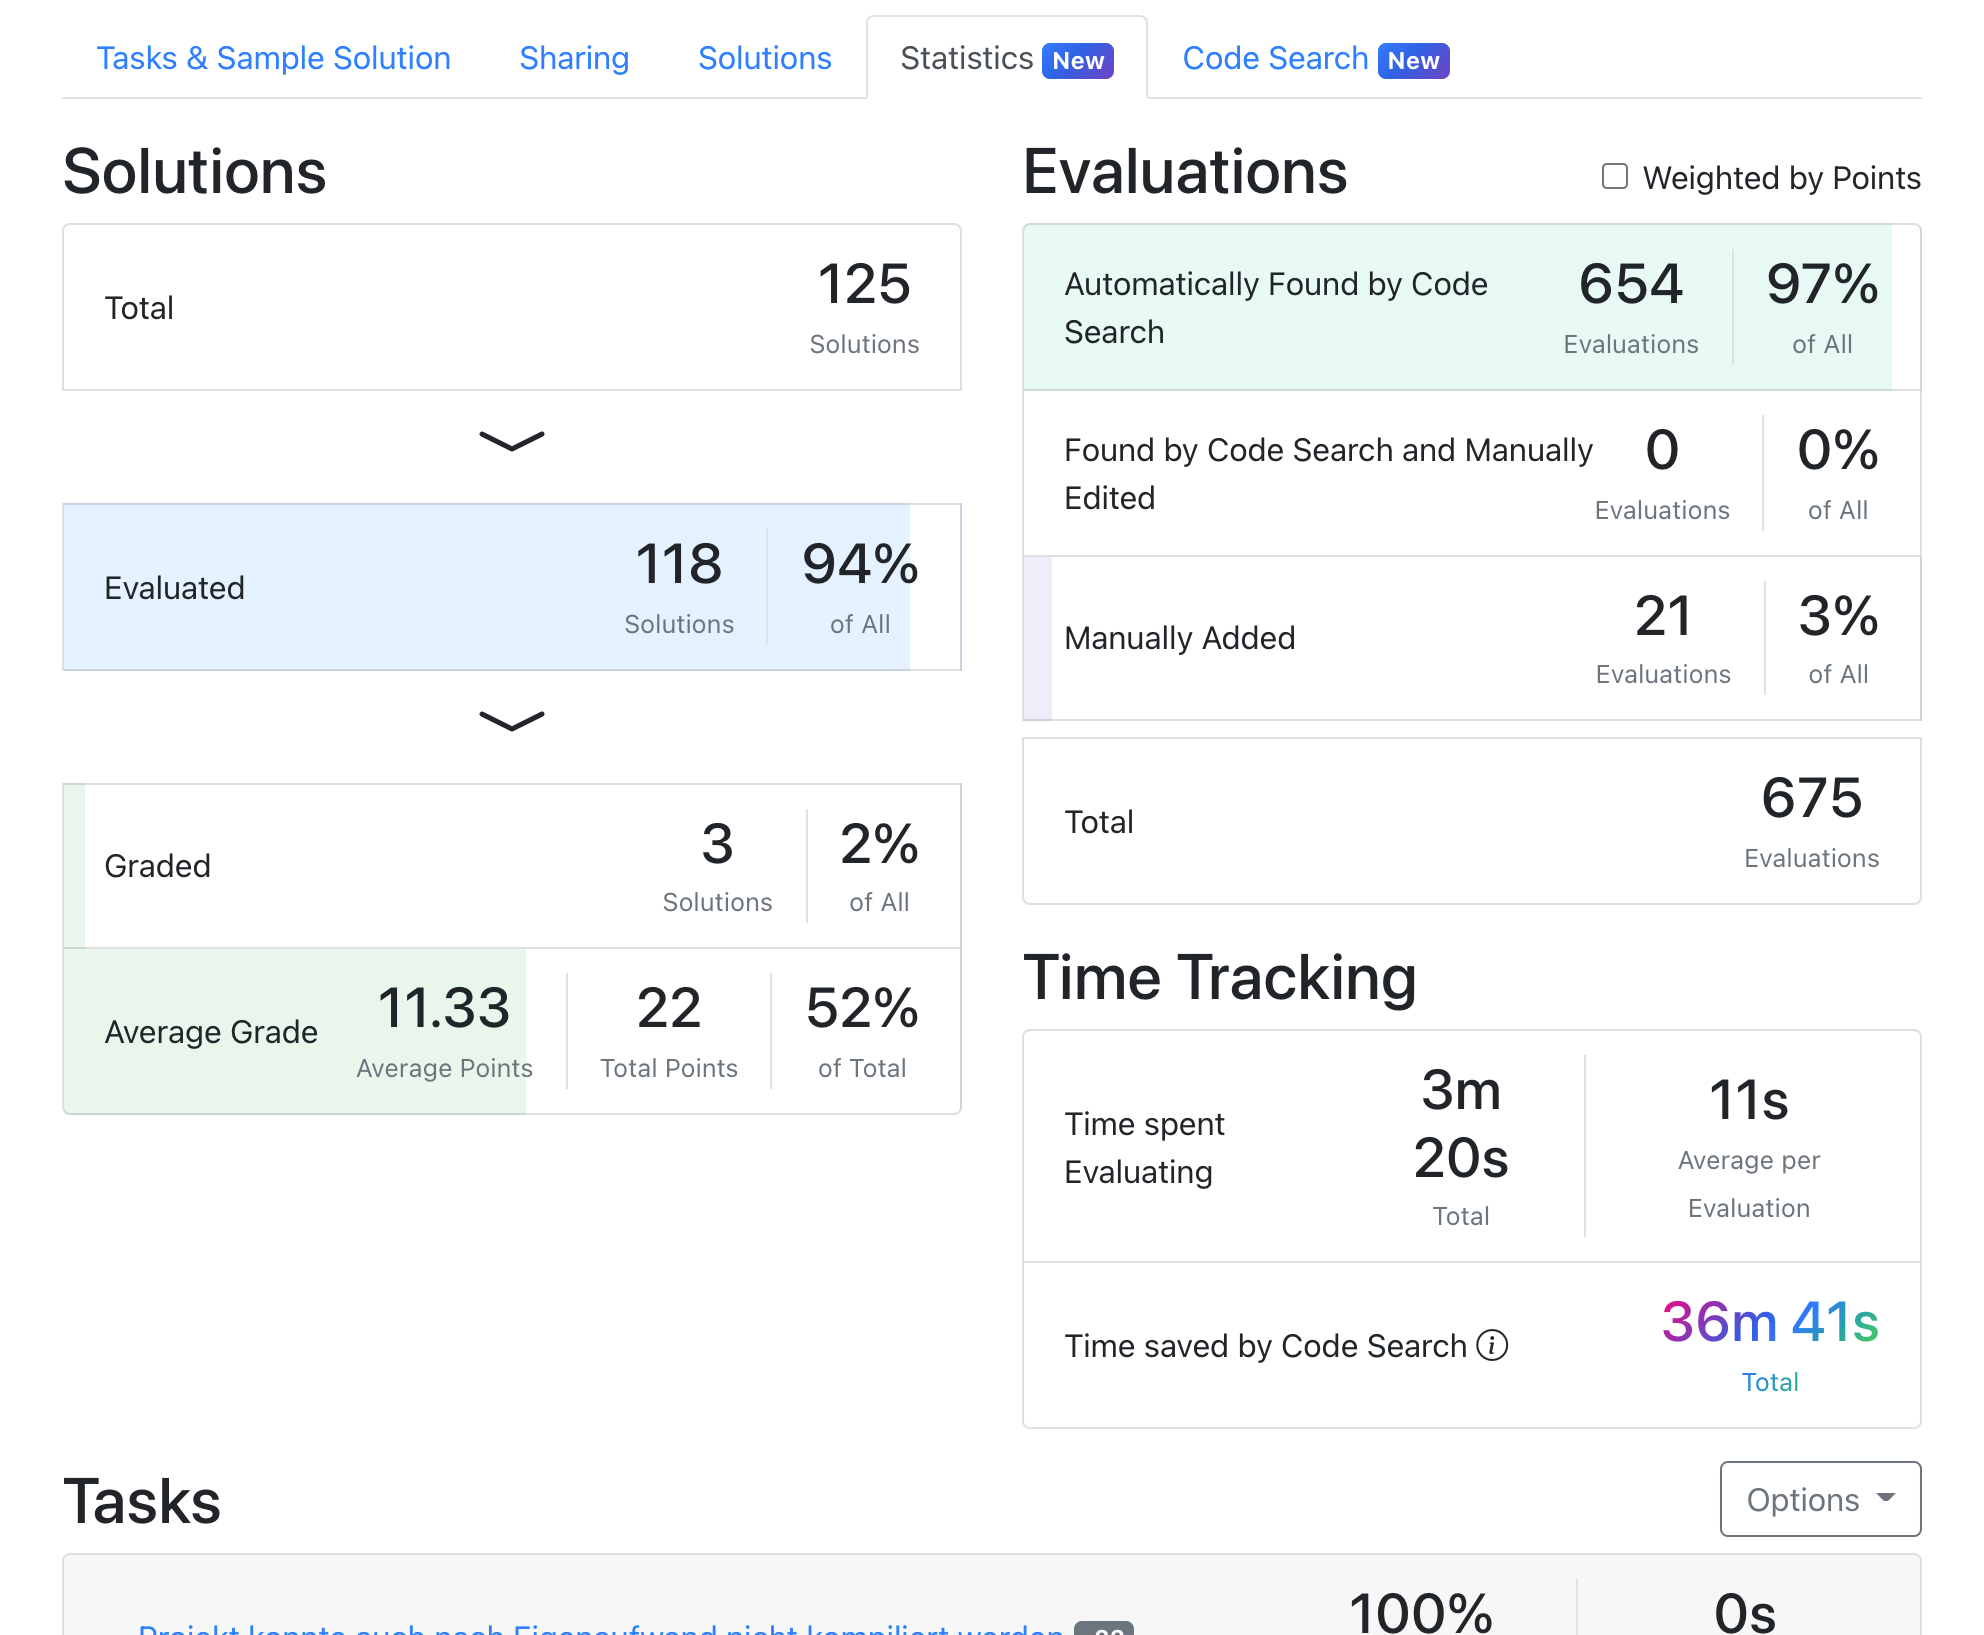
\includegraphics[width=\textwidth]{images/assignment-statistics-basics}
    \caption{Übergreifende Statistiken}
    \label{fig:assignment-statistics-basics}
\end{figure}

Unter Solutions ist jeweils die Anzahl der Abgaben insgesamt (\textbf{Total}), mit angefangener Bewertung (\textbf{Evaluated}) und mit versendeten Feedback abgeschlossenen (\textbf{Graded}) sichtbar.
Zudem wird die durchschnittlich erreichte Punktzahl der abgeschlossenen Abgaben abgezeigt\footnote{Es handelt sich bei diesem und folgenden Screenshots der Statistik nicht um die realen Zahlen der Hausaufgabe 3.}.

Die Evaluations\footnote{Bewertungen von Teilaufgaben.} werden für die Auswertung in drei Kategorien unterteilt.
Händisch hinzugefügte Bewertungen sind genau diejenigen, die wie in Abschnitt~\ref{subsec:grading} beschrieben erstellt wurden.
Von Code Search gefundene Bewertungen können anhand der vorherigen erstellt werden und geben Aufschluss darüber, wie effektiv das Werkzeug für die vorliegende Hausaufgabe war.
In seltenen Fällen ist es notwendig, diese automatisch erstellten Bewertungen händisch anzupassen, wenn beispielsweise eine Suche zu ungeeigneten Ergebnisse geführt hat.
Diese Fehlerfälle sowie die sich ergebenden relativen Anteile der Kategorien werden in Kapitel~\ref{ch:evaluation} näher erläutert und diskutiert.

Der Abschnitt Time Tracking dient der Berechnung der Effizienz von Bewertenden und Code Search.
Anhand der Zeitmessung, die während der Bewertung von Teilaufgaben stattfindet, können hier eine Gesamtdauer und der Durchschnitt pro Teilaufgabe berechnet werden.
Weiterhin wird hier angezeigt, wie viel Zeit durch die Verwendung von Code Search eingespart werden konnte.
Die Berechnung dieses Werts erfordert die Betrachtung der Teilaufgaben und wird in Kürze erläutert.
Kapitel~\ref{ch:evaluation} wird diesen Messwert anhand einiger realer Beispiele verwenden, um die Effizienz von Code Search zu bestimmen.

\begin{figure}
    \centering
    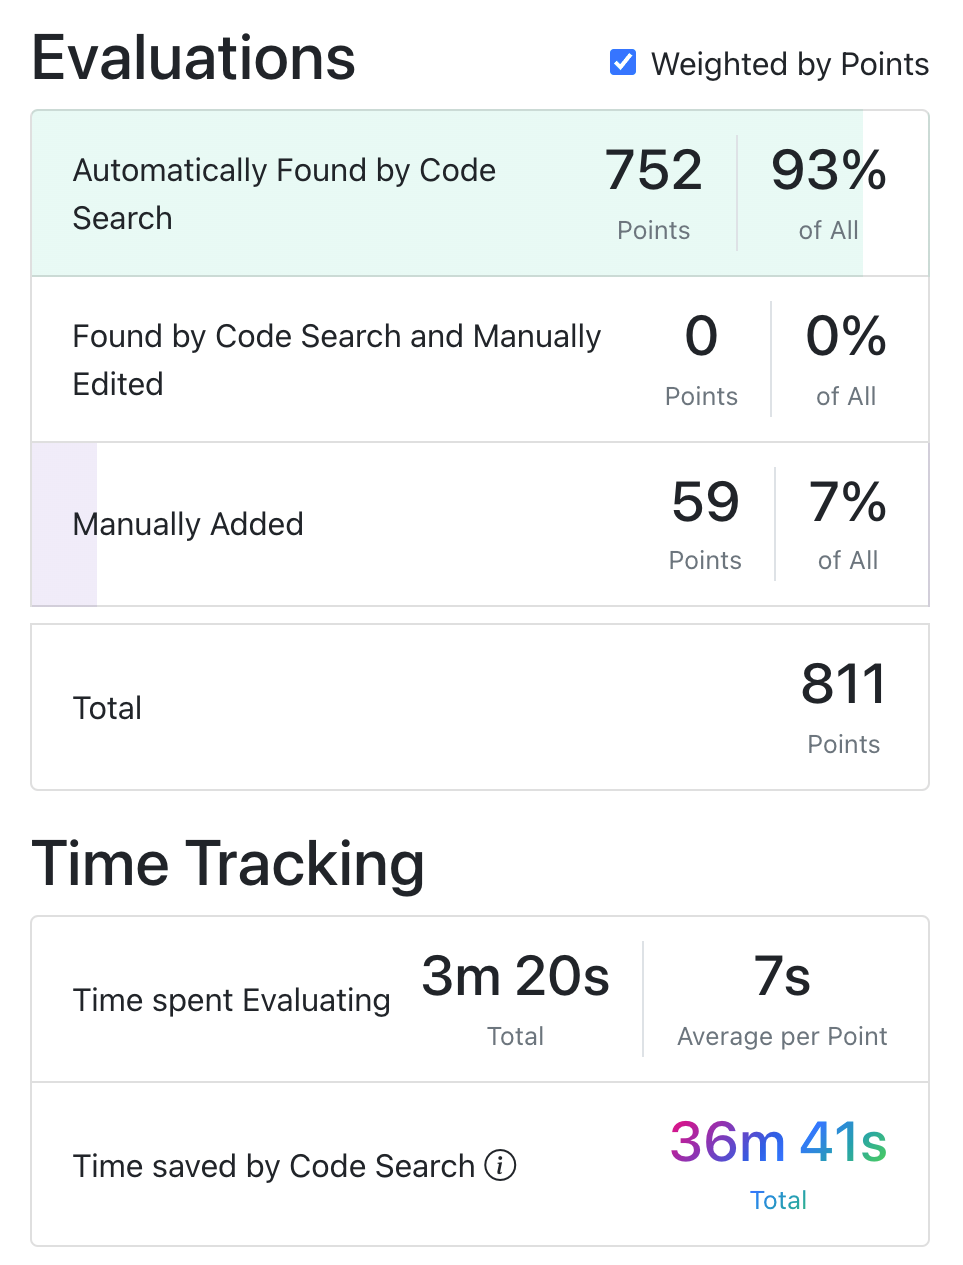
\includegraphics[width=0.5\textwidth]{images/assignment-statistics-by-points}
    \caption{Statistiken gewichtet nach Punkten}
    \label{fig:assignment-statistics-by-points}
\end{figure}

Evaluations und Time Tracking können die Ansicht verändern, um Punktzahlen statt Bewertungen von Teilaufgaben als Bewertungsgrundlage zu verwenden.
Dafür wird der Haken \textbf{Weighted by Points} gesetzt, wie Abbildung~\ref{fig:assignment-statistics-by-points} zeigt.
\todom{
    Wofür ist das eigentlich gut?
    Um Einschäten zu können, ob die Punkte mit dem Arbeitsaufwand bei der Bewertung übereinstimmen?
    Idealerweise gäbe es für jeden Punkt eine Teilaufgabe - siehe z.B. PM Blatt 8.
}

\begin{figure}
    \centering
    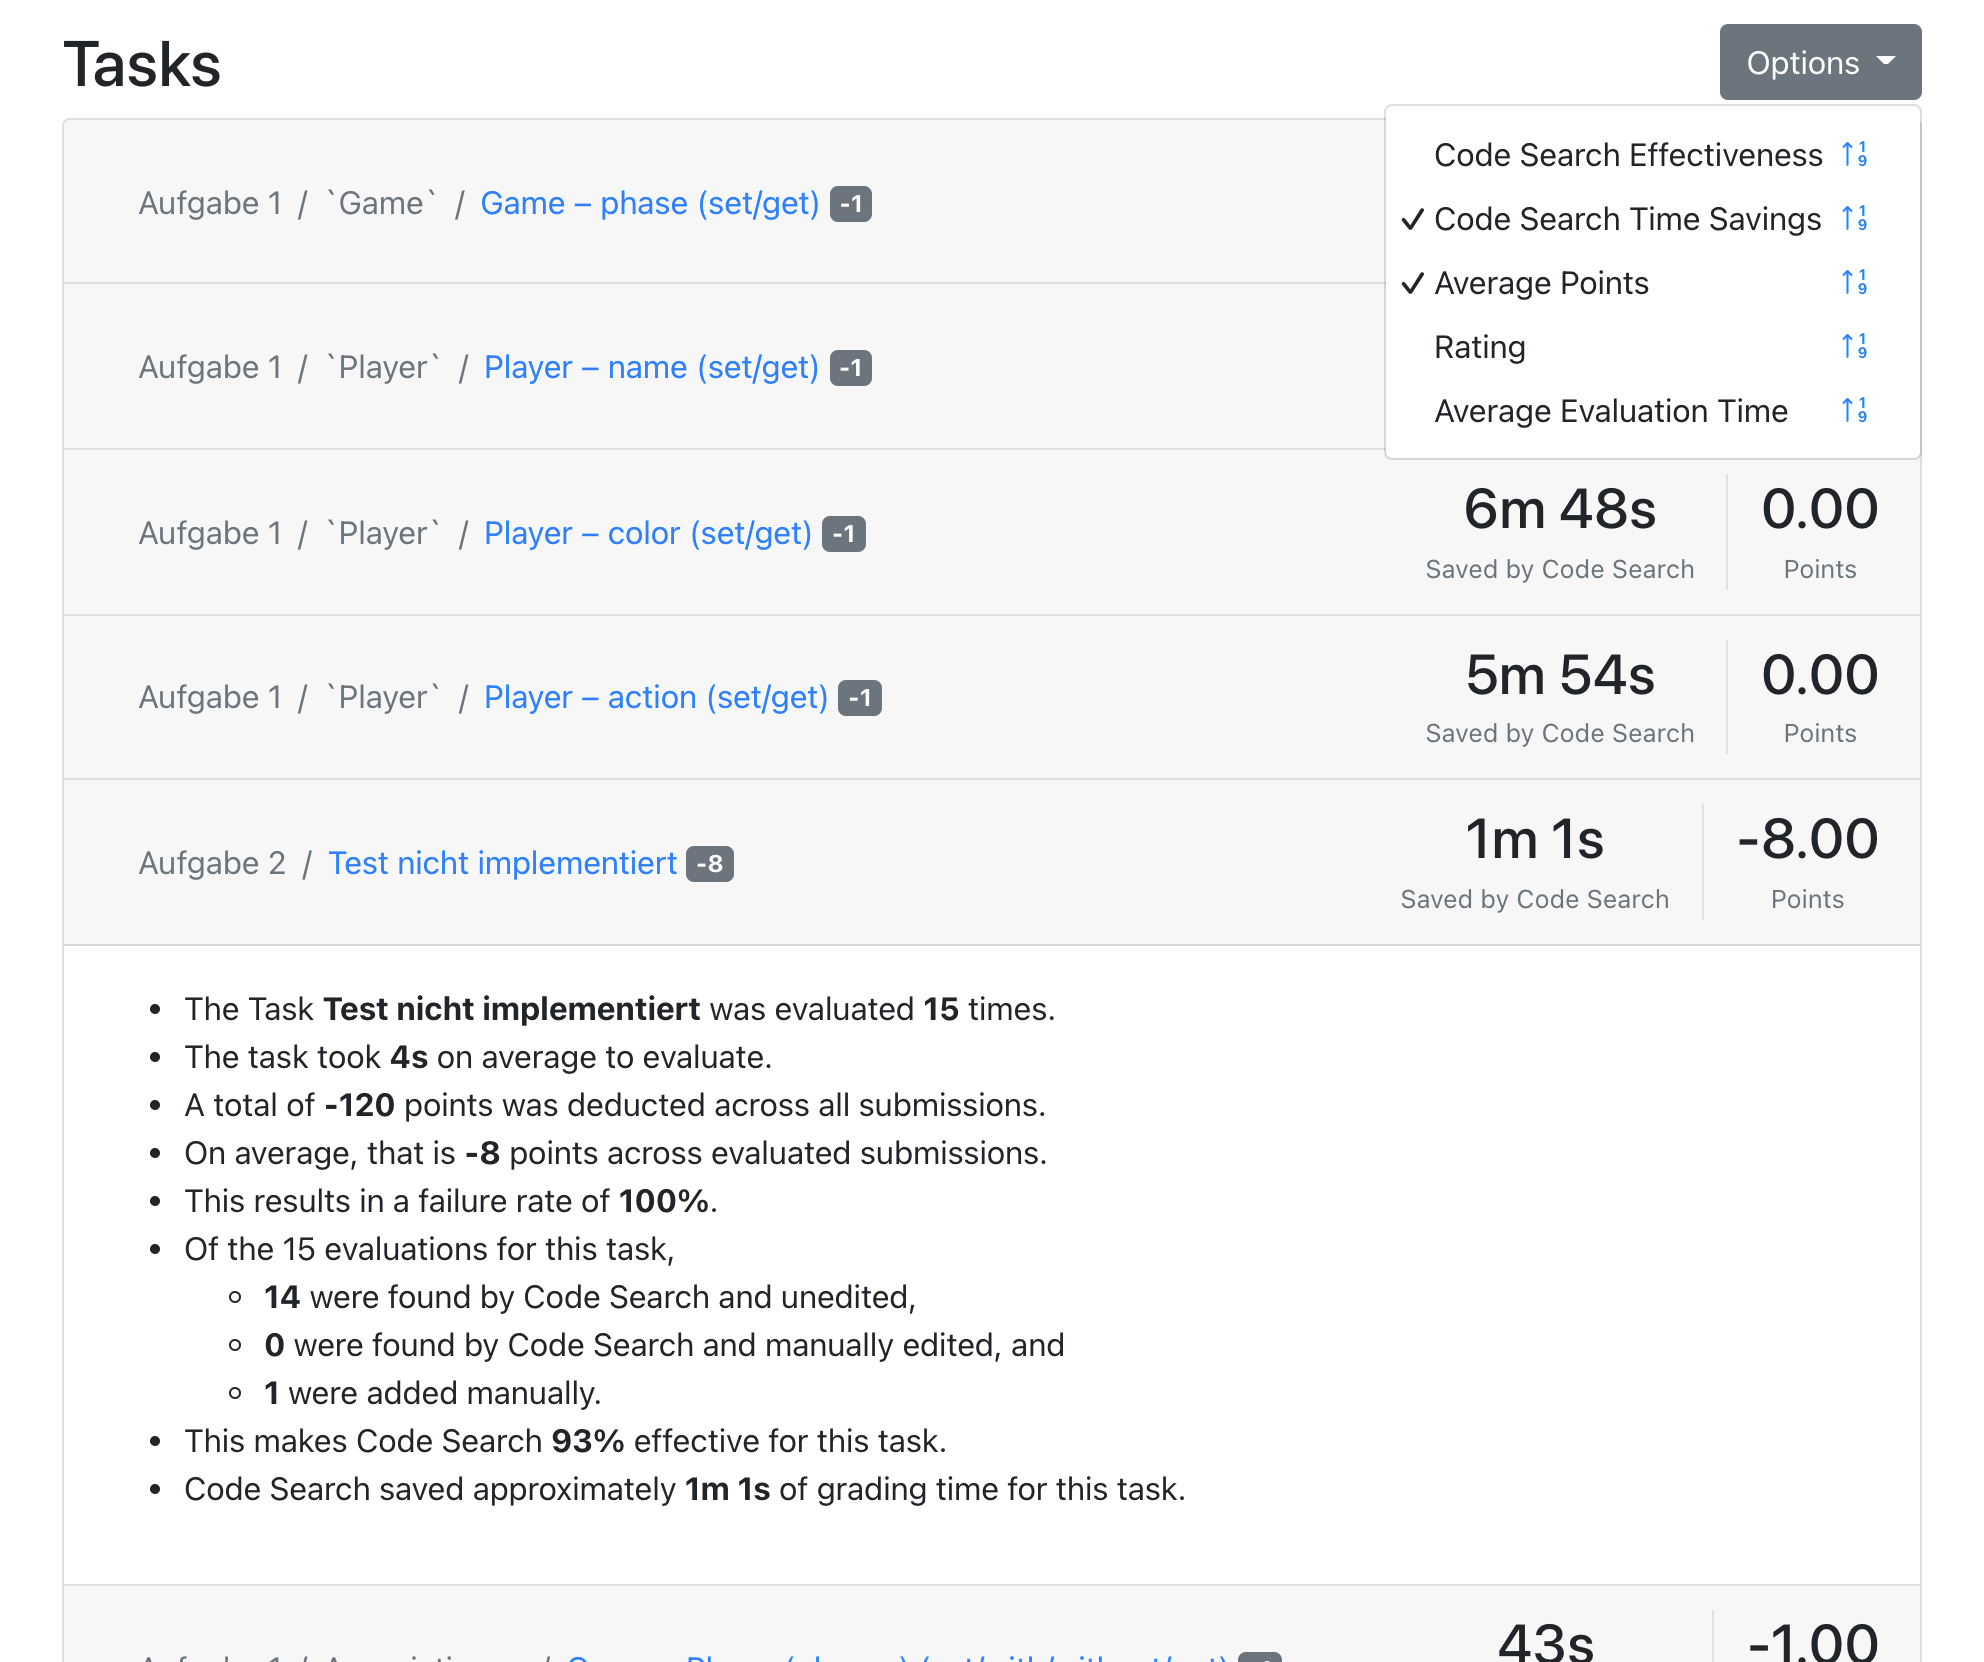
\includegraphics[width=\textwidth]{images/assignment-statistics-tasks.png}
    \caption{Statistiken für einzelne Teilaufgaben}
    \label{fig:assignment-statistics-tasks}
\end{figure}

Im unteren Teil der Statistik befindet sich eine Liste aller Teilaufgaben, wie Abbildung~\ref{fig:assignment-statistics-tasks} zeigt.
Die Informationen in der Kopfzeile jedes Eintrags sind mit dem Options-Menü auswählbar.
Dort kann zwischen den wichtigsten Metriken ausgewählt werden.
Diese werden nachfolgend kurz beschrieben.
Zudem kann die Liste anhand der Werte auf- oder absteigend sortiert werden.
Jeder Eintrag kann individuell ausgeklappt werden, um weitere Details anzuzeigen.
Dafür werden jeweils kurze Stichpunkte zu jedem Wert genannt, um Hinweise auf dessen Bedeutung zu geben.

\begin{description}
    \item[Code Search Effektiveness] ist der Anteil der Bewertungen für diese Teilaufgabe, die automatisch von Code Search angelegt wurden.
    Im Beispiel der Teilaufgabe \textbf{Aufgabe 2 / Test nicht implementiert} wurde eine Bewertung händisch angelegt und darauf basierend 14 von Code Search erstellt.
    Dies ergibt eine Effektivität von $\frac{14}{1 + 14} = \frac{14}{15} \approx 93\%$.
    \footnote{Die Effektivität kann nie 100\% betragen, da Code Search nur ausgehend von einer händischen Bewertung aktiviert wird. Beim Löschen von dieser werden auch davon abstammende Code Search-Bewertungen gelöscht.}
    \item[Average Evaluation Item] ist die durchschnittliche Bewertungsdauer der Teilaufgabe.
    Diese wird gemessen, während das Bewertungs-Modalfenster geöffnet ist.
    Um zu vermeiden, dass das verlängerte Öffnen dieses Fensters, beispielsweise beim Verlassen des Arbeitsplatzes oder beim einlegen einer Pause, die Statistik verfälscht, werden hier Ausreißer länger als 60 Sekunden nicht im Durchschnitt verrechnet.
    \item[Code Search Time Savings] bezeichnet die geschätze Zeit, die durch Code Search bei der Bewertung dieser Teilaufgabe eingespart wurde.
    Sie berechnet sich durch Multiplikation der Average Evaluation Time mit der Anzahl der von Code Search erstellten Bewertungen.
    Die Summe dieser Werte über alle Teilaufgaben ergibt die zuvor genannte Zeit, die insgesamt mit Code Search gespart wurde.
    \item[Average Points] ist die durchschnittlich vergebene Punktzahl über alle Bewertungen dieser Teilaufgabe.
    \item[Rating] ergibt sich aus den Average Points geteilt durch die maximal erreichbare Punktzahl der Teilaufgabe.
    Dadurch ergibt sich eine relative Prozentangabe, die mit anderen Teilaufgaben verglichen werden kann.
    Mit diesem Wert können insbesondere die Teilaufgaben identifiziert werden, die am häufigsten zu Punktabzug geführt haben und mögliche Problemquellen für Studierende darstellen.
\end{description}

\subsection{Code Search}\label{subsec:code-search}

\todo{
    Code Search als Anwendung von Elasticsearch.
}

\section{fulibFeedback}\label{sec:fulibFeedback}

\subsection{VSCode Extension}\label{subsec:vscode-extension}

\todo{
    Einfacher Client für Language Server.
    Einstellungen.
    Protocol Handler für Konfiguration.
}

\subsection{Language Server}\label{subsec:language-server}

\todo{
    Selection und Diagnostics.
    Wiederverwendbar für andere IDEs.
}

    \chapter{Evaluation}\label{ch:evaluation}

Die in Kapitel~\ref{ch:implementation} entstandene Software wurde im Verlauf dieser Arbeit einer umfangreichen Evaluierungsphase unterzogen.
Dadurch konnten individuelle Abläufe ermöglicht, unvorhergesehene Benutzerinteraktionen erfasst und ergonomische Bedienbarkeit sichergestellt werden.
In diesem Kapitel werden drei Anwendungsfälle betrachtet, in denen die Werkzeuge fulib.org und fulibFeedback verwendet wurden.
Dabei handelt es sich um drei Veranstaltungen der Universität Kassel aus dem Sommer- bis Wintersemester 2021 bis 2022.
In Abschnitt~\ref{sec:pm-2021-2022} wird zunächst die Veranstaltung \ac{pm}\footnote{
    Fachgebiet Softwaretechnik, Prof.\ Dr.\ Albert Zündorf.
} des Wintersemesters 2021/22 betrachtet.
Die Abschnitte~\ref{sec:algods-2021} und~\ref{sec:einfinf-2021-2022} bieten daraufhin Einblicke in die Veranstaltungen "Algorithmen und Datenstrukturen"\footnote{
    Fachgebiet Programmiersprachen/-Methodik, Prof.\ Dr.\ Claudia Fohry.\label{fn:fg-plm}
} im Sommersemester 2021 und "Einführung in die Informatik"\footref{fn:fg-plm} im Wintersemester 2021/22.

\section{\acl{pm}}\label{sec:pm-2021-2022}

Die Veranstaltung \ac{pm} stellt die größten Teil der Evaluation dar.
Sie umfasste insgesamt elf Aufgabenblätter und ein Abschlussprojekt, welche von bis zu 125 Studierenden bearbeitet und bis zu sechs Personen mit fulib.org und fulibFeedback bewertet wurden.

Im Verlauf der Veranstaltung wurde die Anzahl der Benutzer stets erhöht, um anfangs mögliche Probleme zu ermitteln und dabei zu vermeiden, dass viele Personen davon betroffen und verlangsamt werden.
Jeder neue Benutzer erhielt eine kurze Einweisung in die Bedienung der Werkzeuge und Hinweise zur optimalen Verwendung.

Während der Bewertung sind individuelle Anmerkungen sowie eine große Anzahl von Metriken durch die Statistiken auf fulib.org entstanden.
In diesem Abschnitt werden einige Ansichten der Benutzer erläutert (Abschnitt~\ref{subsec:user-feedback}) und die Rohdaten der Statistiken erfasst (Abschnitt~\ref{subsec:pm-metrics}).
Des Weiteren wird erläutert, welche Erfahrung mit den Werkzeugen zu Anpassungen der Aufgabenstellungen und Bewertungskriterien geführt haben, um den Ablauf der Bewertung zu optimieren (Abschnitt~\ref{subsec:pm-adaptations}).
Da sich die Beobachtungen und Metriken stets auf einzelne Übungsblätter beziehen, ist es an dieser Stelle lohnenswert, die elf \acp{ha} kurz zu beschreiben.

\begin{description}
    \item[\ac{ha}1] führt die Versionskontrolle mit Git ein, festigt den Unterschied zwischen den Konzepten "Abstrakt" und "Konkret" und führt Szenarien ein.\footnote{
        \url{https://seblog.cs.uni-kassel.de/wp-content/uploads/2021/10/PMWS2122_HA1.pdf}
    }
    \item[\ac{ha}2] beschäftigt sich mit Objekt- und Klassendiagrammen, die aus gegebenen Szenarien abgeleitet werden sollen.\footnote{
        \url{https://seblog.cs.uni-kassel.de/wp-content/uploads/2021/11/PMWS2122_HA2.pdf}
    }
    \item[\ac{ha}3] erwartet die händische Implementierung eines Datenmodells mit besonderem Augenmerk auf die korrekte Sicherstellung von referentieller Integrität.
    Einige prüfende Tests sind vorgegeben, ein weiterer muss selbst implementiert werden.\footnote{
        \url{https://seblog.cs.uni-kassel.de/wp-content/uploads/2021/11/PM2022_Hausaufgabe03.pdf}
    }
    \item[\ac{ha}4] führt fulib als Werkzeug zur Datenmodell-Generierung ein und ersetzt damit die händische Implementierung von \ac{ha}3.
    Darauf aufbauend soll erste Logik zur Initialisierung eines Spiels implementiert und getestet werden.\footnote{
        \url{https://seblog.cs.uni-kassel.de/wp-content/uploads/2021/11/PM_2122_Hausaufgabe04.pdf}
    }
    \item[\ac{ha}5] übt Design und Planung von Benutzeroberflächen in Form von Wireframes.
    Davon unabhängig wird das Test-First-Prinzip anhand von weiterer Spiellogik erprobt.\footnote{
        \url{https://seblog.cs.uni-kassel.de/wp-content/uploads/2021/12/PM_2022_Hausaufgabe05.pdf}
    }
    \item[\ac{ha}6] erwartet, dass die zuvor erstellten Oberflächendesigns mit \acp{fxml}\footnote{
        \ac{xml}-ähnliche Beschreibung von Oberflächen für das JavaFX-Framework.
    } umgesetzt und mit JavaFX zu einer ausführbaren Anwendung gemacht werden.
    Deren Oberfläche soll mit der TestFX-Bibliothek getestet werden.\footnote{
        \url{https://seblog.cs.uni-kassel.de/wp-content/uploads/2021/12/PM_2021_Hausaufgabe06.pdf}
    }
    \item[\ac{ha}7] beinhaltet die weitere Implementierung von Spiellogik, die dynamische Umsetzung der Oberfläche mit Controllern und zugehörige Tests.\footnote{
        \url{https://seblog.cs.uni-kassel.de/wp-content/uploads/2022/01/PM_2022_Hausaufgabe07.pdf}
    }
    \item[\ac{ha}8] verknüpft Modell und Oberfläche und hält diese bei jeder Änderung synchron, implementiert die verbleibende Spiellogik und testet den kritischen Pfad des fertigen Spiels.\footnote{
        \url{https://seblog.cs.uni-kassel.de/wp-content/uploads/2022/01/PM_2022_Hausaufgabe08.pdf}
    }
    \item[\ac{ha}9] beginnt ein neues Projekt, das initialisiert und mit einer einfachen Oberfläche versehen werden soll.\footnote{
        \url{https://seblog.cs.uni-kassel.de/wp-content/uploads/2022/01/PM_2022_Hausaufgabe09.pdf}
    }
    \item[\ac{ha}10] erweitert das neue Projekt um Serveranbindung mit \ac{rest} und dynamische Änderung der Oberfläche, um einen einfachen Chat zu ermöglichen.\footnote{
        \url{https://seblog.cs.uni-kassel.de/wp-content/uploads/2022/02/PM_WS2122_Hausaufgabe10.pdf}
    }
    \item[\ac{ha}11] ersetzt die \ac{rest}-Anbindung der vorherigen Hausaufgabe mit einer WebSocket-Schnittstelle.
    Darüber hinaus wird einfache Speicherung von Einstellungen mit \ac{json}-Dateien eingeführt.\footnote{
        \url{https://seblog.cs.uni-kassel.de/wp-content/uploads/2022/02/PM_2122_Hausaufgabe11.pdf}
    }
\end{description}

\subsection{Benutzer-Anmerkungen}\label{subsec:user-feedback}

Während der Testphase der Werkzeuge in \ac{pm} wurden die Bewertenden gebeten, nach jeder Hausaufgabe eine kurze Rückmeldung zu geben.
Diese konnte generelle Bemerkungen, Anfragen für neue Features, Verbesserungsvorschläge und kurze Fehlerberichte beinhalten.
Alle Rückmeldungen wurden in einem öffentlichen Issue\footnote{
    \url{https://github.com/fujaba/fulib.org/issues/196}
} auf GitHub gesammelt.
Nachfolgend werden einige der wichtigsten Erkenntnisse daraus beschrieben, da sie maßgeblich zu der Entwicklung von fulib.org und fulibFeedback beigetragen haben.

\subsubsection{Auswahl von Codeabschnitten}

Die wichtigste Erkenntnis aus den Benutzeranmerkungen war die Art und Weise, wie Codeabschnitte ausgewählt werden.
Der Ablauf, der in Abschnitt~\ref{subsec:choosing-code-snippets} beschrieben wurde und beide Werkzeuge symbiotisch kombiniert, wurde erst in einer späteren Version von fulibFeedback eingeführt.
Zuvor wurde die gesamte Bewertung von Code allein mit fulibFeedback gemacht.
Mittels Code Actions des \ac{lsp} wurde ein Menü angezeigt, das alle Teilaufgaben baumförmig anzeigte.
Die Aktivierung eines Menüeintrags hat dazu geführt, das über dem ausgewählten Quellcode ein Kommentar eingefügt wurde, in dem Punktzahl und Remark eingegeben werden konnten.
In diesem Kommentar konnten zwei Code Actions verwendet werden, um die Bewertung zu erstellen.
Diese Vorgehensweise hatte einige erheblich Nachteile:

\begin{itemize}
    \item Das Menü, das die Teilaufgaben anzeigte, konnte bei einer großen Anzahl von Teilaufgaben unübersichtlich werden und teilweise die Bildschirmhöhe überschreiten.
    Dies hat insbesondere die Effizienz eingeschränkt, da einige Zeit zum Suchen der nächsten unbewerteten Teilaufgabe notwendig war.
    \item Der automatisch erstellte Kommentar enthielt nur die \ac{id} der zuvor ausgewählten Teilaufgaben, aber nicht deren Beschreibung.
    Es kam vor, dass Bewertende versehentlich die falsche Teilaufgabe auswählten und dies nicht bemerkten, bevor die Bewertung erstellt wurde.
    \item Generell erforderte der automatisch erstellte Kommentar einen erheblichen Programmieraufwand seitens des Language Servers.
    Dies ist der Einschränkung des \ac{lsp} verschuldet, keine Möglichkeit zu bieten, als Teil einer Code Action den Benutzer des Editors nach einer Eingabe zu Frage.
    Wäre dies möglich, hätten Remark und Punktzahl beispielsweise über ein Prompt-Dialog erfragt werden können.
    Die hinzugefügten Kommentarzeilen erwiesen sich besonders als Problem, indem sie die darunterliegenden Zeilennummern verschoben, obwohl diese für die Hinterlegung von Codeabschnitten und für die Anzeige des Feedbacks auf GitHub relevant sind.
    \item Der Ablauf erlaubte nicht die Auswahl mehrere Codeabschnitte als Teil einer Bewertung in einem Schritt.
    Es war notwendig, zuerst einen Abschnitt auszuwählen, eine Bewertung zu erstellen, einen weiteren Abschnitt auszuwählen, und zuletzt die Bewertung zu bearbeiten.
    Dies erforderte erheblichen Aufwand bei der korrekten Implementierung von Code Search.
    Bewertungen von anderen Lösungen, die anhand des ersten Codeabschnitts automatisch erstellt wurden, mussten wieder angepasst oder \ac{ggf} gelöscht werden, falls der zweite Codeabschnitt in der Lösung nicht gefunden wurde.
    Damit verbundene Probleme haben sich besonders in \ac{ha}3 von \ac{pm} manifestiert.
\end{itemize}

Generell erwies sich diese Art der Bewertung als sehr umständlich für die Bewertenden.
Die Einführung des neuen Ablaufs aus Abschnitt~\ref{subsec:choosing-code-snippets} konnte die Implementierung der fulibFeedback-Erweiterung deutlich vereinfachen, ermöglichte neue Verbesserungen und Hilfestellungen in der fulib.org-Oberfläche und wurde von den Benutzern positiv empfangen.

\subsubsection{Benutzerfehler mit Code Search}

Die Bewertung einer großen Anzahl von Studierenden kann dazu führen, dass Fehler von den Bewertenden gemacht werden.
Dies hat sich während der Evaluationsphase in \ac{pm} zunehmend gezeigt und besonders bemerkbar gemacht, da fehlerhafte Bewertungen von einem Bewertenden auf Abgaben eines anderen von Code Search übertragen wurden.
Bei groben Fehlern führte dies dazu, dass vermeintlich bewertete Teilaufgaben nochmal überprüft werden mussten, was zusätzlichen Zeitaufwand erforderte.
Das Problem machte sich besonders in \ac{ha}7 von \ac{pm} bemerkbar\footnote{
    \url{https://github.com/fujaba/fulib.org/issues/196\#issuecomment-1022086613}
}.
Hauptursache war die Auswahl von Codeabschnitten, welche nicht eindeutig waren und unzureichenden Kontexts enthielten.
Aus diesem Grund wurden die in Abschnitt~\ref{subsec:choosing-code-snippets}, Abbildungen~\ref{fig:fulibFeedback-snippet-bad} und~\ref{fig:fulibFeedback-snippet-worst} dargestellten Informationstexte eingefügt, welche die Anzahl der von Code Search gefundenen Ergebnisse anzeigen und die Spezifität der Codeabschnitte einschätzen.
Dies erwies sich als nützlich genug, um die Benutzerfehler zu reduzieren.
Da es sich nur um eine Hilfestellung handelt, können erfahrene Benutzer dennoch Code auswählen, der nicht eindeutig ist, sofern dies als akzeptabel befunden wird.

\subsubsection{Verbesserung der Bedienbarkeit}

Dank dem ausführlichen Feedback der Betreuenden konnte neben den zuvor beschriebenen größeren Änderungen auch eine Reihe von kleinen Bedienbarkeits-Verbesserungen umgesetzt werden.
Hauptsächlich sind diese in Teilen der fulib.org-Oberfläche angesiedelt, die am häufigsten verwendet werden, darunter insbesondere das Bewertungs-Modalfenster (Abbildung~\ref{fig:evaluation-modal}).
Dort wurden beispielsweise die Buttons zum schnellen Einstellen der Punktzahl hinzugefügt, da häufig die Angabe der Punktzahl vergessen wurde und das Zahlenfeld schwerer zu bedienen war.
Die Möglichkeit zum Erweitern des Remark-Felds auf mehrere Zeilen ist entstanden, damit längere Hinweise und Fehlermeldung angegeben werden können.
Die Teilaufgaben-Beschreibung im Kopf des Modalfensters wurde hinzugefügt, da in einigen Fällen vergessen wurde, welche Teilaufgabe zuvor ausgewählt wurde.
Für Code Search wurde ein Banner hinzugefügt, das bei Original-Bewertungen die Anzahl der automatisch erstellten Bewertungen anzeigt, und bei letzteren einen Link zum Original.
Zuletzt hat die relativ kleine Benutzeranzahl einige Erkenntnisse zu verschiedenen Präferenzen ergeben.
Beispielsweise wurde von einem Bewertenden nicht \ac{vsc}, sondern die Open-Source-Alternative VSCodium bevorzugt.
Dessen Anbindung führte zum Hinzufügen der Optionen in der Abgaben-Tabelle (Abbildung~\ref{fig:assignment-solutions-table}).
Dies beinhaltet auch die Auswahl zwischen den Git-Clone-Optionen \ac{ssh} und \ac{https}.
Bei den Bewertenden gab es zudem Unterschiede in der Browser-Präferenz, wodurch Fehler entdeckt werden konnten, die Browser-abhängig aufgetreten sind.

\subsection{Metriken}\label{subsec:pm-metrics}

In der Veranstaltung \ac{pm} konnten dank der integrierten Statistiken von fulib.org eine Vielzahl von Messdaten ermittelt werden.
Dieser Abschnitt beschreibt einige Metriken, die darauf basieren.

In Tabelle~\ref{tbl:pm-points} werden zunächst einige grundlegende Punktzahlen dargestellt, die als Kontext dienen.
Für jede Hausaufgabe (\textbf{\acs{ha}}) ist die \textbf{Gesamtpunktzahl} und die Anzahl der \textbf{Teilaufgaben} insgesamt sowie nur die \textbf{zu bewertenden} angegeben.
Diese bestehen meist aus Teilaufgaben auf unterster Ebene mit Ausnahme von solchen, die nur für bestimmte Abzüge dienen.
Außerdem sind Teilaufgaben mit Unteraufgaben ausgenommen, da diese nur der Struktur dienen und meist\footnote{
    Ausnahme beispielsweise wenn die Aufgabe nicht bearbeitet wurde.
} nicht bewertet werden.
Folglich beschreibt diese Zahl die notwendigen Schritte zur Bewertung einer durchschnittlichen Abgabe, bei der alle Aufgaben bearbeitet wurden und keine groben Fehler vorhanden sind.
Die Anzahl der Teilaufgaben zur Bewertung orientiert sich grob an der Punktzahl und ist stets kleiner oder gleich.
Differenzen entstehen, wenn manche Teilaufgaben mehr als einen Punkt vergeben.
In der Spalte \textbf{Link} sind jeweils die Assignments auf fulib.org referenziert, aus deren Statistiken alle Werte dieser und folgender Tabelle übernommen wurden.

\renewcommand{\thefootnote}{\roman{footnote}}

\begin{table}
    \centering
    \caption{Punkte-Metriken von \ac{pm}}
    \begin{tabular}{|l|l|l|l|l|}
    \hline
        \acs{ha} & Punkte Gesamt & Teilaufgaben & Zu Bewerten & Link \\ \hline
        1  & 30 & 40 & 26 & \footnotemark[1] \\ \hline
        2  & 44 & 75 & 43 & \footnotemark[2] \\ \hline
        3  & 22 & 23 & 14 & \footnotemark[3] \\ \hline
        4  & 47 & 46 & 32 & \footnotemark[4] \\ \hline
        5  & 45 & 63 & 42 & \footnotemark[5] \\ \hline
        6  & 58 & 71 & 54 & \footnotemark[6] \\ \hline
        7  & 54 & 80 & 54 & \footnotemark[7] \\ \hline
        8  & 51 & 60 & 44 & \footnotemark[8] \\ \hline
        9  & 35 & 48 & 35 & \footnotemark[9] \\ \hline
        10 & 25 & 38 & 25 & \footnotemark[10] \\ \hline
        11 & 37 & 48 & 37 & \footnotemark[11] \\ \hline
    \end{tabular}
    \label{tbl:pm-points}
\end{table}

\footnotetext[1]{\url{https://dev.fulib.org/assignments/617d4fb863af7d2af168cce2/statistics}}
\footnotetext[2]{\url{https://dev.fulib.org/assignments/618bb3468bdfd2a3e837af84/statistics}}
\footnotetext[3]{\url{https://dev.fulib.org/assignments/6195011a4eac33e013d0741c/statistics}}
\footnotetext[4]{\url{https://dev.fulib.org/assignments/619ce2e652df228d1e1fdd80/statistics}}
\footnotetext[5]{\url{https://dev.fulib.org/assignments/61aa29b2a1f266973fecdaa2/statistics}}
\footnotetext[6]{\url{https://dev.fulib.org/assignments/61b08f7effe12dd88713bfa9/statistics}}
\footnotetext[7]{\url{https://dev.fulib.org/assignments/61dea31bc649b200f39c96b7/statistics}}
\footnotetext[8]{\url{https://dev.fulib.org/assignments/61ea84db33f9a599cf131dd2/statistics}}
\footnotetext[9]{\url{https://dev.fulib.org/assignments/61fd7bcc50f8a4ad1264c1b1/statistics}}
\footnotetext[10]{\url{https://dev.fulib.org/assignments/6203bef650f8a4ad1266951c/statistics}}
\footnotetext[11]{\url{https://dev.fulib.org/assignments/6206733f50f8a4ad126747eb/statistics}}

\renewcommand{\thefootnote}{\arabic{footnote}}

Tabelle~\ref{tbl:pm-solutions} gibt weitere Einsichten in den notwendigen Aufwand.
Die Anzahl der \textbf{Abgaben} jeder Hausaufgabe (\textbf{\acs{ha}}) ist gleichzeitig die Anzahl der importierten Repositories von GitHub Classroom.
Einige davon wurden den Bewertenden \textbf{zugewiesen}.
Jede Abgabe, für die mindestens eine Bewertung einer Teilaufgabe vorhanden ist, wird in der Spalte \textbf{Bewertet} gezählt.
\textbf{Bepunktet} sind letztlich diejenigen Abgaben, für die eine vollständige Bewertung durchgeführt und eine Punktzahl ermittelt und versendet wurde.
Die Anzahl der \textbf{Benutzer} gibt an, wie viele Bewertende in jeder Woche die Werkzeuge verwendet haben.

\begin{table}
    \centering
    \caption{Abgaben-Metriken von \ac{pm}}
    \begin{tabular}{|l|l|l|l|l|l|l|l|l|}
    \hline
        \acs{ha} & Abgaben & Zugewiesen & Bewertet & Bepunktet & Benutzer \\ \hline
        1  & 120 &  34 &  27 & 34 & 2  \\ \hline
        2  & 124 &  72 &  58 &  0 & 4  \\ \hline
        3  & 124 & 118 & 124 & 47 & 4  \\ \hline
        4  & 120 &  97 & 118 & 94 & 5  \\ \hline
        5  & 120 &  98 &  73 & 95 & 5  \\ \hline
        6  & 120 &  98 & 114 & 79 & 5  \\ \hline
        7  & 121 &  97 & 117 & 91 & 6  \\ \hline
        8  & 121 & 101 & 109 & 99 & 6  \\ \hline
        9  &  77 &  76 &  76 & 75 & 6  \\ \hline
        10 &  79 &  78 &  79 & 78 & 5  \\ \hline
        11 &  81 &  77 &  80 & 77 & 5  \\ \hline
    \end{tabular}
    \label{tbl:pm-solutions}
\end{table}

\subsubsection{Effektivität}

Die Effektivität von Code Search beschreibt den prozentualen Anteil der Bewertungen, die automatisch erstellt wurden.
Tabelle~\ref{tbl:pm-effectiveness} zeigt für jede Hausaufgabe (\textbf{\acs{ha}}) die Anzahl der Bewertungen von \textbf{händisch} Bewertenden und von \textbf{Code Search}.
Die spezielle Kategorie der automatisch erstellten Bewertungen, die später \textbf{bearbeitet} wurden, ist der Vollständigkeit auch aufgeführt.
Meist sind dort nur sehr wenige Bewertungen verzeichnet, da dies selten notwendig war.
In wenigen Fällen sind durch Benutzerfehler oder Code Search jedoch Bewertungen entstanden, die nicht zutreffend waren und deshalb angepasst wurden.
Die drei Werte werden in der Spalte \textbf{Gesamt} summiert, sodass die \textbf{Effektivität} als Anteil von Code Search zu Gesamtanzahl berechnet werden kann.

\begin{table}
    \centering
    \caption{Bewertungen und Effektivität der \ac{pm}-Hausaufgaben}
    \begin{tabular}{|l|l|l|l|l|l|}
    \hline
        \acs{ha} & Händisch & Code Search & Bearbeitet & Gesamt & Effektivität  \\ \hline
        1   & 120  & 0    & 0  & 120  &  0\%  \\ \hline
        2   & 368  & 0    & 0  & 368  &  0\%  \\ \hline
        3   & 507  & 707  & 20 & 1234 & 57\%  \\ \hline
        4   & 445  & 3287 & 6  & 3738 & 88\%  \\ \hline
        5   & 591  & 0    & 0  & 591  &  0\%  \\ \hline
        6   & 981  & 4269 & 5  & 5255 & 81\%  \\ \hline
        7   & 2154 & 2719 & 13 & 4886 & 56\%  \\ \hline
        8   & 1419 & 2081 & 1  & 3501 & 59\%  \\ \hline
        9   & 567  & 2045 & 0  & 2612 & 78\%  \\ \hline
        10  & 976  & 937  & 0  & 1913 & 49\%  \\ \hline
        11  & 1034 & 1801 & 0  & 2837 & 63\%  \\ \hline
    \end{tabular}
    \label{tbl:pm-effectiveness}
\end{table}

In Tabelle~\ref{tbl:pm-effectiveness} ist bereits erkennbar, dass sich die Hausaufgaben deutlich in der Anzahl der Bewertungen unterscheiden.
Dies liegt hauptsächlich an der Anzahl der Teilaufgaben, welche mitunter abhängig vom Umfang des Aufgabenblatts und der Punkteverteilung ist.
Darüber hinaus änderte sich die Anzahl der bewerteten Abgaben in jeder Woche.
Dies lag anfangs daran, dass mit der Zeit mehr Bewertende die Werkzeuge eingesetzt haben.
Gegen Ende der Veranstaltung reduzierte sich die Teilnehmeranzahl durch Abbrüche und die Aufteilung in Informatiker und Mechatroniker, da letztere die \acp{ha} 9 bis 11 nicht mehr bearbeiten mussten.

Besonderheiten sind zunächst bei den \acp{ha} 1, 2 und 5 erkennbar, da Code Search bei diesen keine Bewertungen vorgenommen hat.
Die ersten beiden Hausaufgaben enthielten keine Programmieraufgaben, wodurch Code Search keine Verwendung hatte.
In \ac{ha}5 wurden Mockups angefertigt, die ebenfalls keinen Code umfassen.
Weiterhin wurden dort Tests und Implementierung nach dem Test-First-Prinzip entwickelt, was zu hohen Varianzen des entstandenen Codes geführt hat.
Somit hätte die Verwendung von Code Search zu Mehraufwand geführt und wurde unterlassen.

Die beste Effektivität wurde mit 88\% in \ac{ha}4 erreicht.
Der Grund dafür ist die Vielzahl von Teilaufgaben, bei denen mit fulib das Datenmodell generiert wurde.
Dabei kam eine deklarative und kompakte Beschreibung der Attribute und Assoziationen zum Einsatz, die aufgrund der vorgegebenen Namen kaum individuelle Variationen erlaubte.
Der zweite Teil der Aufgabe bestand aus Implementierung von Spielinitialisierung und zugehörigem Testen.
Ein Teil der Punkte dafür war in zwei Teilaufgaben angesiedelt, die hauptsächlich händisch bewertet wurden.
Die verbleibenden Punkten konnten aufgrund von strikten Vorgaben ebenfalls automatisch bewertet werden.

\subsubsection{Effizienz}

Die Effizienz bezeichnet die Zeit, die durch die Verwendung von Code Search gespart werden kann.
Die Berechnung erfolgt wie in Abschnitt~\ref{subsec:statistics} beschriebenen und wurde den Statistiken entnommen.
Die notwendige Telemetrie wurde erst ab \ac{ha}7 implementiert, wodurch keine Angaben zu vorherigen Hausaufgaben gemacht werden können.

Tabelle~\ref{tbl:pm-efficiency} zeigt die Effizienz der \acp{ha} 7 bis 11 im Vergleich.
Zunächst ist die durchschnittliche Zeit pro Bewertung einer Teilaufgabe angegeben.
Diese liegt hier zwischen 7 und 10 Sekunden, was darauf hindeutet, dass es sich bei der Bewertung einzelner Teilaufgaben generell nur um einen kurzen Arbeitsschritt handelt, der häufig wiederholt wird.
Weiterhin ist jeweils die gesamt verstrichene Zeit der \textbf{händischen} Bewertung sowie die daraus ermittelte, mit \textbf{Code Search} eingesparte Zeit, angegeben.
Die \textbf{Effizienz} berechnet sich dann als prozentualer Anteil von Code Search-Zeit zu Gesamtzeit (Code Search + händische Bewertung).

\begin{table}
    \centering
    \caption{Effizienz der \ac{pm}-Hausaufgaben}
    \begin{tabular}{|l|l|l|l|l|}
    \hline
        HA  & Zeit/Bewertung & Händisch & Code Search & Effizienz \\ \hline
        7   & 0:00:08 & 04:44:32 & 05:37:37 & 54\% \\ \hline
        8   & 0:00:08 & 02:43:32 & 05:00:15 & 65\% \\ \hline
        9   & 0:00:07 & 01:12:21 & 04:50:37 & 80\% \\ \hline
        10  & 0:00:10 & 02:34:54 & 03:04:29 & 54\% \\ \hline
        11  & 0:00:13 & 03:40:39 & 06:41:45	& 65\% \\ \hline
    \end{tabular}
    \label{tbl:pm-efficiency}
\end{table}

Bei diesen Werten ist zu beachten, dass sie nur die Zeit verzeichnen, die im Bewertungsfenster verbracht wurde.
Nicht einbezogen ist die Zeit, die beim Clonen und Öffnen der Lösung, Ausführen von Tests, Ausprobieren der Anwendung oder sonstigen Aktivitäten bei der Bewertung verbracht wird.
Aus diesem Grund wurde von einem Bewerter mithilfe des Werkzeugs Wakatime\footnote{
    \url{https://wakatime.com/}
} für jede Lösung gemessen, wie lange diese im Editor geöffnet war.
Tabelle~\ref{tbl:pm-overhead} zeigt die dabei entstanden Messwerte für \acp{ha} 7 bis 11, für die jeweils zehn bis 18 Lösungen von diesem Bewerter betrachtet wurden.

\begingroup
\setlength{\tabcolsep}{4pt}
\begin{table}
    \centering
    \caption{Bewertungszeit in Minuten einzelner Lösungen aus \ac{pm}}
    \begin{tabular}{|l|r|r|r|r|r|r|r|r|r|r|r|r|r|r|r|r|r|r|l|}
    \hline
        ~ & \multicolumn{18}{l|}{Lösung} & ~ \\
        \acs{ha} & 1  & 2  & 3  & 4  & 5  & 6  & 7 & 8  & 9 & 10 & 11 & 12 & 13 & 14 & 15 & 16 & 17 & 18 & Summe \\ \hline
        7  & 25 & 12 & 16 & 19 & 19 & 2  & 4 & 13 & 4 & 10 & 7  & 14 & 7  & 6  & 12 & 4  & 23 & 15 & 212   \\ \hline
        8  & 17 & 14 & 5  & 9  & 7  & 5  & 9 & 7  & 9 & 12 & 4  & 11 & 4  & 8  & 4  & 6  & 10 & 10 & 151   \\ \hline
        9  & 7  & 2  & 1  & 5  & 3  & 2  & 3 & 1  & 3 & 4  & ~  & ~  & ~  & ~  & ~  & ~  & ~  & ~  & 31    \\ \hline
        10 & 17 & 10 & 2  & 2  & 14 & 12 & 6 & 4  & 6 & 4  & ~  & ~  & ~  & ~  & ~  & ~  & ~  & ~  & 77    \\ \hline
        11 & 14 & 9  & 13 & 7  & 2  & 10 & 5 & 7  & 3 & 5  & ~  & ~  & ~  & ~  & ~  & ~  & ~  & ~  & 75    \\ \hline
    \end{tabular}
    \label{tbl:pm-overhead}
\end{table}
\endgroup

Bestimmt man nun die Zeit, wie lange dieser Bewerter in dem Bewertungsfenster verbracht hat, kann bestimmt werden, um welchen Faktor sich tatsächlich benötigte und bei der Bewertung verbrachte Zeit unterscheiden.
Tabelle~\ref{tbl:pm-adapted-efficiency} spiegelt die errechneten Werte für \acp{ha} 7 bis 11 wieder.
Mithilfe des Faktors, den Werten aus Tabelle~\ref{tbl:pm-efficiency} und der Formel~\ref{eqn:adapted-efficiency} kann schließlich die \textbf{angepasste Effizienz} berechnet werden.
Sie repräsentiert die Effizienz von Code Search unter Beachtung des zusätzlichen Zeitaufwands.

\begin{equation}\label{eqn:adapted-efficiency}
    Effizienz_{angepasst} = \frac{t_{Code Search}}{t_{Code Search} + Faktor \cdot T_{H\ddot{a}ndisch}}
\end{equation}

\begin{table}
    \centering
    \caption{Angepasste Effizienz für \ac{pm}}
    \begin{tabular}{|l|l|l|l|l|}
    \hline
        HA & Gesamtzeit  & Bewertet  & Faktor  & Angepasste Effizienz  \\ \hline
        7 & 03:32  & 00:53:07  & 4.0  & 23\%  \\ \hline
        8 & 02:31  & 00:23:54  & 6.3  & 23\%  \\ \hline
        9 & 00:31  & 00:14:16  & 2.2  & 65\%  \\ \hline
        10 & 01:17  & 00:19:27  & 4.0  & 23\%  \\ \hline
        11 & 01:12 & 00:25:40 & 2.8 & 39\% \\ \hline
    \end{tabular}
    \label{tbl:pm-adapted-efficiency}
\end{table}

\subsection{Anpassungen}\label{subsec:pm-adaptations}

Im Verlauf des Übungsbetriebs von \ac{pm} wurde deutlich, dass einige Anpassungen an der Aufgabenstellung zu besseren Ergebnissen mit Code Search führen können.
Es liegt nahe, dass die exakte Suche von Code Search genau dann weniger Ergebnisse erzielt, wenn Studierende eine große Vielfalt von unterschiedlichem Code abgeben.
Folglich kann die Effektivität gesteigert werden, wenn die Aufgabenstellung zur Abgabe von weniger unterschiedlichem Code verleitet.
In diesem Abschnitt werden einige Möglichkeiten zur Optimierung, die in der Veranstaltung ausprobiert wurden und sich ergeben haben, beschrieben.
Dafür ist es zunächst sinnvoll, einige Kategorien zu definieren, in denen Varianten von Quellcode fallen können, welche die Effektivität von Code Search verringern.

\begin{description}
    \item[Einrückung und sonstige Formatierung.]
    Dies umfasst die Einrückung von Quellcode mit Tabs oder Leerzeichen sowie die sonstige Platzierung von Leerzeichen um Klammern, Symbole und Bezeichnern
    Sie kann sich abhängig von den Einstellungen der \ac{ide} der Studierenden unterscheiden.
    \item[Kommentare.]
    Kommentare verhalten sich ähnlich wie Leerzeichen und Einrückung insofern, dass sie keinen Einfluss auf die Semantik von Quellcode haben.
    Es liegt nahe, diese bei der Textsuche zu ignorieren.
    \item[Benennung.]
    Eine naheliegende Ursache von Varianten ist die unterschiedliche Benennung von Bezeichnern.
    Dies umfasst Klassen, Attribute, Methoden, Parameter und lokale Variablen.
    Die Benennung folgt meist einem bestimmten Muster abhängig vom Typ:
    \code{int}-Variablen werden häufig mit Buchstaben wie \code{i}, \code{j}, \code{x} oder \code{n} benannt.
    \code{String}s werden häufig nach ihrer Rolle benannt, beispielsweise \code{name}, \code{phase}, seltener generisch wie \code{x} oder \code{value}.\footnote{
        Bei einer Analyse der Methode \code{setPhase(String)} aus Aufgabenblatt 3 ergab sich folgende Verteilung des Parameternamens:
        112 mal \code{phase}, zwei mal \code{value}, je ein mal \code{newPhase}, \code{phrase}\sic, \code{sus} und \code{x}.\label{fn:setPhase}
    }
    Objekte folgen häufig dem gleichen Muster der Benennung nach ihrer Rolle.\footnote{
        Der Parameter der Methode \code{setWinner(Player)} aus Aufgabenblatt 3 wurde wie folgt benannt:
        94 mal \code{winner}, elf mal \code{player}, vier mal \code{value}, drei mal \code{newWinner}, je ein mal \code{p}, \code{sus}, \code{winnePlayer}\sic und \code{x}.\label{fn:setWinner}
    }
    \item[Strukturierung.]
    Diese Kategorie beinhaltet insbesondere die Anordnung von imperativen Quellcode.
    Dazu zählen beispielsweise die Reihenfolge von unabhängigen Anweisungen, die Verschachtelung von \code{if}-Abfragen und Schleifen, die Operanden von kommutativen Operatoren wie \code{+}, \code{*}, \code{&&} oder \code{||}, bool'sche Ausdrücke und Klammersetzung.
    Wird von der Aufgabenstellung nur das Ergebnis einer Methode verlangt, die eigentliche Implementierung aber frei gelassen, sind die Variationen dieser Kategorie kaum voraussehbar.
    \item[Beispielwerte.]
    Die Kreativität bei Beispielwerten macht sich hauptsächlich in Tests bemerkbar.
    Sofern kein konkretes Szenario vorgegeben ist, das vom Test durchgeführt werden soll, sind Studierende frei in der Wahl von Namen, Zahlen und sonstigen Zeichenketten.
\end{description}

Das Problem der unterschiedlichen Einrückung und Formatierung wird bereits von Code Search gelöst, indem die Tokenisierung sämtliche Leerzeichen ignoriert und nicht in die Suche einbezieht.
Kommentare werden hingegen nicht ignoriert, da sie bei einigen Hausaufgaben hilfreich für die Einschränkung von Code Search durch Kontext waren.
Darüber hinaus haben einige Aufgabenblätter\footnote{
    Hausaufgaben 7, 8, 10 und 11.
} verlangt, dass besondere \code{TODO}-Kommentare entfernt werden.
Dies wäre mit Code Search nicht prüfbar gewesen, wenn die Kommentare wie Leerzeichen behandelt worden wären.

Die Benennung kann durch Angaben in der Aufgabenstellung standardisiert werden.
In den Programmieraufgaben der Veranstaltung waren das Datenmodell und Methodennamen vorgegeben, wodurch primär Parameter und lokale Variablen unterschiedlich benannt wurden.
Es hat sich gezeigt, dass die meisten Studierenden ähnliche Namensgebung-Strategien verfolgen\footref{fn:setPhase}~\footref{fn:setWinner} und dadurch die Effektivität nur geringfügig beeinflusst wird.
Sonstige Bezeichner, beispielsweise \acp{id} von Oberflächenelementen, wurden in den Hausaufgaben 4, 6 und 9 vorgegeben.
Die zuvor in Abschnitt~\ref{subsec:pm-metrics} betrachtete Metrik für diese Hausaufgaben deutet darauf hin, dass Vorgeben von Bezeichnern mit besserer Code Search-Effektivität verbunden ist.

Für die Strukturierung hat sich im Verlauf der Veranstaltung eine unbeabsichtigte Lösung ergeben.
Vorwiegend betraf dies die Hausaufgaben 7 und 8.
Es wurden Vorlagen bereitgestellt, welche mit Kommentaren darauf hinweisen, an welchen Stellen im Code bestimmte Funktionalität implementiert werden muss.
Dies verleitete Studierende dazu, ähnlich strukturierte Lösungen abzugeben.
Insbesondere beeinflusste dies die Schachtelung von \code{if}-Anweisungen und Schleifen sowie die Reihenfolge von imperativen Code.
Dennoch entstanden Variationen durch das optionale \code{this}\footnote{
    Dieses Sprachkonstrukt von Java kann für qualifizierte Attributzugriffe und Methodenaufrufe mit dem aktuellen Objekt verwendet werden, ist aber meist nicht notwendig.
}, Klammersetzung, bool'sche Operationen und kommutative Operanden.
Aus diesem Grund ist eine große Bandbreite an Effektivitäts-Werten für Teilaufgaben dieser Hausaufgaben entstanden, welche sich jedoch insgesamt zu einem mittelmäßigen Ergebnis ausgleichen.

Das Problem der Beispielwerte in Tests hat sich über alle Übungsblätter mit solchen bemerkbar gemacht.
Dort wurden teilweise keine Ergebnisse von Code Search gefunden und somit keine Zeit eingespart.
\ac{ha}5 stellt dafür ein Extrembeispiel dar, weil sich diese inhaltlich mit dem Test-First-Prinzip befasste und dadurch die Tests einen Großteil der Punkte beisteuerten.
Weiterhin wurde in diesem Aufgabenblatt verlangt, Mockups anzufertigen, welche keinen Code benötigen und damit nicht für Code Search geeignet sind.

\section{Algorithmen und Datenstrukturen}\label{sec:algods-2021}

\todo{
    Keine Bewerter, nur Betrachten der Daten.
    Statistiken.
}

\section{Einführung in die Informatik}\label{sec:einfinf-2021-2022}

\todo{
    Erfahrungsbericht, User Feedback.
}

    \chapter{Auswertung}\label{ch:results}

Die Evaluation hat eine Vielzahl von Erkenntnissen und Daten geliefert, die nun ausgewertet werden.
Dabei wird zunächst auf die Zielsetzung aus Abschnitt~\ref{sec:goals} Bezug genommen.
Weiterhin werden die Forschungsergebnisse präsentiert, die Antworten auf die Forschungsfragen aus Abschnitt~\ref{sec:research-questions} liefern.

\section{Zielerfüllung}\label{sec:goals-reached}

Zu Beginn wurden einige Anforderungen und Rahmenbedingungen gestellt, welche die Software erfüllen sollte, die für diese Arbeit entwickelt wurde.
Diese werden nun abschließend überprüft.

\begin{description}
    \item[Optionale Benutzung und Integration bestehender Vorgänge.]
    Die unterstützende Rolle wird erfüllt, indem Lösungen automatisch importiert werden, die auf Knopfdruck im Editor geöffnet werden, und die sofortige Bewertung erlauben.
    Vorherige Abläufe wie das manuelle Clonen von GitHub, Zusammenstellen von Feedback und Berechnung von Punkten wurden dadurch ersetzt.
    Die Verwendung der Werkzeuge ist gänzlich optional, sowohl für Studierende als auch Bewertende.
    Bestehende Abgabemechanismen wie GitHub Classroom bleiben erhalten und auch Feedback kann weiterhin mit Issues oder anderen Mitteln eingereicht werden.
    Die Software unterstützt ferner den Import von Lösungen beliebiger Abgabesysteme in Form von Dateien sowie das Versenden von Feedback via Email oder Text.
    Damit wird die Integration beliebiger Plattformen ermöglicht.
    Bewertende, welche die Werkzeuge nicht verwenden möchten, können weiterhin auf bewährte Methoden zurückgreifen.
    Sie verzichten dabei jedoch auf die Vorteile von Code Search und sonstiger gesteigerter Produktivität.
    \item[Nachvollziehbarkeit.]
    Es ist möglich, Aufgaben bis auf einzelne Punkte zu definieren und dadurch detaillierte Statistiken zu ermitteln.
    Sie geben Einblick darüber, welche Teilaufgaben besonders häufig zu Fehlern führen.
    \item[Übergreifende Bewertung.]
    Mehrere Abgaben können durch Code Search gleichzeitig bewertet werden, wodurch wertvolle Bewertungszeit gespart wird.
    Die Übertragung von Bewertungen auf anderen Lösungen erfolgt sofort, sodass betroffene Bewertende keine vermeidbare Arbeit beginnen müssen.
    \item[Sicherheit.]
    Für die Code-Suche ist es nicht erforderlich, die abgegebenen Programme auszuführen.
    Damit wird die Sicherheit gegenüber schädlicher Software garantiert.
\end{description}

\section{Forschungsergebnisse}\label{sec:research-results}

Nachfolgend wird abschließend auf die vier Forschungsfragen eingegangen, die dank der umfangreichen Evaluation beantwortet werden konnten.

\subsection[\acs{rq}1]{\ac{rq}1: Kann die Bewertung von Programmieraufgaben sinnvoll automatisiert werden?}\label{subsec:ra1-useful-automation}

Die Verwendung von Code Search hat ergeben, dass dies eindeutig möglich ist, wenn auch mit unterschiedlich guten Ergebnissen abhängig von der Aufgabenstellung.
An dieser Stelle sollte auch beachtet werden, dass die Arbeit sich nur auf Aufgaben spezialisiert hat, bei denen auch Programmcode geschrieben wird.
Die Quellcode-Suche wäre bei geeignetem Dateiformat, beispielsweise Textdateien, für andere Aufgaben einsetzbar.
Natürliche Sprache bietet jedoch wesentlich mehr Variationen in der Ausdrucksweise, als es bei Programmiersprachen der Fall ist.
Dies würde die Anwendbarkeit von Code Search erheblich einschränken.
Es ist sogar naheliegend, dass das Finden von ähnlichem Text eher auf ein Plagiat hindeutet.
Bei Veranstaltungen, deren Aufgaben hauptsächlich Quellcode erwarten, lohnt sich dennoch die Einrichtung der Werkzeuge, auch wenn einige Aufgaben in anderer Form gelöst werden.
Die Hausaufgaben 1, 2 und 5 der Veranstaltung "Programmieren und Modellieren" haben dies gezeigt.

\subsection[\acs{rq}2]{\ac{rq}2: Welcher Mehraufwand wird für die automatisierte Bewertung benötigt?}\label{subsec:ra2-additional-effort}

Für die Bewertung mit fulib.org ist zunächst nur die Einrichtung eines Assignments erforderlich, wie in Abschnitt~\ref{subsec:creating-assignments} beschrieben wurde.
Dies ist in wenigen Minuten möglich, sofern die Liste von Teilaufgaben bereits vorliegt.
Um den Prozess zu beschleunigen, wurde das Markdown-Format als Eingabemöglichkeit hinzugefügt, wodurch mit wenigen Anpassungen der gesamte Baum von Teilaufgaben hinterlegt werden kann.
Nach Anlegen des Assignments sind keine größeren Schritte mehr notwendig.
Bewertende können mit wenigen Klicks die notwendigen Einstellungen tätigen und der Ablauf der Bewertung kann in kurze Zeit erklärt werden.
Es ist nicht erforderlich, eine Musterlösung bereitzustellen, da diese Rolle von der ersten richtigen Lösung eines Studierenden erfüllt wird.
Die Suche von Quellcode benötigt keine Einrichtung eines Compilers, da sie rein textueller Natur ist.
Auch die Bereitstellung von Tests ist nicht notwendig, sofern diese Teil der Aufgabenstellung sind oder am Code erkannt werden kann, ob dieser richtig ist.

\subsection[\acs{rq}3]{\ac{rq}3: Welche Effektivität und Effizienz kann von der Automatisierung erwartet werden?}\label{subsec:ra3-effectivity-efficiency}

Die Auswertung hat gezeigt, dass Effektivität und Effizienz eine breite Spanne von Werten annehmen können.
Bei Aufgaben, die keinen Programmieranteil haben, sind diese trivialerweise bei 0\%.
Werte von bis zu 88\% konnten unter nahezu optimalen Bedingungen, wie es in einer \ac{pm}-Hausaufgabe der Fall war, beobachtet werden.
Die meisten Ergebnisse sind jedoch im Bereich 40\% bis 60\% zu finden.
Das bedeutet, dass bei einer durchschnittlichen Programmieraufgabe etwa die Hälfte der Kriterien bei einer ausreichend großen Studierendenanzahl automatisiert bewertet werden können.

Die Effizienz und damit die tatsächlich durch Verwendung der Werkzeuge eingesparte Zeit muss kritisch betrachtet werden, um sinnvolle Schlüsse zu ziehen.
Während die anhand der Telemetrie berechnete Effizienz mit Werten zwischen 54\% und 80\% erhebliche Zeitersparnisse verspricht, ergibt die angepasste Effizienz geringere Werte.
Bezieht man die Zeit, die nicht direkt bei der Bewertung von Teilaufgaben, sondern in Oberflächen, beim Clonen, Testen und Ausprobieren von Anwendungen verbracht wird, in die Berechnung ein, sinkt der Bereich auf 23\% bis 65\%.
Auch diese Werte sind abhängig von der Aufgabenstellung und dem generellen Arbeitsverhalten der Bewertenden.

Über die Veränderung der Metriken im Verlauf einer Veranstaltung oder über Veranstaltungen hinweg kann keine allgemeingültige Aussage gemacht werden.
Die Veranstaltungen \ac{pm} und \ac{algods} weisen ähnliche Werte in den zuvor genannten Bereichen auf.
Im Verlauf der Hausaufgaben von \ac{pm} wurden zwei Anwendung begonnen und weiterentwickelt.
Während das Projekt von \ac{ha}4 bis 8 sinkende Effektivität aufweist, ist diese im zweiten Projekt von \ac{ha}9 bis \ac{ha}11 wieder angestiegen.

\subsection[\acs{rq}4]{\ac{rq}4: Wie können Aufgaben formuliert oder angepasst werden, um die Effektivität und Effizienz zu steigern?}\label{subsec:ra4-improve-effectivity-efficiency}

In der Veranstaltung \ac{pm} konnten einige Anpassungen an Aufgaben vorgenommen werden, die bessere Ergebnisse mit Code Search erzielt haben.
Die Vorgabe von Namen im Datenmodell und Methoden konnte sicherstellen, dass viele Studierende ähnlichen Code erzeugen.
Die hohe Effektivität von 88\% in \ac{ha}4 ist beispielsweise durch das vorgegebene Datenmodell und die damit verbundenen Teilaufgaben zur Verwendung von fulib entstanden.
Auch die Projekteinrichtung in \ac{ha}9 hat mit 78\% davon profitiert.
In \ac{ha}6 wurde ebenfalls ein hoher Wert von 81\% erreicht, da die \acp{id} vorgegeben waren, die zum Erstellen der \ac{fxml}-Dateien notwendig waren und somit Elemente der Oberfläche mit Code Search gesucht werden konnten.
Mit Vorlagen, welche die Struktur von Klassen und Methodenrümpfe, konnten in \ac{ha}7 und 8 trotz der komplexen Implementierungsaufgaben akzeptable Effektivitäts-Werte von 56\% \ac{bzw} 59\% erzielt werden.
Es ist jedoch zu beachten, dass diese Vorlagen das eigenständigen Entwerfen von Code unterdrücken und damit die Kreativität von Studierenden einschränken können.

    \chapter{Fazit}\label{ch:conclusion}

Die Evaluation und Auswertung haben gezeigt, dass die in dieser Arbeit vorgestellten Werkzeuge, fulib.org und fulibFeedback, durchaus fähig sind, bei der Bewertung von Programmieraufgaben zu unterstützen.

% Code Search
Nach einer kurzen Einrichtung kann die vorgestellte Software die Produktivität steigern.
Indem Bewertungen von Teilaufgaben automatisch auf textuell ähnliche Lösungen übertragen werden, müssen Bewertende weniger Zeit investieren.
Dabei hat sich gezeigt, dass die reine Textsuche ohne Beachtung von Leerzeichen ausreicht, um eine große Anzahl von Ergebnissen mit nahezu identischem Code zu finden.
Die Wahl von Elasticsearch als Datenbank und Suchmaschine für Quellcode erwies sich als erfolgreich, da zufriedenstellende Suchverhalten und Performance mit wenig Konfigurationsaufwand erzielt wurden.

% fulibFeedback
Nach anfänglichen Benutzungsproblemen konnte die \ac{vsc}-Erweiterung fulibFeedback die Abläufe auf der Weboberfläche fulib.org intuitiv ergänzen.
Die Entscheidung, beide Werkzeuge symbiotisch einzusetzen, anstatt die gesamte Bewertung mit fulibFeedback durchzuführen, nahm positiven Einfluss auf die allgemeine Benutzbarkeit der Software.
Das \acl{lsp} bewährte sich als modernes Rahmenwerk für die Implementierung von Editor-Funktionalität, das zukünftige Ausweitung auf andere \acp{ide} erlaubt.

% Evaluation
Die umfangreiche Evaluation deckte mit \ac{pm} einen vollständigen Vorlesungszeitraum ab und konnte anhand von \acl{algods} auf eine andere Veranstaltung ausgeweitet werden.
Dabei wurden wertvolle Daten gesammelt, welche die Leistungsfähigkeit und Zeitersparnis der Werkzeuge numerisch belegen.

% Vergleich mit anderen Vorgehen
Anders als bei gängigen Verfahren~\cite{jackson-1997-assyst,edwards-2008-web-cat,enstroem-et-al-2011,vander-zanden-2012}, welche die abgegebenen Programme ausführen und anhand von Verhaltensmustern bewerten, müssen für die Textsuche keine Musterlösungen, Testsuiten oder Rahmenvorgaben erstellt werden.
Studierende und Bewertende sind damit nicht in ihren Vorgehen und Abläufen eingeschränkt.
Obwohl keine vollständige Automatisierung erzielt werden kann, bietet diese Arbeit dennoch einen Ansatz, der bei mittleren bis großen Teilnehmerzahlen erhebliche Zeitersparnisse ermöglichen kann.

    \chapter{Ausblick}\label{ch:future-work}

Eine Vielzahl von Erweiterungen und neuen Komponenten wurde für diese Arbeit zunächst in Betracht gezogen, aber später verworfen.
Die Ideen, deren Nutzen und die Gründe, sie noch nicht umzusetzen, werden in diesem Kapitel diskutiert.
Dabei wird zwischen drei großen Gebieten unterschieden:
Integration weiterer Lernsysteme, Portierung von fulibFeedback auf andere \acp{ide} und Verbesserungen von Code Search.

\section{Integration weiterer Lernsysteme}

Bisher unterstützt fulib.org den automatischen Import von Lösungen mit GitHub Classroom und das Hochladen von Archiven.
Dies deckt die Anwendungsfälle von den Veranstaltungen aus Kapitel~\ref{ch:evaluation} ab, doch verwenden nicht alle Lehrenden diese Plattform oder Formate.
Bei Abweichungen kann es zu Mehraufwand kommen, beispielsweise wenn abgegebene Dateien zunächst in Archive verpackt werden müssen.
Folglich kann es sinnvoll sein, auch andere Lernsysteme zu integrieren.

Ein Beispiel für ein solches Lernsystem ist Moodle\footnote{\url{https://moodle.org/}}.
Dort können Lehrende ebenfalls Assignments erstellen\footnote{\url{https://docs.moodle.org/311/en/Assignment_activity}}, für die Studierende ihre Lösungen hochladen können.
Bewertende können die Abgaben einsehen und Punkte mit Feedback vergeben.
Die Moodle-\ac{api}\footnote{\url{https://docs.moodle.org/dev/Core_APIs}} bietet Schnittstellen um maschinell die Lösungen auszulesen und Bewertungen zu hinterlegen.

\section{fulibFeedback für weitere \acsp{ide}}\label{sec:other-ides}

In Abschnitt~\ref{subsec:language-server-protocol} wurde bereits dargelegt, dass das \ac{lsp} für Wiederverwendbarkeit ausgelegt ist.
Es liegt daher nahe, dass die \ac{vsc}-Erweiterung fulibFeedback auch für andere \acp{ide} mit \ac{lsp}-Unterstützung portiert werden kann.
Konkret wurde in Betracht gezogen, dies für IntelliJ umzusetzen.
Diese Entwicklungsumgebung wurde in den evaluierten Veranstaltungen bereits eingesetzt.
Das Vorhaben wurde jedoch verworfen, da in \ac{pm} die Vorgabe von \ac{vsc} bestand und diese \ac{ide} auch für die Bewertung verwendet wurde.
Darüber hinaus ist die Unterstützung des \ac{lsp} seitens IntelliJ nicht optimal, wie in Abschnitt~\ref{subsec:visual-studio-code} erwähnt wurde.

Eine weitere Möglichkeit ist das Projects-Modul von fulib.org, das in Abschnitt~\ref{subsec:fulib.org} beschrieben wurde.
Die vereinfachte Online-\ac{ide} könnte ebenfalls die Funktionen von fulibFeedback anbieten und dabei besser mit fulib.org integriert sein, als es mit einem \ac{ide}-Plugin möglich wäre.
Beispielsweise könnte mit einem Button automatisch ein Projekt angelegt und geöffnet werden.
Dabei entfallen mögliche Probleme bei der Einrichtung, beispielsweise die Installation von \acp{sdk} oder Spracherweiterungen.
Eine spezialisierte Oberfläche könnte darüber hinaus eine bessere Abstimmung von Quellcode und Bewertung erzielen.
Dieses Vorhaben wurde für diese Arbeit verworfen, da in der Veranstaltung \ac{pm} zunehmend Anwendungen und Oberflächen mit JavaFX implementiert wurden, die im Browserkontext von fulib.org nicht trivial ausführbar sind.

\section{Verbesserungen von Code Search}\label{sec:code-search-improvements}

Die intensive Verwendung von Code Search hat einige Verbesserungsvorschläge ergeben, die nicht umgesetzt wurden und im Folgenden kurz behandelt werden.
Sie orientieren sich hauptsächlich an den Ursachen für Quellcode-Varianten, die bereits in Abschnitt~\ref{subsec:pm-adaptations} dargelegt wurden.

Während die Einrückung und Formatierung bereits ignoriert werden, sind Kommentare dennoch für die Suche relevant.
Dies kann Nachteile haben, wenn sie von Studierenden verfasst wurden und Unterschiede hervorrufen.
Andererseits wurden vorgegebene Kommentare des Öfteren als Kontext für die Suche verwendet, um ungültige Ergebnisse zu vermeiden.
Es wäre denkbar, Kommentare bei der Suche optional zu ignorieren, beispielsweise mit einem zusätzlichen Haken im Bewertungs-Fenster.

Die unterschiedliche Benennung von Bezeichnern könnte umgangen werden, indem vor der Suche eine automatische Umbenennung stattfindet.
Denkbar wäre eine laufende Nummerierung wie \code{var1}, \code{var2}, \ldots.
Eine solche Umbenennung würde konsistente Ergebnisse liefern, sofern die Variablen von jedem Studierenden in der gleichen Reihenfolge deklariert werden.
Bei einfachen Methoden mit nur einer Variable wäre dies trivial erfüllt, bei komplexeren jedoch selten nützlich.
Diese Art der Umbenennung ist außerdem nur möglich, wenn ein in sich geschlossener Codeabschnitt, beispielsweise eine ganze Methode, ausgewählt wird und Klassennamen und -variablen vorgegeben sind.
Wenn hingegen keine Deklaration im ausgewählten Code enthalten ist, kann keine sinnvolle Umbenennung durchgeführt werden, da Variablen syntaktisch nicht von anderen Bezeichnern unterschieden werden können.
Eine Alternative wäre die identische Behandlung aller Bezeichner, jedoch würde dies nicht die Semantik des Codes erhalten und könnte Ergebnisse liefern, die unterschiedliche Funktionalität haben.

Das Problem der Strukturierung ist nicht ohne sprachspezifische Regeln zum Refactoring umsetzbar.
Da mit den in dieser Arbeit vorgestellten Werkzeugen die Sprachunabhängigkeit angestrebt wurde, war die Lösung dieses Problems nicht geplant.

Bezüglich der Beispielwerte wäre es denkbar, bei der Auswahl von Codeabschnitten das Festlegen von Lücken zu erlauben.
Diese könnten von der Suche als Wildcard behandelt werden und somit Quellcode in Lösungen mit anderen Werten ergeben.
Das Konzept der Wildcards könnte auch auf größere Blöcke von irrelevantem Code ausgeweitet werden.
Für diese Arbeit wurden sie nicht in Betracht gezogen, da der zusätzliche Implementierungsaufwand in Oberfläche und Suche nicht die geringfügigen Einbußen bei der Code Search-Effektivität gerechtfertigt haben.


    \bibliographystyle{alphadin}
    \bibliography{thesis}

    \listoffigures
    \listoftables
    \renewcommand{\listoflistingscaption}{Listing-Verzeichnis}
    \listoflistings

    \appendix
    \chapter{Anhang}\label{ch:appendix}

\section{Quellcode}

\subsection{fulib.org}

Der Quellcode von fulib.org ist verfügbar unter \url{https://github.com/fujaba/fulib.org}.
Die in dieser Arbeit beschriebenen Inhalte beziehen sich auf Version 1.10, Commit \texttt{50bde26}\footnote{\url{https://github.com/fujaba/fulib.org/commit/50bde2681ded5b8a3f5ff5d5580b1056c80f37a8}} vom 24. Februar 2022.

\subsection{fulibFeedback}

Der Quellcode von fulibFeedback ist unter \url{https://github.com/fujaba/fulibFeedback} einsehbar.
Die Inhalte dieser Arbeit beziehen sich auf Version 0.7.1, Commit \texttt{f63bf50}\footnote{\url{https://github.com/fujaba/fulibFeedback/commit/f63bf50b70ed7a7b69b23bc73b76bee272cdcdb7}} vom 27. März 2022.


    \chapter*{Eidesstattliche Erklärung}

% Inhaltsverzeichnis und Kopfzeile
% \addcontentsline{toc}{chapter}{Eidesstattliche Erklärung}
\markboth{Eidesstattliche Erklärung}{Eidesstattliche Erklärung}

Hiermit erkläre ich, dass ich die vorliegende Arbeit selbstständig und nur mit den nach der Prüfungsordnung der Universität Kassel zulässigen Hilfsmitteln angefertigt habe.
Die verwendete Literatur ist im Literaturverzeichnis angegeben.
Wörtlich oder sinngemäß übernommene Inhalte habe ich als solche kenntlich gemacht.

\vspace{1cm}

Kassel, \thesisdate

\begin{flushright}
  \underline{\hspace{7cm}} \\
  Adrian Kunz
\end{flushright}

\end{document}
